\documentclass{dissertation}
%\documentclass[print]{dissertation}
%\documentclass[print,draft]{dissertation}

\hyphenation{TestRoots WatchDog proj-ect proj-ects Ec-lipse two-fold clie-nts Mo-cki-to wide-spread}
\newcommand{\sparkline}[1]{$\vcenter{\hbox{\includegraphics[scale=0.04]{#1}}}$}

%\makeglossaries

\newcommand*{\origrightarrow}{}
\let\oldarrow\textrightarrow
\renewcommand*{\textrightarrow}{\fontfamily{cmr}\selectfont\origrightarrow}
\loadglsentries[main]{glossary}

\input{abbreviations}

\begin{document}

%% Use Roman numerals for the page numbers of the title pages and table of
%% contents.
\frontmatter

%%\include{title/title}
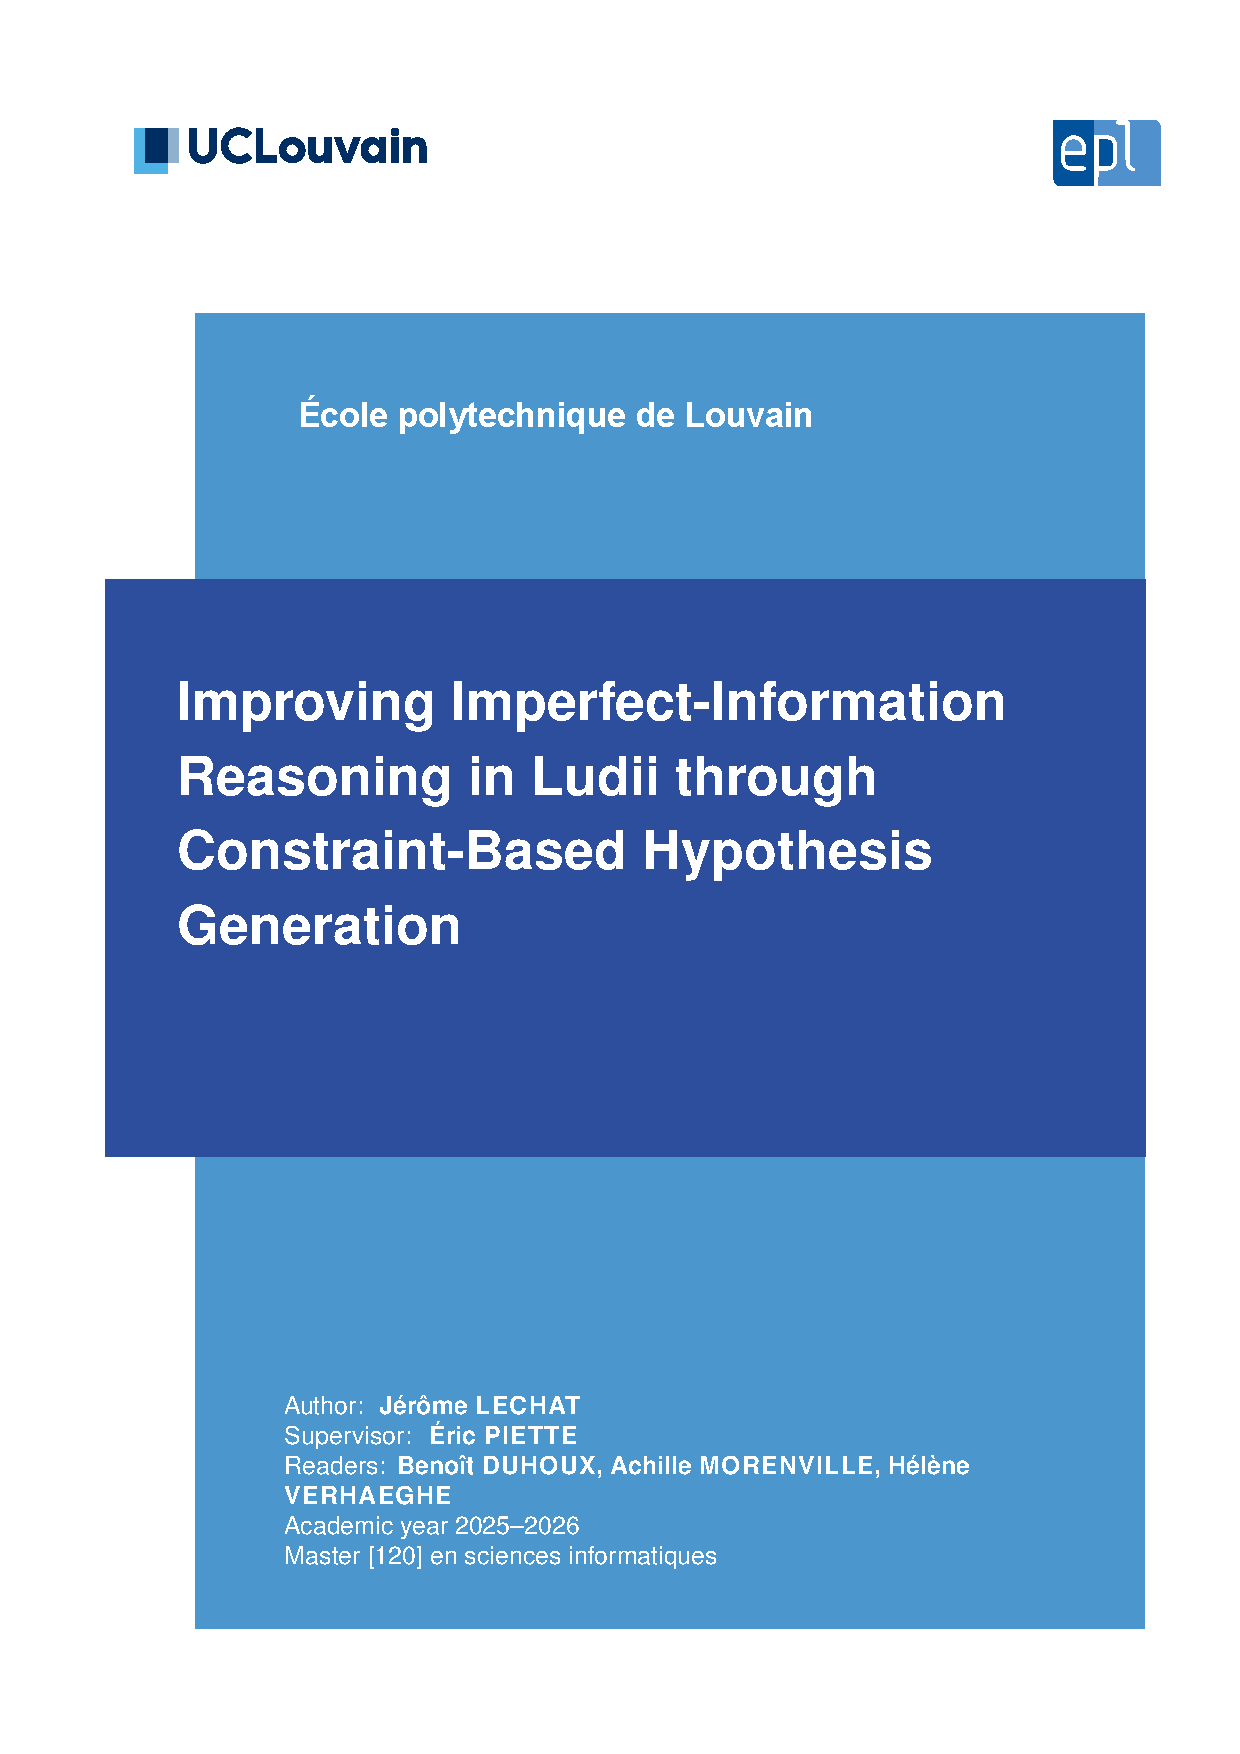
\includepdf[pages=1]{front_back/TFE26-093_EPL-master-thesis-cover.pdf}

%% The (optional) dedication can be used to thank someone or display a
%% significant quotation.
\dedication{\epigraph{Our greatest glory is not in never falling, 
    but in rising every time we fall.
  }{Nelson Mandela}}

\tableofcontents

%\chapter*{Summary}
\addcontentsline{toc}{chapter}{Summary}
\setheader{Summary}

Your summary.






\chapter*{Acknowledgments}
\addcontentsline{toc}{chapter}{Acknowledgments}
\setheader{Acknowledgments}

First and foremost, I would like to express my deepest gratitude to my supervisor, \textbf{Éric PIETTE}, for his invaluable guidance, academic support, and trust throughout this project. His expertise in General Game Playing and his insightful feedback were essential in navigating the architectural challenges of this work.

\vspace{0.5cm}

I would also like to express my sincere appreciation to my readers, \textbf{Benoît DUHOUX}, \textbf{Achille MORENVILLE}, and \textbf{Hélène VERHAEGHE}, for taking the time to review this dissertation, for their constructive criticism, and for their dedication to ensuring its academic and scientific rigor.

\vspace{0.5cm}

Computational resources have been provided by the Consortium des Équipements de Calcul Intensif (CÉCI), funded by the Fonds de la Recherche Scientifique de Belgique (F.R.S.-FNRS) under Grant No. 2.5020.11 and by the Walloon Region. Specifically, I would like to acknowledge the use of the \textbf{Dragon2} cluster hosted at the University of Mons (UMons) to collect the experimental metrics for both the Tabletop Games Framework (TAG) and the Ludii system, as well as the support and dedication of the local system administrators.

\vspace{0.5cm}

I am also deeply grateful to Google Gemini which was instrumental in the translation, grammatical correction, and rephrasing of significant portions of this dissertation.

\vspace{0.5cm}

Finally, I would like to thank \textbf{my family} from the bottom of my heart. This degree and this work belong just as much to you as they do to me. Thank you for being my anchor during the storms, for believing in me when doubt crept in, and for supporting me unconditionally when the path became difficult. Thank you for everything.

\begin{flushright}
{\makeatletter\itshape
    Jérôme \\
    LECHAT, June 2026
\makeatother}
\end{flushright}

%% Use Arabic numerals for the page numbers of the chapters.
\mainmatter

%% Turn on thumb indices.
\thumbtrue

\chapter{Introduction}
\label{introduction}

\section{Context}
Games have long served as a benchmark for \textbf{Artificial Intelligence research} because they provide well-defined rules, measurable outcomes, and controlled environments for experimentation\cite{yannakakis2025artificial}. Early successes in game AI focused primarily on \textbf{perfect-information games} such as \textbf{Chess}, \textbf{Checkers}, and \textbf{Go}, where every player has complete knowledge of the game state at all times\cite{Newborn2011Kasparov,schaeffer1996chinook,silver2016mastering}. Classical search techniques such as minimax, alpha-beta pruning, and more recently Monte Carlo Tree Search (MCTS), achieved remarkable performance in these settings, culminating in milestone systems such as \textbf{Deep Blue} against world chess champion Garry Kasparov in 1997\cite{Newborn2011Kasparov} and \textbf{AlphaGO} against the best human Go players in 2016\cite{silver2016mastering}.

However, many popular tabletop games do not follow the perfect-information assumption. Historically, \textbf{hidden information} first appeared prominently in card games, where players possess private hands unknown to their opponents. Early examples include traditional trick-taking games and later games such as Poker\cite{ParlettPokerHistory}. Over time, \textbf{hidden information mechanics} also became common in board games. Military simulation games such as Kriegsspiel introduced \textbf{fog-of-war concepts} in the nineteenth century\cite{kirschenbaum2016}, while games such as L'Attaque, Stratego, and Battleship popularized hidden identities and hidden positions in modern board game design\cite{attaque_boardgame,stratego:boardgame,battleshipgame}. Contemporary tabletop games now frequently combine board mechanics, cards, stochastic events, and multiple layers of hidden information.

This evolution fundamentally changes the nature of the AI problem. In \textbf{perfect-information games}, an agent reasons over a single fully observable game state. In \textbf{imperfect-information games}, the agent must instead reason under uncertainty, maintaining hypotheses about unknown parts of the game state and making decisions based on incomplete observations\cite{russell2020artificial, kaelbling1998planning}. This significantly increases the complexity of planning and simulation.

Two frameworks are particularly relevant for studying this problem.

The Tabletop Games Framework (TAG)\cite{gaina2020tag} is a \textbf{Java-Based research platform} specifically designed for AI benchmarking in modern board games, including games with \textbf{hidden information}. TAG gives developers explicit control over what information agents can observe during simulations, allowing agents to reason over plausible hypothetical worlds rather than the true hidden state.

Ludii\cite{piette2020ludii}, in contrast, is a large-scale General Game System hosting more than one thousand games described in a \textbf{dedicated description language}\cite{browne2020ludii_language}. Its extensive game library\cite{crist2024ludii_database} makes it an attractive platform for modern game AI research\cite{stephenson2019competition}. However, despite supporting hidden information at the game-description level, Ludii does not provide a proper mechanism for restricting hidden information that should remain hidden when copying game states during search. 

This thesis investigates this \textbf{architectural limitation} and studies how such hidden-information reasoning mechanisms inspired by TAG can be integrated into Ludii. \textbf{Battleship} was selected as the primary case study because it represents a simple but representative imperfect-information game: the opponent's ships are completely hidden, the rules are easy to formalize, and the game is computationally lightweight enough to support large-scale experiments while remaining representative of a broader class of hidden-position games.

\section{Architectural Challenges}
General Game Playing (GGP)\cite{Genesereth2005GeneralGP} systems are AI frameworks designed to support many different games through a common simulation and agent infrastructure, without requiring game-specific AI implementations. Reasoning under hidden information is not only a game-design challenge but also an architectural challenge for such systems. Most classical GGP frameworks were originally designed around \textbf{perfect-information assumptions}, where every simulation can safely operate on an exact copy of the current game state\cite{Love+al:2006}. In \textbf{imperfect-information games}, however, this assumption no longer holds: an agent should only reason from the information that is observable to the corresponding player.

This creates a fundamental difficulty for simulation-based AI methods such as Monte Carlo Tree Search (MCTS)\cite{browne2012survey}, Rolling Horizon Evolution\cite{perez2018rolling}, or One-Step Look-Ahead\cite{gaina2020tag}. These algorithms repeatedly copy and simulate game states in order to evaluate future actions. In \textbf{perfect-information games}, unrestricted state copies are correct and desirable. In \textbf{imperfect-information games}, the copied state must instead preserve the uncertainty faced by the player. Hidden information should therefore be masked, randomized, or replaced with plausible hypotheses during simulations\cite{cowling2012information}.

TAG was explicitly designed with this requirement in mind. Its architecture allows developers to control how game states are copied for each player, making it possible to generate player-specific observations and coherent determinizations during search. As a result, agents reason over hypothetical worlds that are consistent with their observations rather than over the true hidden state.

Ludii follows a different architectural philosophy. While hidden information can be expressed correctly at the game-description level through the .lud language, the simulation infrastructure itself relies on unrestricted copies of the game context\cite{soemers2021playouts}. Consequently, agents performing simulations may access information that should remain hidden, such as the exact positions or identities of opponent pieces. This behavior is not intentional cheating by the agents, but rather a consequence of an architecture originally designed primarily for perfect-information reasoning.

This limitation has important methodological consequences for AI research. If agents can unintentionally exploit privileged information during simulations, experimental results can no longer be interpreted as measurements of genuine reasoning under uncertainty. Comparisons between agents become biased, and the evaluation of imperfect-information algorithms becomes unreliable.

Addressing this issue is particularly challenging in a General Game Playing setting. Unlike specialized game engines, GGP systems must support many different games without relying on game-specific implementations. Any solution must therefore remain generic, compatible with existing agents, and applicable across a large and heterogeneous game library.

The central objective of this thesis is to address this architectural limitation in Ludii by introducing a determinization layer inspired by TAG’s hidden-information handling mechanisms. The proposed approach aims to preserve compatibility with existing Ludii agents while ensuring that simulations operate on coherent hypothetical game states rather than on privileged information.

\section{Research Objectives}
This thesis investigates how hidden-information reasoning can be integrated into a GGP framework originally designed around perfect-information assumptions. More specifically, the work studies how simulation-based AI agents can operate on coherent hypothetical game states rather than on privileged information during search.

To address this problem, the thesis pursues three main objectives.

\textbf{The first objective} is to establish a controlled imperfect-information benchmark in the Tabletop Games Framework (TAG) using Battleship as a case study. This benchmark serves as a reference environment for studying determinization strategies under hidden information. Three levels of determinization are developed and evaluated: BASIC, which relies on naive random determinization; SMART, which generates hypotheses consistent with previously observed hits and misses through a constraint-based approach; and SMART+HEATMAP, which extends SMART with a probabilistic heatmap used to bias action selection toward statistically likely ship positions. These implementations provide a controlled baseline for imperfect-information reasoning in TAG.

\textbf{The second objective} is to formally characterize the hidden-information simulation problem in Ludii. This involves analyzing the architectural differences between TAG and Ludii, studying how game-state copies are generated during simulations, and demonstrating that native simulation-based Ludii agents may unintentionally access privileged hidden information during search. The impact of this behavior is then evaluated experimentally through controlled tournaments in Battleship.

\textbf{The third and central objective} is to design and implement a generic determinization layer for Ludii inspired by TAG’s hidden-information handling mechanisms. The proposed solution intercepts simulation copies, replaces hidden information with coherent hypotheses generated from past observations, and integrates transparently with existing simulation-based Ludii agents without requiring modifications to their internal decision logic\cite{piette2021ludii_logic}. The approach is evaluated experimentally and compared against the TAG reference benchmark in order to assess both its effectiveness and its limitations.
 
\section{Thesis Structure}
The remainder of this thesis is organized as follows:

\textbf{Chapter 2} introduces the theoretical and technical background required for the study. It presents the main concepts related to imperfect-information games, determinization techniques, simulation-based AI methods, and General Game Playing frameworks. The architectures and hidden-information mechanisms of both TAG and Ludii are also discussed.

\textbf{Chapter 3} develops the reference benchmark used throughout the thesis. Battleship is implemented in TAG, and several determinization strategies are designed and evaluated in order to study the impact of hidden-information handling on agent performance.

\textbf{Chapter 4} analyzes the hidden-information simulation problem in Ludii. The chapter studies how state copies are generated during simulations and demonstrates how unrestricted copies may expose privileged information to agents during search.

\textbf{Chapter 5} presents the proposed determinization layer for Ludii. The architecture of the solution is described in detail, including hidden-information detection, game-state reconstruction, hypothesis generation, and integration with existing simulation-based agents.

\textbf{Chapter 6} evaluates the proposed approach experimentally through a series of controlled tournaments in Ludii and compares the results against the TAG reference benchmark.

Finally, \textbf{Chapter 7} summarizes the main contributions of the thesis, discusses the limitations of the proposed approach, and outlines several directions for future work.
\chapter{Background}
\label{Background}

\begin{abstract}
This chapter introduces the theoretical and technical background required for the remainder of the thesis. It first presents the main concepts related to General Game Playing and imperfect-information games, including determinization and simulation-based search methods. It then introduces the two frameworks studied in this work, TAG and Ludii, with a particular focus on their approaches to hidden-information handling and game-state simulation.
\end{abstract}

%%% GGP %%%
\section{General Game Playing (GGP)}
GGP\cite{Genesereth2005GeneralGP} is a field of Artificial Intelligence that studies the design of agents capable of playing many different games through a common decision-making architecture. Unlike specialized game-playing systems, which are developed and optimized for a single game, GGP agents must operate without game-specific tuning. The rules of the game are provided as input, and the agent is expected to interpret them and generate strategies autonomously.

The field emerged prominently through the \hyperlink{http://ggp.stanford.edu/}{Stanford General Game Playing project}\footnote{Available at \url{http://ggp.stanford.edu/}} and the AAAI General Game Playing Competition, where games were described using the Game Description Language (GDL)\cite{Love+al:2006}. This approach introduced the idea of reusable game-independent AI agents capable of reasoning over arbitrary rule systems. Over the years, the competition contributed to the development of increasingly sophisticated GGP agents, including systems such as CADIAPLAYER\cite{finnsson2009cadiaplayer} and Woodstock, the latest champion of the General Game Playing competition\cite{koriche2017symmetry,koriche2017woodstock}.

Since then, GGP research has expanded toward increasingly diverse game domains, including video games through the General Video Game AI (GVGAI) framework\cite{Genesereth2005GeneralGP}, stochastic games, multi-player environment, and modern board games.

Modern tabletop games introduce several challenges that are uncommon in traditional perfect-information games such as Chess or Go. These games often include hidden information, stochastic events, large branching factors, and complex interactions between heterogeneous game components. As a result, agents can no longer rely solely on deterministic search over a fully observable game state. They must instead reason under uncertainty and evaluate actions using incomplete observations and hypothetical world states.

The General Game Playing community has long recognized this limitation. Extensions such as GDL-II were introduced to support imperfect-information and stochastic games within the GGP paradigm\cite{Genesereth2005GeneralGP}. These extensions allow game descriptions to represent hidden information and partial observability at the rule level. However, correctly handling imperfect information requires more than simply encoding hidden data in the game description. The simulation infrastructure itself must preserve uncertainty during search and prevent agents from accessing privileged information when generating hypothetical future states.

This distinction is central to the architectural differences between TAG and Ludii studied in this thesis. While both frameworks support hidden information at the game-definition level, they differ significantly in how uncertainty is preserved during simulation and state copying.

%%% (IM)PERFECT INFORMATIONS %%%
\section{Information}
\subsection{Perfect and Imperfect}
In game theory, a game is said to have perfect information if every player has complete knowledge of the game state at all times\cite{russell2020artificial}. Classical examples include Chess, Go, and Tic-Tac-Toe, where all pieces and previous actions are fully observable to every player throughout the game. In such environments, decision-making algorithms can reason directly over a single fully observable game state.
\begin{figure}[H]
    \centering % Centre l'ensemble des deux images sur la largeur de la page
    
    % Première image (gauche)
    \begin{minipage}[H]{0.45\textwidth}
        \centering
        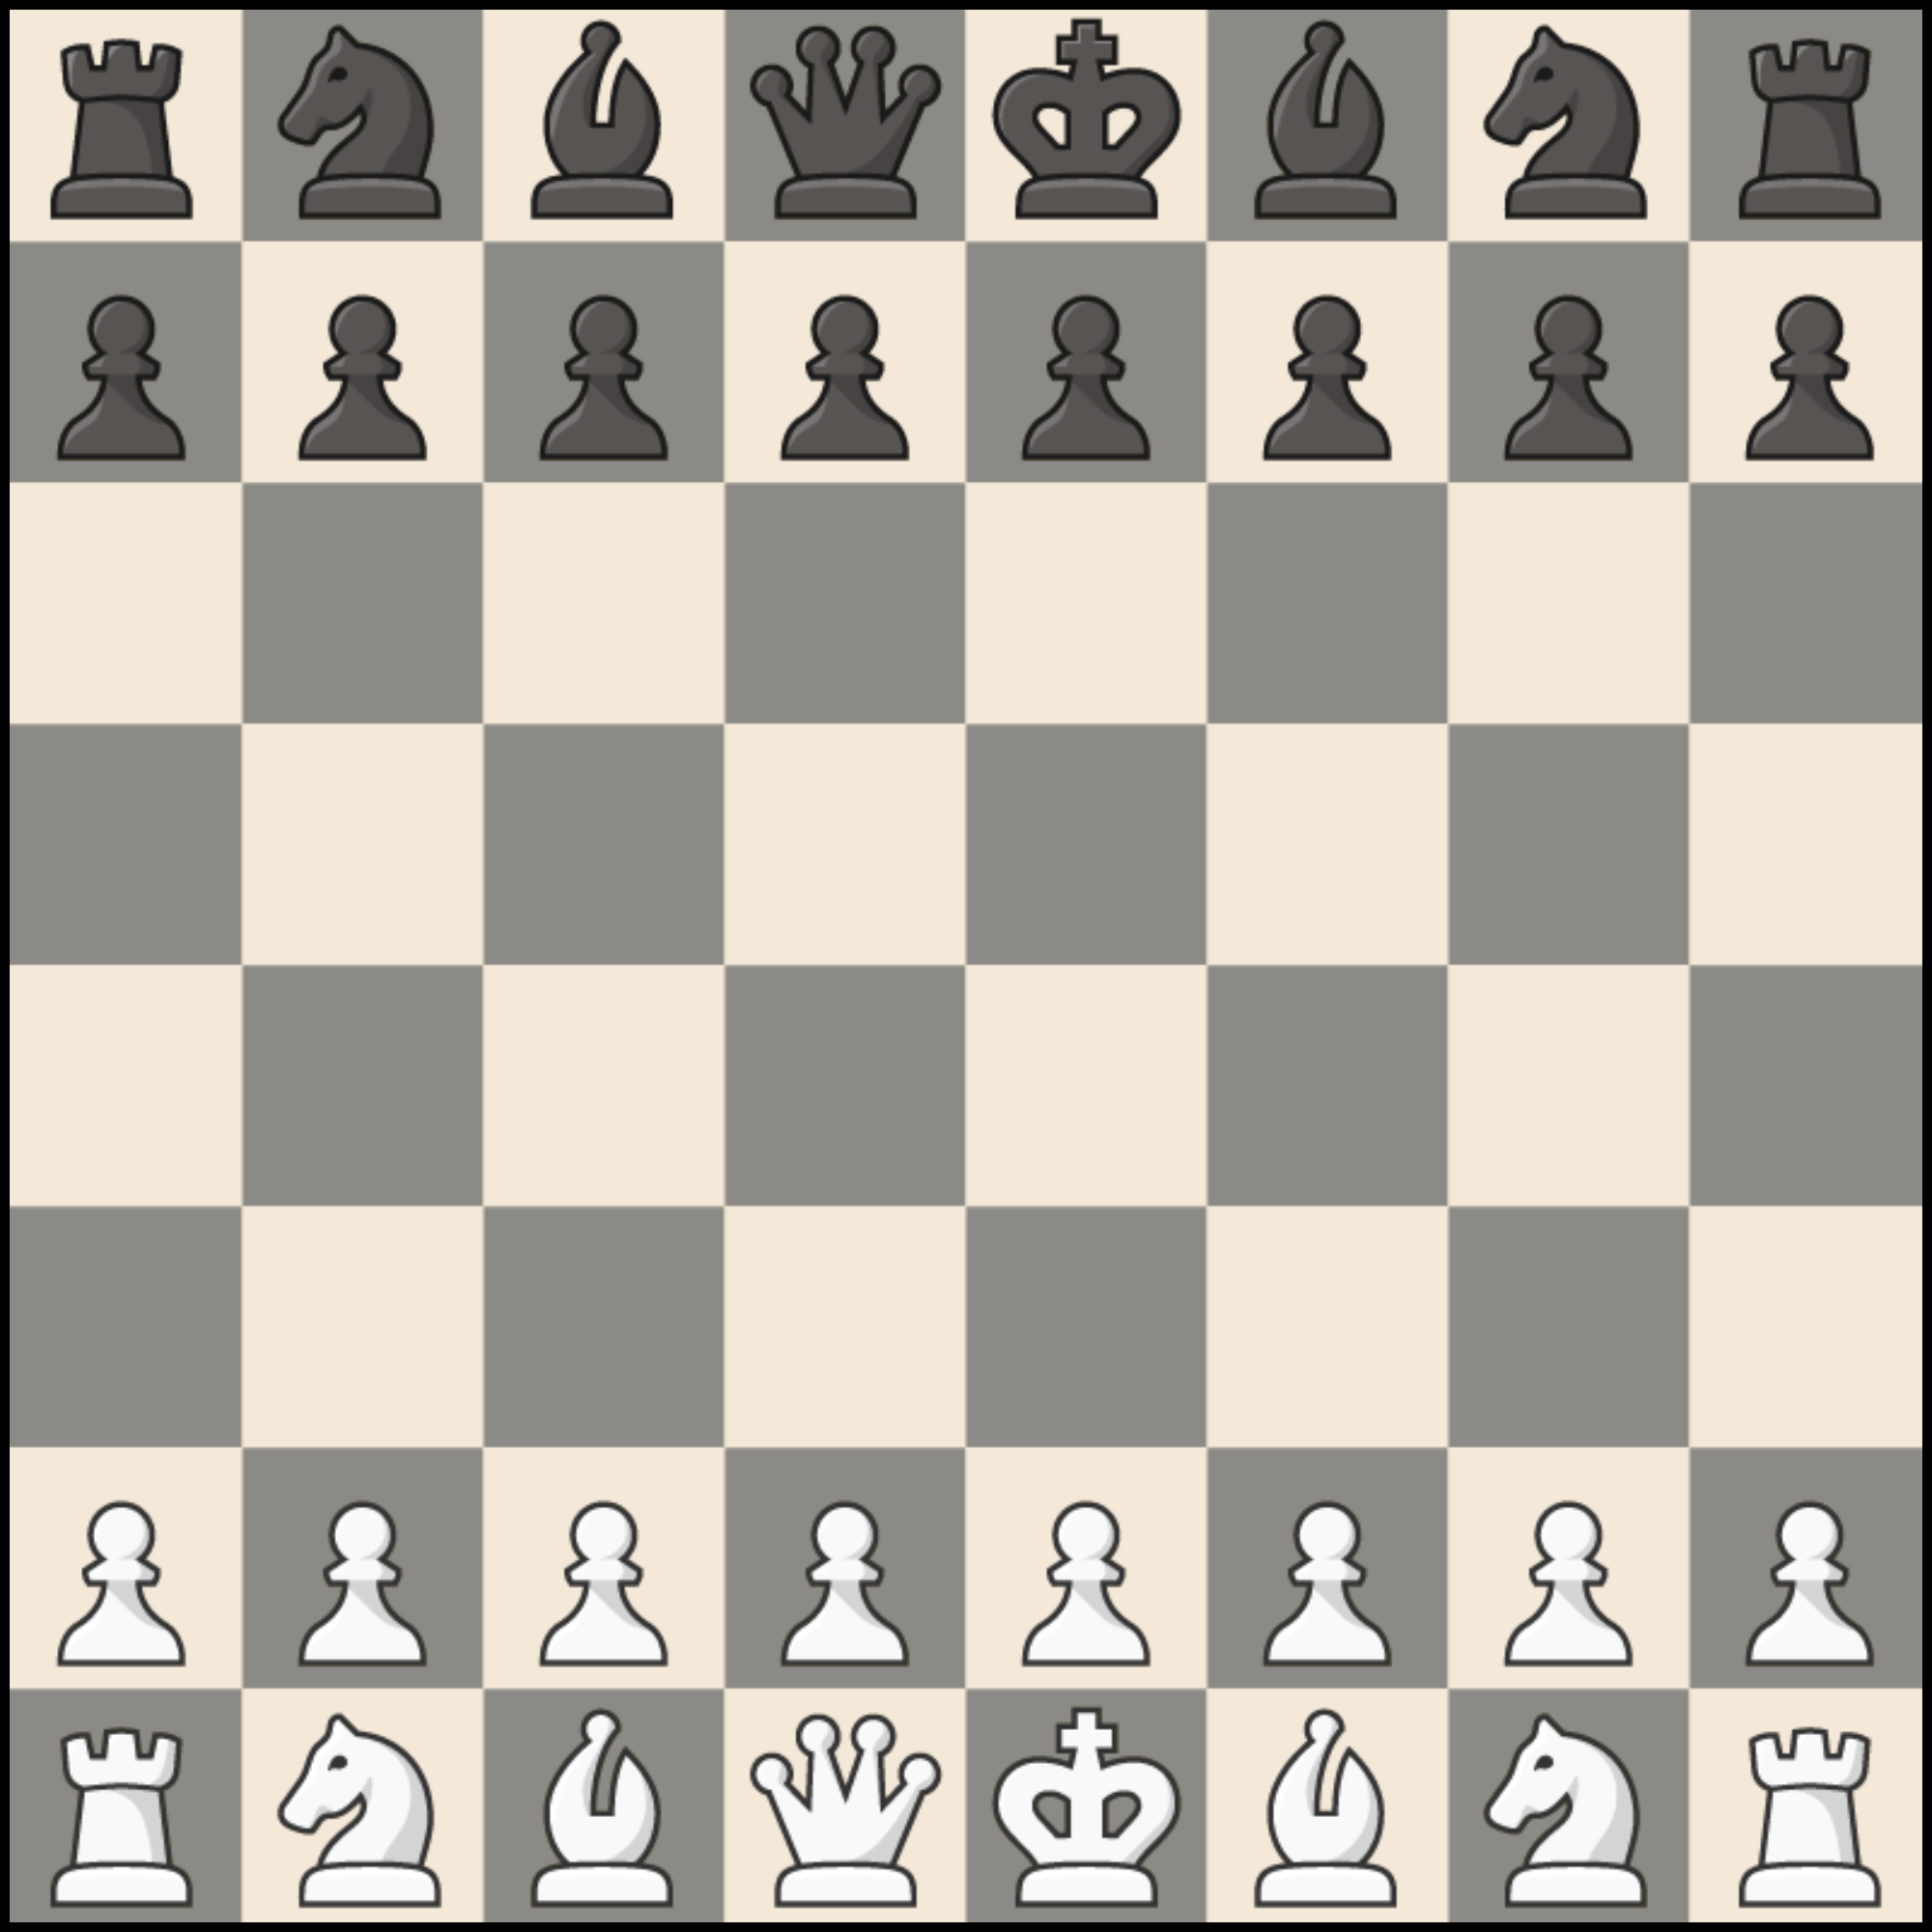
\includegraphics[width=0.75\textwidth]{figs/chess.png}
    \end{minipage}
    \hfill % Crée l'espace entre les deux images
    % Deuxième image (droite)
    \begin{minipage}[H]{0.45\textwidth}
        \centering
        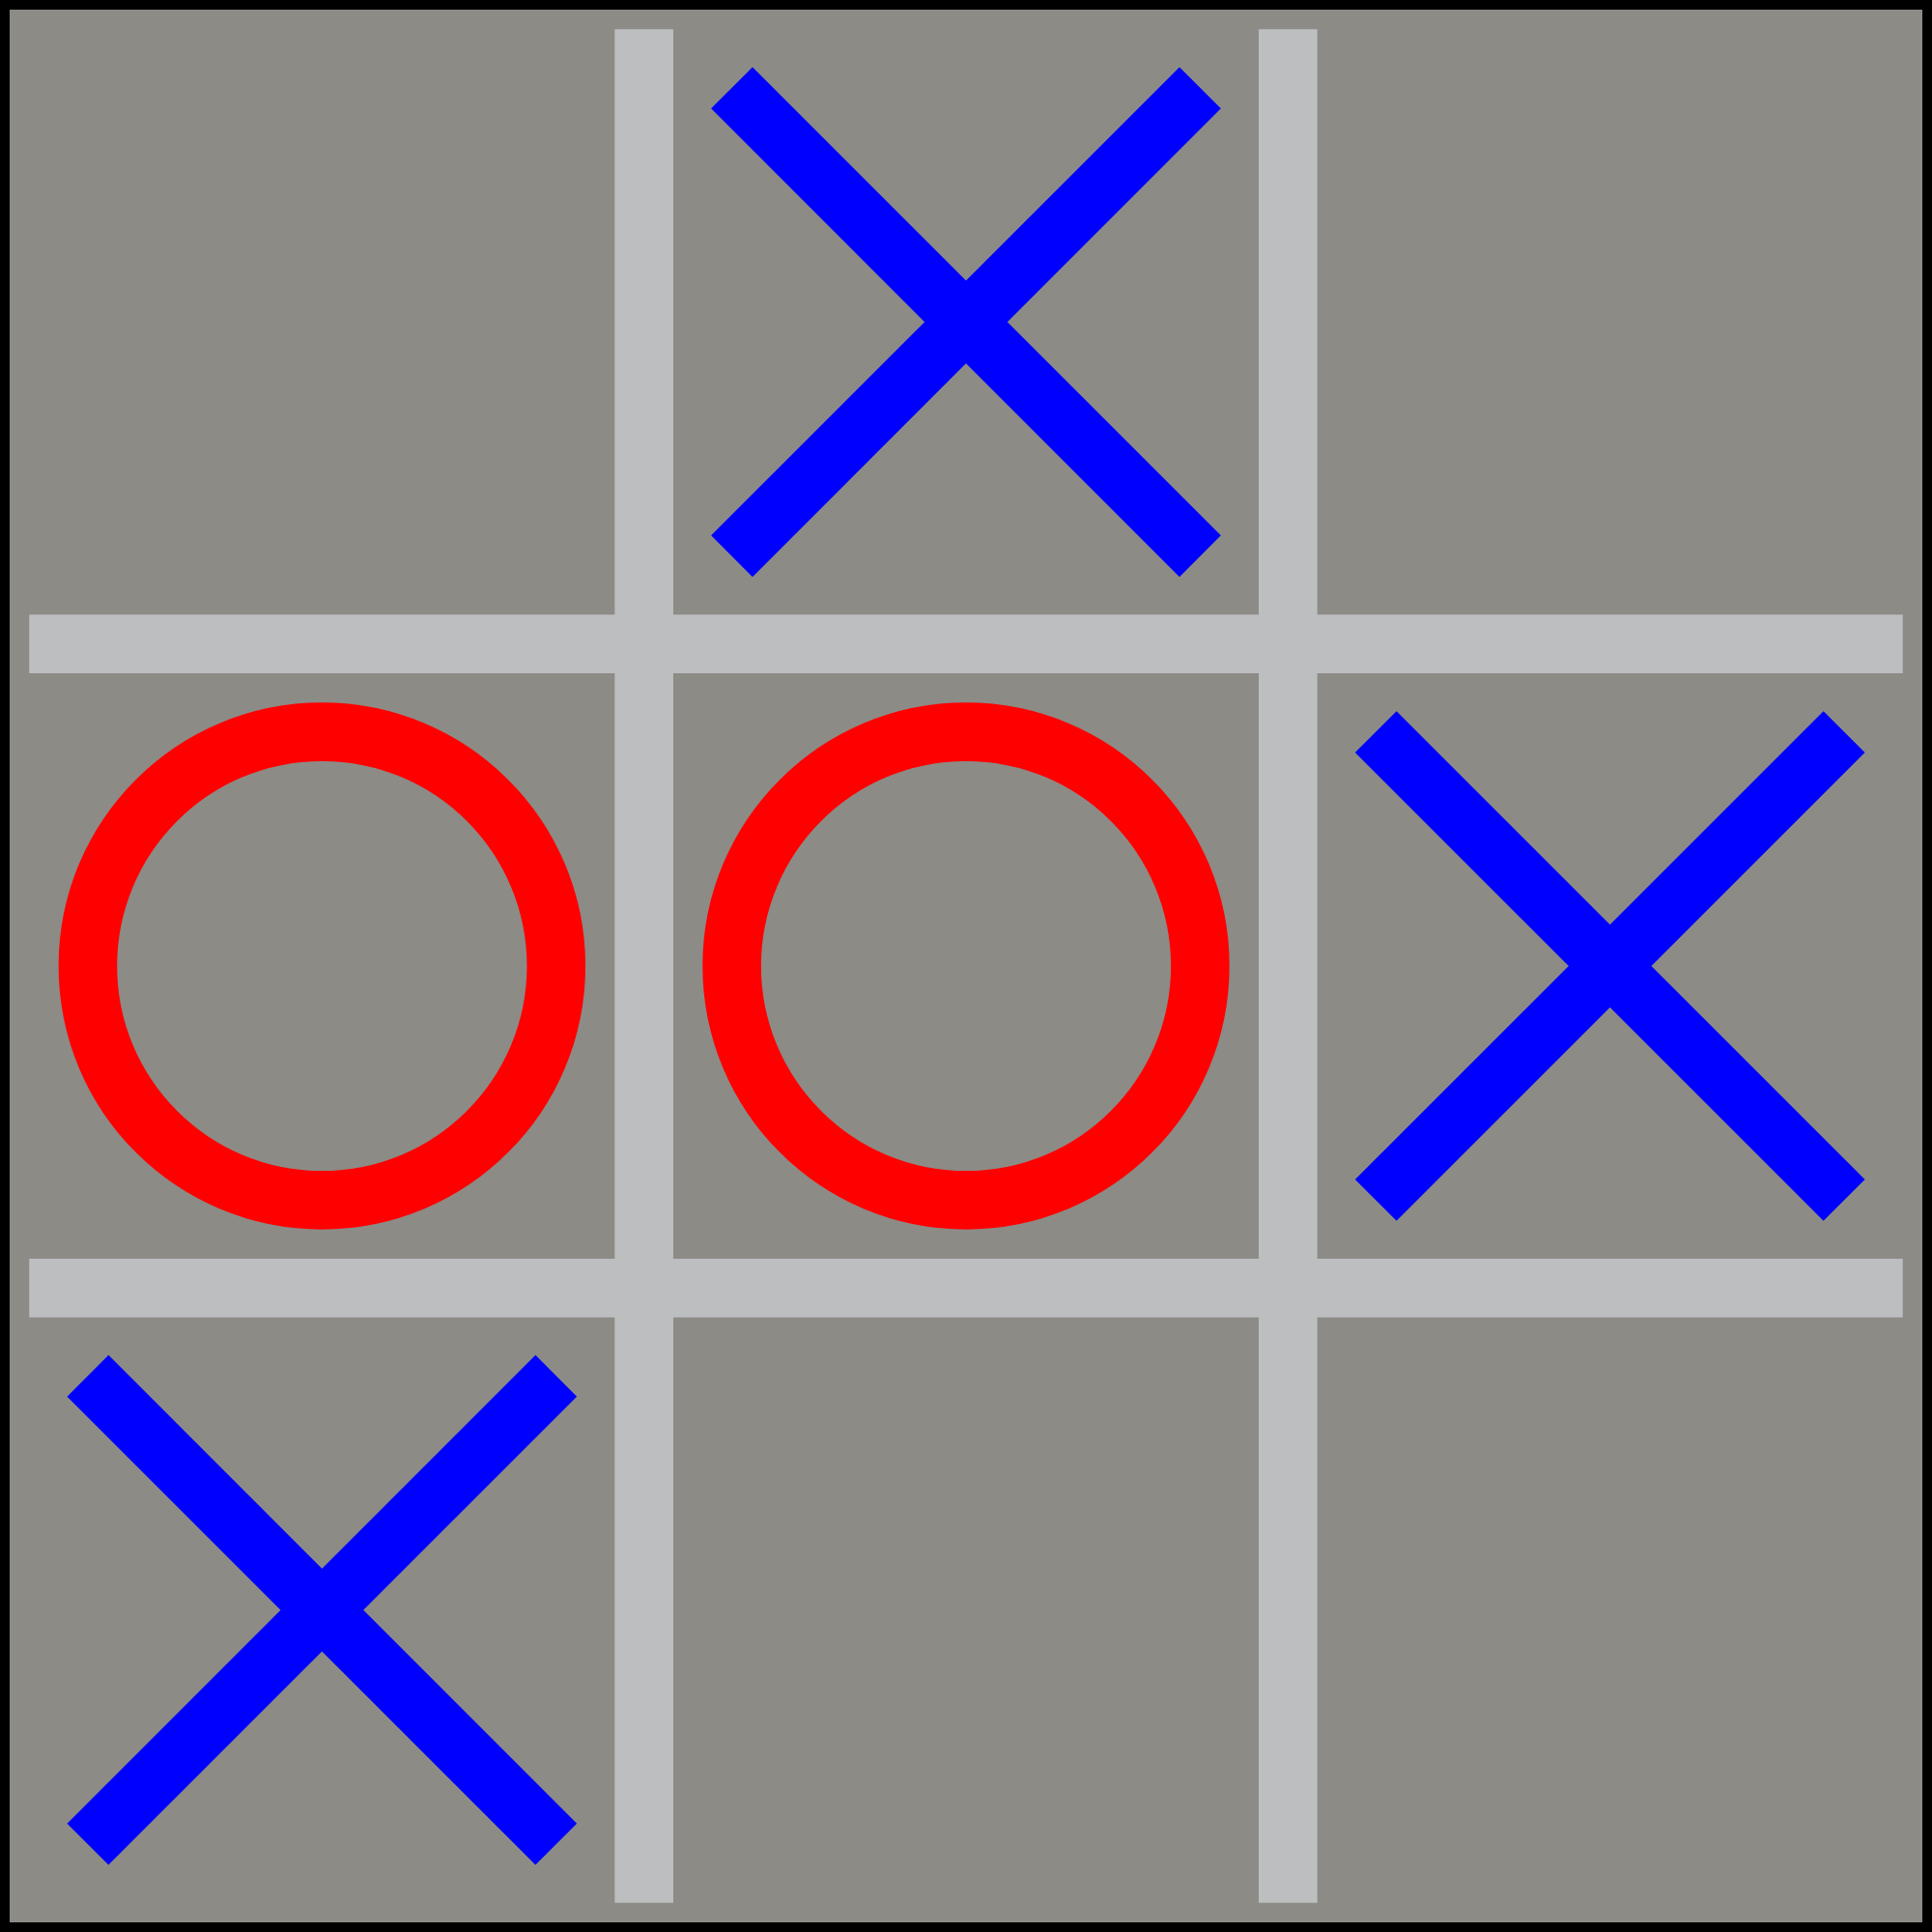
\includegraphics[width=0.75\textwidth]{figs/tictactoe.png}
    \end{minipage}

    \vspace{0.15cm} % Petit espace vertical avant la légende
    \captionsetup{justification=centering}
    \caption{In games like chess and TicTacToe, both players have a total visibility of the state of the game.}
    \label{fig:example_of_perfect_information_games}
\end{figure}

In contrast, a game has imperfect information when some aspects of the game state are hidden from at least one player\cite{russell2020artificial}. This hidden information may concern private cards, concealed pieces, secret objectives, or unknown positions on the board. Examples include Poker, Stratego, Battleship, and Mahjong. In these games, players must reason under uncertainty and make decisions based on incomplete observations. This distinction has major implications for Artificial Intelligence. In perfect-information games, agents can evaluate future actions by simulating deterministic transitions from a known state. In imperfect-information games, however, the agent must additionally reason about unknown elements of the environment and maintain hypotheses regarding the hidden parts of the game state.

\subsection{Different Types of Hidden information}
Hidden information can appear in many different forms depending on the game mechanics and the nature of the uncertainty involved\cite{kaelbling1998planning}. Previous work has explored several categories of imperfect-information structures, including hidden actions, hidden objectives, simultaneous decisions, stochastic uncertainty, and partially observable state transitions\cite{bowling2015heads}. The Valet game suite, for example, was specifically designed to study diverse forms of hidden information and uncertainty in tabletop games\cite{goadrich2026valet}. 

This thesis focuses on two forms of hidden state information that are particularly relevant for simulation-based reasoning in board games.

The first category concerns hidden identities. In this case, the location of a game object is visible, but its type or value is unknown. In Stratego, for example, players can observe the positions of opponent pieces without knowing their ranks. Similarly, in many card games, players know how many cards their opponents hold without knowing the exact cards themselves.

\vspace{0.5cm}
\noindent
\begin{minipage}[c]{0.45\textwidth}
    \centering
    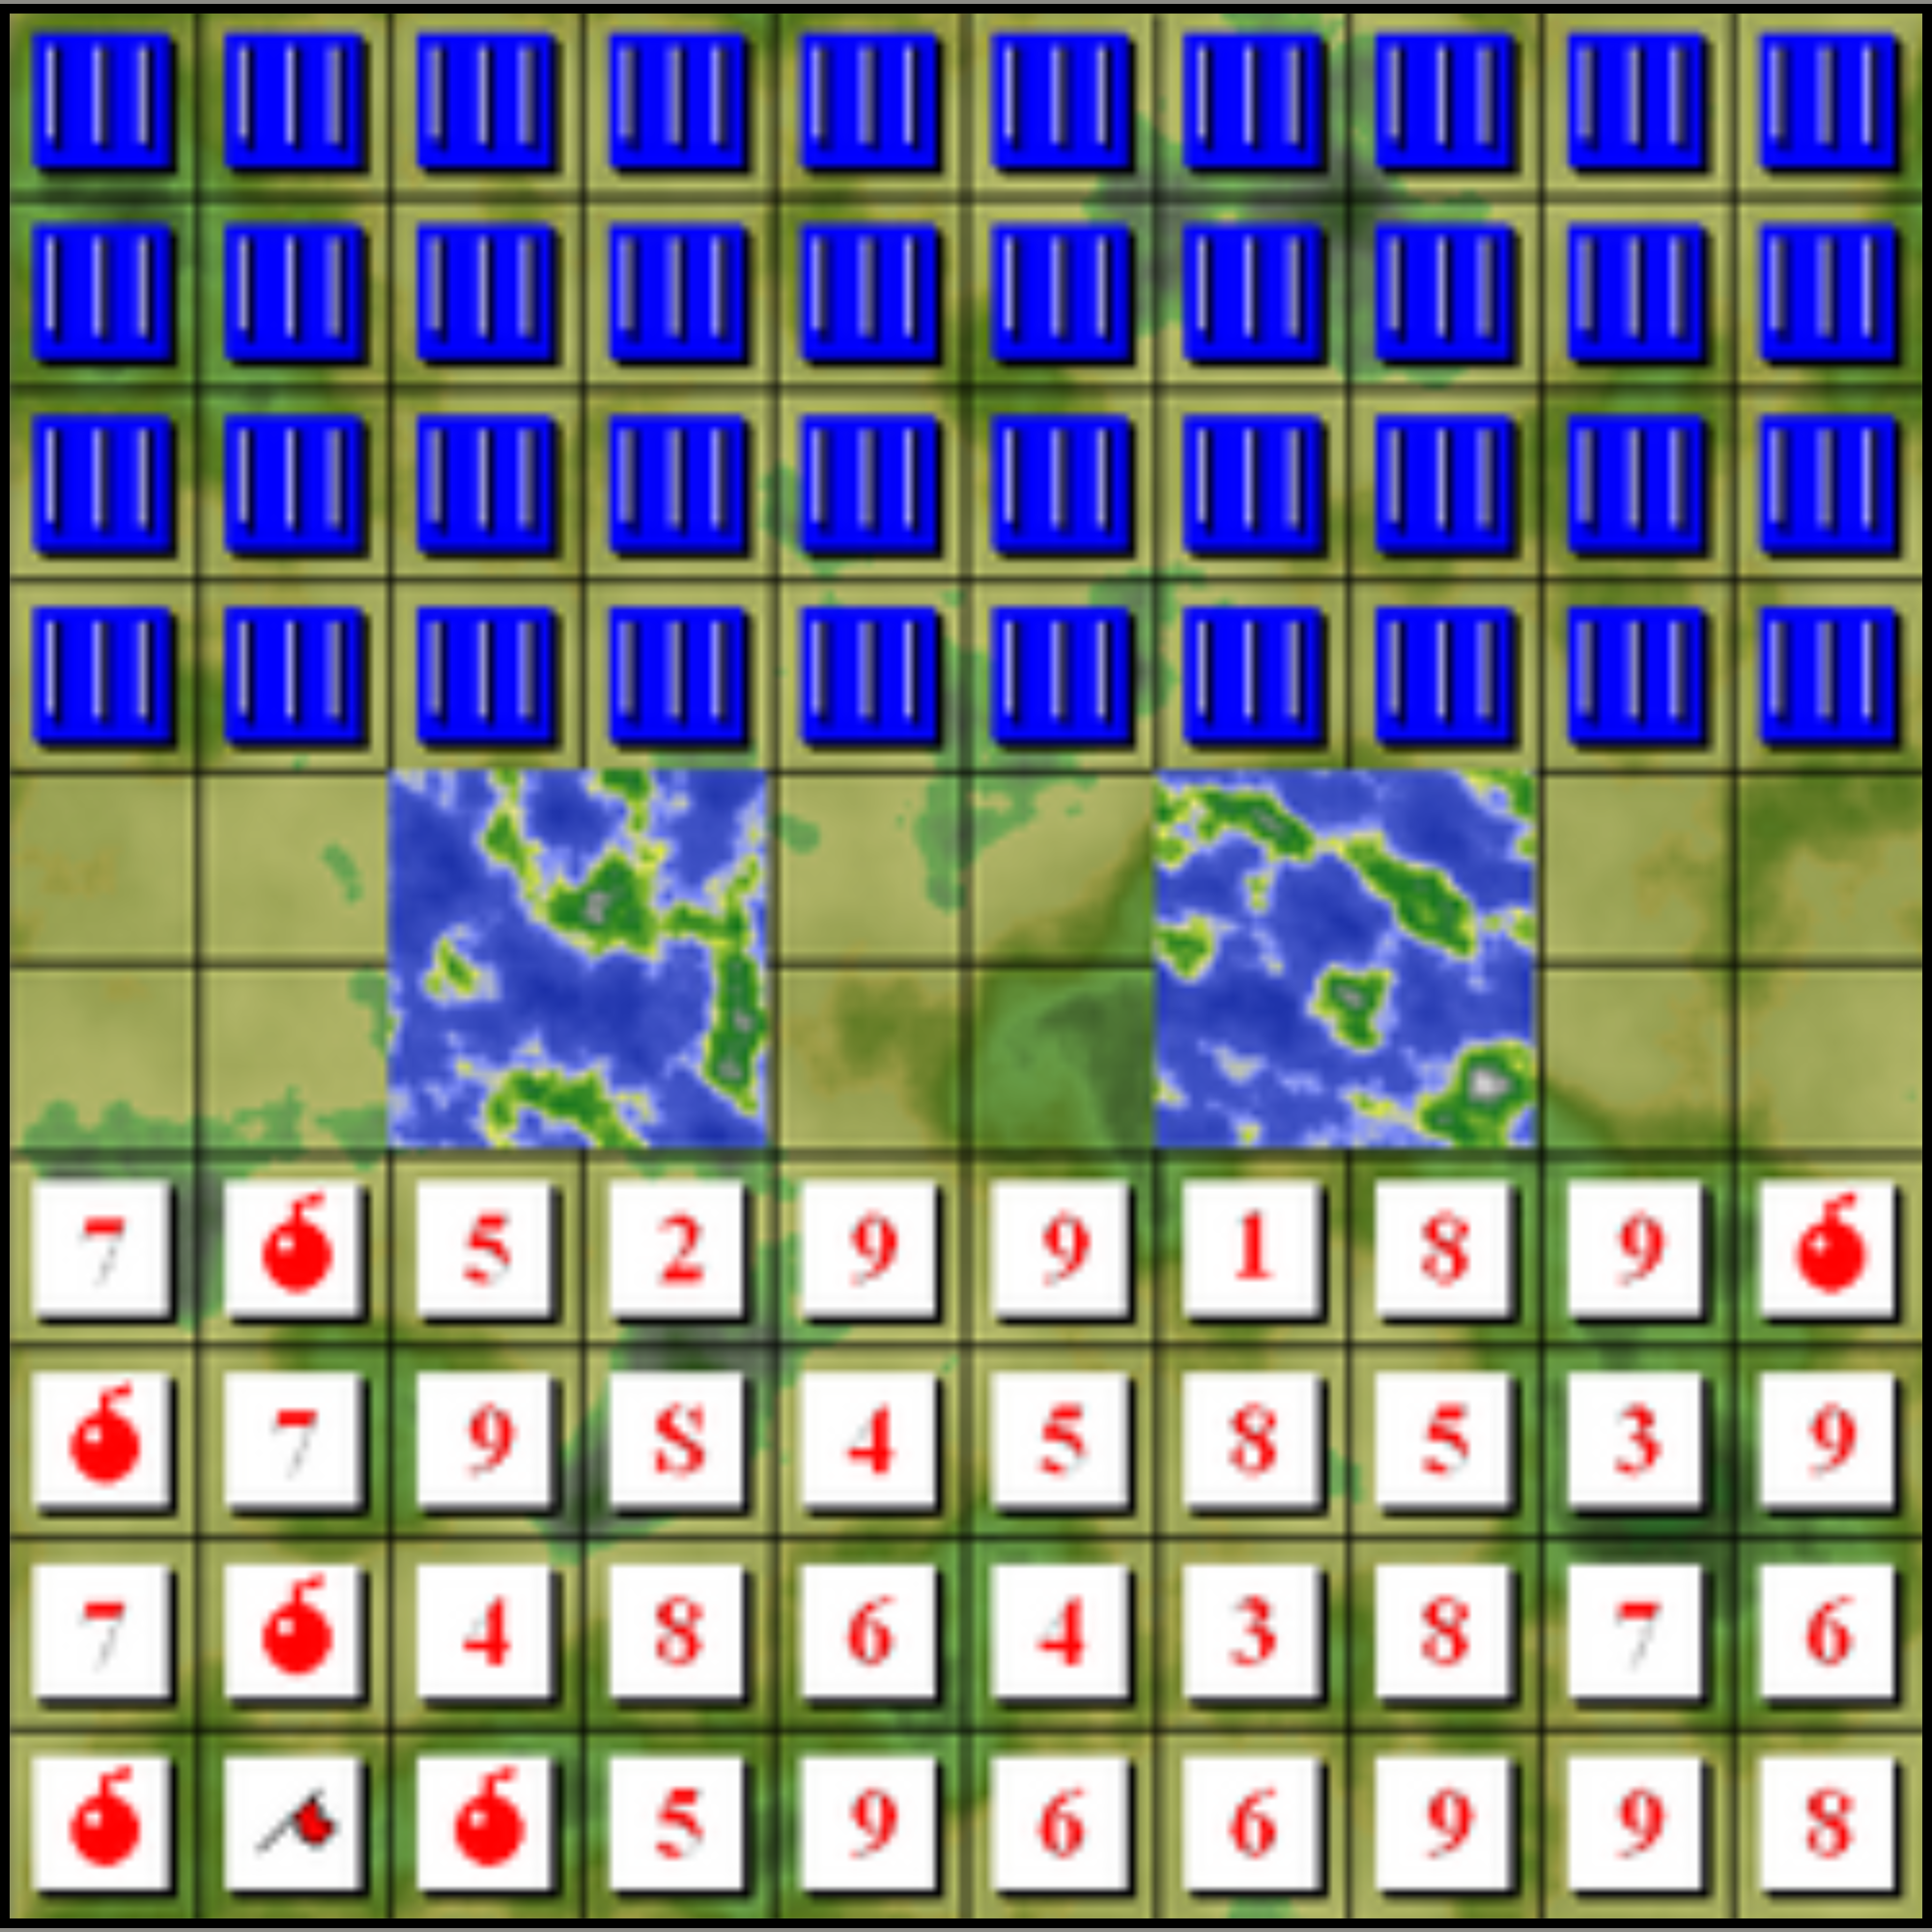
\includegraphics[width=0.80\textwidth]{figs/stratego.png}
    \captionsetup{hypcap=false}
    \captionof{figure}{We know the locations, but not the values.}
    \label{fig:stratego}
\end{minipage}
\hfill
\begin{minipage}[c]{0.50\textwidth}
    \textbf{Unknown identity of pieces}: The agent knows where a game object is, but not what it is. In Stratego, for instance, you can see that there is an opponent piece on a certain square, but you do not know its rank. In card games, you know your opponent has cards in hand, but not which ones.
\end{minipage}

The second category concerns hidden positions. In this case, the existence or location of objects is itself unknown. Battleship is a representative example: the opponent’s ships are completely hidden, and the player has no direct information regarding their positions on the grid.

\noindent
\begin{minipage}[H]{0.50\textwidth}
    \textbf{Unknown position of pieces}: The agent does not know where certain objects are at all. In Battleship, the opponent's ships are completely hidden: you do not even know in which region of the board they are. \textbf{This is the category that this thesis focuses on.}
\end{minipage}
\hfill
\begin{minipage}[H]{0.45\textwidth}
    \centering
    
\includegraphics[width=0.80\textwidth]{figs/battleship.png}
    \captionsetup{hypcap=false}
    \captionof{figure}{We don't know the locations of the enemy's ships and their values.}
    \label{fig:battleship}
\end{minipage}

This distinction has important consequences for AI reasoning. Hidden-identity games constrain uncertainty to known locations, whereas hidden-position games require the agent to reason over a significantly larger space of possible configurations. In hidden-position settings, the agent must first infer plausible locations before meaningful strategic planning can occur. Battleship belongs primarily to this second category and therefore provides a useful benchmark for studying determinization techniques under spatial uncertainty.

\subsection{Information Sets}
In extensive-form game theory, uncertainty is commonly represented through the notion of an Information Set\cite{Osborne1994}. In imperfect-information games, a player generally cannot determine the exact current game state because some elements of the environment remain hidden. Instead, multiple possible states may be consistent with the observations available to the player.

An Information Set therefore represents the collection of game states that are indistinguishable from the perspective of a given player at a particular moment in the game. Each state within the set is compatible with the player’s observations, the sequence of previously observed actions, and the known rules of the game. Two examples help illustrate this concept.

\textbf{In Poker}, if a card has been publicly revealed during gameplay, players may know part of an opponent’s hand while remaining uncertain about the remaining hidden cards. The corresponding Information Set contains all valid card distributions consistent with the revealed information.
\begin{figure}[H]
    \centering % Centre l'ensemble des deux images sur la largeur de la page

    % image
    \begin{minipage}[H]{\textwidth}
        \centering
        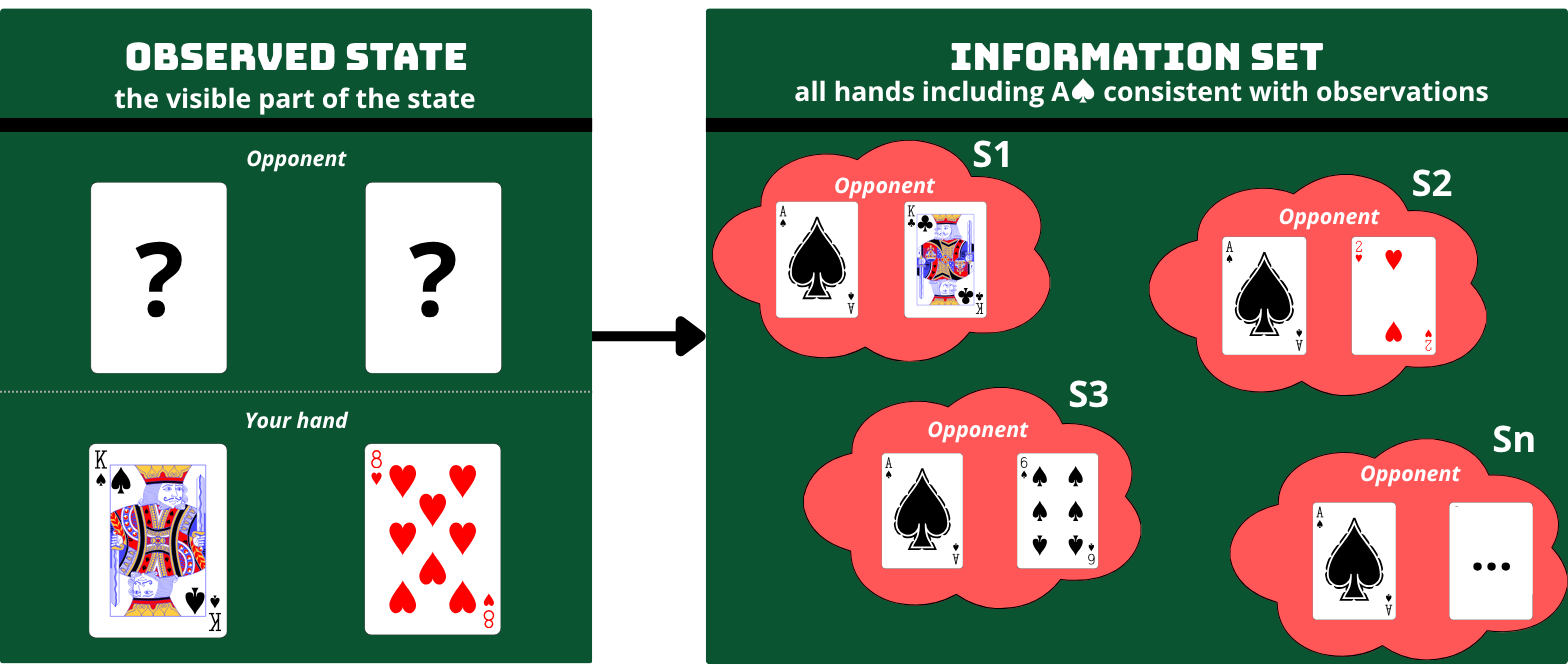
\includegraphics[width=1\textwidth]{figs/background/poker.png}
    \end{minipage}
    \captionsetup{justification=centering}
    \caption{All world configurations containing the Ace of Spades}
    \label{fig:poker}
\end{figure}

\textbf{In Battleship}, after observing a sequence of hits and misses, the Information Set contains all ship configurations compatible with these observations. Every additional shot progressively eliminates impossible configurations and reduces the number of plausible hidden states.

\newpage

Information Sets provide a formal framework for reasoning under uncertainty in imperfect-information games. However, explicitly representing all possible states quickly becomes computationally intractable in many practical settings. In Battleship, for example, the number of valid ship configurations at the beginning of the game is extremely large, making exhaustive enumeration impractical for simulation-based AI methods.

As a result, imperfect-information game AI systems often rely on approximate representations of uncertainty rather than explicit enumeration of complete Information Sets. This naturally leads to approaches based on belief states and determinization, which are introduced in the next section.

\subsection{Belief State and Determinization}
A common approach for reasoning under uncertainty consists in representing the player’s knowledge through a belief state: a probability distribution over all game states consistent with the observations available to the agent\cite{kaelbling1998planning}. As new observations become available during gameplay, this distribution can be updated to reflect changes in the player’s uncertainty regarding the hidden parts of the environment.

In theory, an optimal imperfect-information agent would reason directly over this belief distribution when selecting actions. In practice, however, maintaining and updating exact belief states is often computationally infeasible because the number of possible hidden configurations grows extremely rapidly in many games.

Consequently, practical imperfect-information AI systems frequently rely on approximate methods. One widely used approximation is determinization\cite{long2010understanding,cowling2012information}. Instead of reasoning over the full belief distribution, the agent samples or generates a plausible fully instantiated game state consistent with the currently available observations. The search algorithm then operates on this hypothetical state as if it were the true game state.

The quality of the determinization has a direct impact on the quality of the resulting simulations. If the generated hypothetical state is inconsistent with previous observations or highly implausible, the simulations performed by the agent may provide misleading evaluations and poor action recommendations.

Several simulation-based search algorithms rely on determinization techniques to operate in imperfect-information environments. These algorithms are introduced in the next section.

%%% AGENTS %%%
\section{Search Algorithms}
This section introduces the main simulation-based agents used throughout this thesis. These algorithms are representative baseline methods commonly used in GGP and modern board game AI research. While some were originally designed for perfect-information environments, several can be extended to imperfect-information settings through the use of determinization techniques.

\subsection{Random Agent}
The Random agent is the simplest possible baseline. At each turn, it selects one legal action uniformly at random without performing any evaluation or look-ahead.

Despite its simplicity, Random agents remain important in AI benchmarking because they provide a lower performance bound for comparison. Any search-based agent should consistently outperform a purely random policy in order to demonstrate meaningful strategic reasoning.

\subsection{One-Step Look-Ahead (OSLA)}
One-Step Look-Ahead (OSLA)\cite{gaina2020tag} is a greedy search method that evaluates the immediate consequence of each legal action before selecting a move. For every available action, the agent simulates a single forward step and evaluates the resulting state using a heuristic function, such as score estimation or game-specific features. The action producing the highest evaluation is then selected.

OSLA performs only shallow search and therefore cannot anticipate long-term consequences beyond the next state. Nevertheless, because it directly exploits information from simulated future states, it often provides significantly stronger performance than purely random play while remaining computationally inexpensive.

\subsection{Rolling Horizon Evolution (RMHC)}
Rolling Horizon Evolution (RHEA)\cite{perez2018rolling} is an online planning approach based on evolutionary optimization. Instead of constructing an explicit search tree, the agent maintains sequences of future actions representing candidate plans. These plans are iteratively modified through mutation operators and evaluated by simulating their execution in the game environment.

At each decision step, the best-performing action sequence is selected, the first action is executed, and the planning horizon is shifted forward for the next turn. Because the optimization process continuously replans during gameplay, the method is commonly referred to as a rolling horizon approach.

A simple and widely used variant is the Rolling Horizon Mutation Hill Climber (RMHC) \cite{perez2018rolling}, where candidate plans are optimized through repeated random mutations and greedy replacement. RHEA-based methods are particularly effective in environments with large action spaces where exhaustive tree search becomes difficult.

\subsection{Monte Carlo Tree Search (MCTS)}
Information Set Monte Carlo Tree Search (IS-MCTS)\cite{cowling2012information} extends MCTS to imperfect-information environments through the use of determinization. Instead of constructing the search tree from a single fully observable state, IS-MCTS repeatedly samples hypothetical game states consistent with the observations available to the player.

During search, simulations are therefore performed across multiple determinizations rather than a single known world state. This allows the agent to reason under uncertainty while still relying on standard forward simulations.

The effectiveness of IS-MCTS strongly depends on the quality of the determinization process. If sampled hypothetical states are inconsistent with previous observations or highly implausible, the resulting simulations may provide poor guidance for action selection. Consequently, the generation of coherent determinizations plays a central role in imperfect-information search performance.

\subsection{Move-Average Sampling Technique (MAST)}
The Move-Average Sampling Technique (MAST)\cite{chaslot2008progressive} is an enhancement commonly used with MCTS to improve rollout quality. Instead of selecting actions uniformly at random during simulations, MAST maintains statistics regarding the average reward historically associated with actions encountered across previous simulations.

These statistics are then used to bias rollout policies toward actions that performed well in the past, typically through epsilon-greedy or softmax selection strategies. By replacing purely random simulations with statistically informed rollouts, MAST can significantly improve search efficiency without requiring domain-specific heuristics.

Because MAST remains game-independent while improving simulation quality, it is frequently used as a general enhancement for GGP agents and modern board game AI systems.

%%% TBG VS MBG %%%
\section{Traditional Board Games \& Modern Board Games}
Traditional board games, such as Chess, Go, or Checkers, are typically characterized by \textbf{perfect information} and \textbf{simple, deterministic rules.} All players have full access to the complete game state at all times, and there is no hidden information. As a result, these games are well suited for classical AI techniques, including minimax search, alpha-beta pruning, and Monte Carlo Tree Search (MCTS)\cite{russell2020artificial}. Many early General Game Playing (GGP) systems were designed with this type of game in mind\cite{Genesereth2005GeneralGP}. On the other side, \textbf{modern board games} introduce a bigger variety of mechanics that significantly increase their complexity. These games often include \textbf{hidden information}, such as private hands of cards, secret objectives, or concealed board elements. They may also feature stochastic elements, large and dynamic action spaces, and complex interactions between game components. Examples include card-driven games, bluffing games, and games with fog-of-war or hidden spatial layouts. This difference has important consequences for AI research. While traditional board games allow agents to reason over a fully known and static game state, modern board games require agents to operate under \textbf{uncertainty.} The agent must make decisions based on incomplete observations and assumptions about unknown parts of the game state. As a result, AI techniques designed for perfect-information games often perform poorly or become invalid when applied directly to modern board games. Therefore, supporting modern board games requires frameworks that can explicitly represent hidden information and provide mechanisms for reasoning under uncertainty. This distinction motivates the need for platforms such as TAG and highlights the limitations of existing GGP systems that were originally designed for traditional games.

%%% TAG %%%
\section{The Tabletop Games Framework (TAG)}
\subsection{Overview of TAG}
TAG\cite{gaina2020tag} is a Java-based research framework designed for benchmarking AI agents on modern tabletop games. The framework was developed to address limitations of earlier GGP systems, which primarily focused on classical perfect-information games. TAG instead targets modern tabletop environments that frequently involve stochasticity, multi-player interactions, and hidden information.

TAG currently includes implementations of numerous modern board and card games, together with a standardized experimental infrastructure for AI evaluation\cite{gaina2023design}. The framework provides reusable implementations of several simulation-based agents, tournament management tools, and detailed logging systems capable of recording gameplay statistics such as branching factors, action-space sizes, hidden-information levels, and win rates. This infrastructure facilitates controlled and reproducible experimentation across multiple games and agent configurations.

Beyond academic research, the framework has also contributed to practical applications in tabletop game development. In particular, TAG served as the foundation for \hyperlink{https://www.tabletoprnd.co.uk/}{Tabletop R\&D}\footnote{Available at \url{https://www.tabletoprnd.co.uk/}}, a spin-out initiative focused on AI-assisted board game analysis, balancing, and automated playtesting. This illustrates the growing practical relevance of modern tabletop game AI beyond purely academic benchmarking.

\subsection{Code-First Design}
TAG follows a code-first design philosophy in which games are implemented directly in Java rather than described through a dedicated game description language. This approach provides developers with substantial flexibility regarding game logic, state representation, and simulation behavior.

Because games are implemented programmatically, developers can directly control hidden-information handling, optimization strategies, and custom mechanics that may be difficult to express declaratively. This flexibility is particularly important for imperfect-information research, where the way game states are copied and observed during simulations has a direct impact on agent behavior.

The main limitation of this approach is scalability. Implementing a new game requires writing a dedicated Java implementation, which demands significantly more development effort than declarative game-description systems such as Ludii.

\subsection{Architecture}
\textbf{TAG} uses an \textbf{MVC (Model-View-Controller)} architecture, which is a standard software design pattern that separates data (\textbf{M}odel), visual presentation (\textbf{V}iew), and decision logic (\textbf{C}ontroller). 
In the context of game AI, this makes it easy to implement new games and plug in new AI agents without modifying the core framework.



The \textbf{M}odel consists of three abstract classes that must be implemented for each game:
\begin{itemize}
    \item The \textbf{AbstractGameState} stores everything about the current game state: the board, the pieces, the scores, the current player, and any hidden information.

    \item The \textbf{AbstractForwardModel} handles the game logic. It generates the list of legal actions via \textsc{\_computeAvailableActions()}, applies them to the game state, and checks end conditions in \textsc{\_afterAction()}.

    \item The \textbf{AbstractParameters} stores the configurable parameters of the game, such as grid size or ship sizes in Battleship for example.
\end{itemize}
Implementing a new game in TAG requires writing these three classes. The framework handles everything else (turn management, logging, tournament running, and result analysis).

\medskip

The \textbf{V}iew consists of GUI components: \textbf{AbstractGUIManager} and \textbf{\textit{game-specific board views}} that render the game state visually. The GUI is optional and not required for AI experiments. 

\medskip

The \textbf{C}ontroller is \textbf{Game.java}, which orchestrates the game loop. At each turn, it calls the forward model to compute available actions, passes them to the current agent, and applies the chosen action to the game state.

\begin{figure}[H]
    \centering % Centre l'ensemble des deux images sur la largeur de la page
    
    \begin{minipage}[H]{1\textwidth}
        \centering
        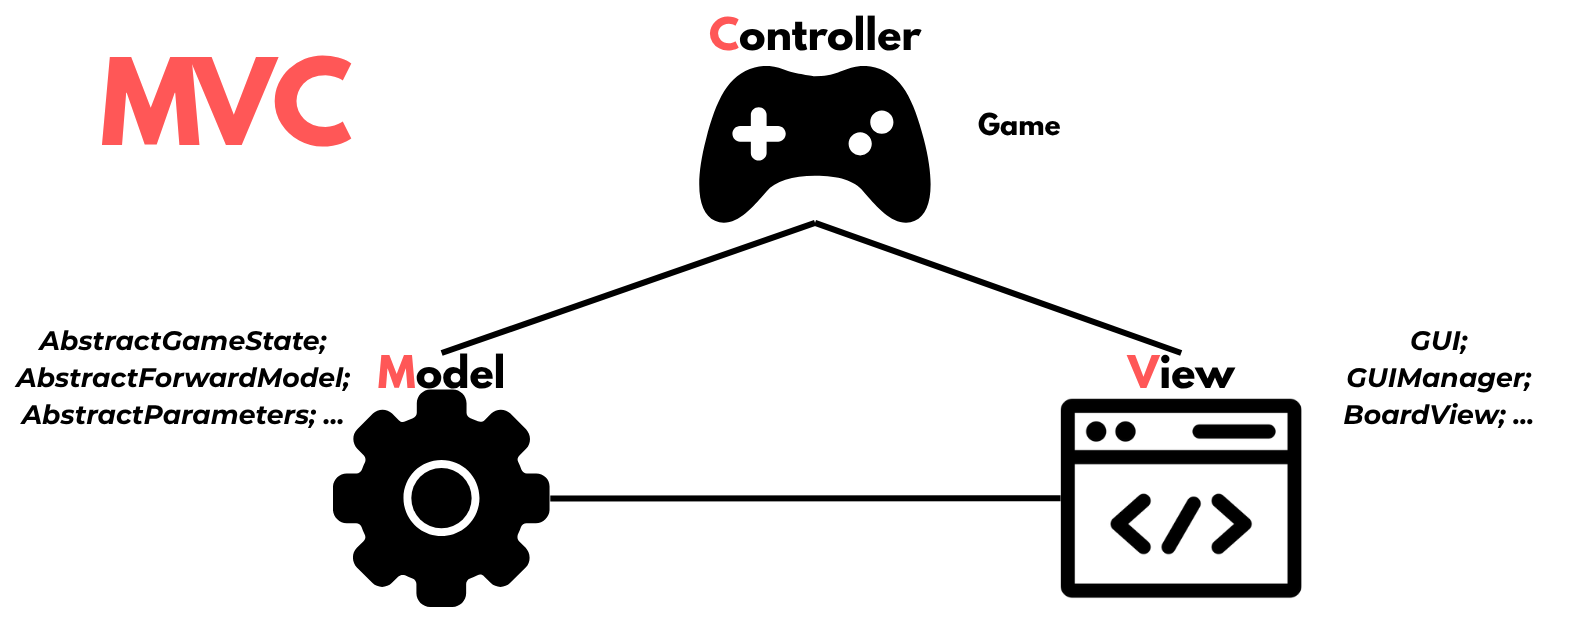
\includegraphics[width=1\textwidth]{figs/background/MVC.png}
    \end{minipage}

    \vspace{0.15cm} % Petit espace vertical avant la légende
    \captionsetup{justification=centering}
    \caption{TAG's Model-View-Controller (MVC) Architecture}
    \label{fig:TAG_MVC_Architecture}
\end{figure}

\subsection{Agent Interface and State Copying}
AI agents in TAG extend the AbstractPlayer class and implement a decision function that selects an action from the current game state and the list of legal actions.

\begingroup
\captionsetup[lstlisting]{justification=centering}
\begin{lstlisting}[language=Java, caption={Abstract method for selecting an action from available legal moves}, label=lst:basic-deter, basicstyle=\ttfamily\small, columns=fullflexible, keepspaces=true]
public abstract AbstractAction _getAction(AbstractGameState gameState, List<AbstractAction> possibleActions);
\end{lstlisting}
\endgroup

A key architectural feature of TAG is its support for player-specific state copies. During simulations, agents do not necessarily receive the true underlying game state. Instead, the framework allows the game implementation to generate customized observations through player-dependent copy mechanisms.

This design is particularly important for imperfect-information games. Hidden information can be masked, randomized, or replaced with coherent hypothetical states before simulations are performed. As a result, agents reason over observations and determinizations that are consistent with the information available to the corresponding player rather than over privileged hidden information.

This explicit control over simulation copies makes TAG especially suitable for research on imperfect-information reasoning and determinization techniques.

\subsection{Current Limitations}
Despite its flexibility for AI experimentation, TAG also presents several limitations. Its game library remains relatively small compared to large-scale General Game Playing systems such as Ludii, and every new game requires a dedicated manual implementation in Java.

Furthermore, because TAG does not rely on a declarative game description language, rapidly prototyping or modifying game variants can require substantial development effort. These limitations motivate the interest in complementary frameworks capable of supporting much larger game libraries while still enabling robust imperfect-information reasoning.


%%% LUDII %%%
\section{The Ludii General Game Playing System}
\subsection{Overview of Ludii}
Ludii\cite{piette2020ludii} is a General Game Playing framework designed to support a very large and diverse collection of games through a unified game description system\cite{piette2020ludii}. Unlike code-first frameworks such as TAG, Ludii follows a data-first approach in which games are described declaratively using a dedicated language known as the Ludii Game Description Language (.lud)\cite{browne2020ludii_language}. The framework originated from the Digital Ludeme Project\cite{browne2022dlpworkshop}, an initiative focused on the historical reconstruction, analysis, and study of traditional games through computational methods. Ludii was developed as the central software platform supporting this effort by providing a unified representation system capable of modeling games from many different historical periods and cultural traditions\cite{crist2024ludii_database}. Today, the framework continues to be actively maintained and is used extensively within the GameTable COST Action research network\cite{piette2024gametable_kickoff} for experimentation, game analysis, and AI benchmarking across large collections of tabletop games\cite{browne2023ludii}.

Ludii was originally designed around the concept of ludemes, which represent conceptual units of game rules and mechanics\cite{piette2021concepts}. By combining ludemes hierarchically, the framework can represent a wide range of board, card, dice, and multiplayer games within a common formal system. Ludii currently includes \hyperlink{https://ludii.games/library.php}{more than one thousand playable games from diverse cultural and historical contexts}\footnote{Available at \url{https://ludii.games/library.php}}.

One of Ludii’s major strengths is its scalability for GGP research. Because games are described declaratively rather than implemented manually in code, new games and variants can often be created rapidly with relatively limited development effort. This makes Ludii particularly attractive for large-scale experimentation, comparative game studies\cite{rautureau2026gametable_opening}, procedural game generation\cite{todd2024gavel}, and automated AI benchmarking across diverse game libraries\cite{piette2019ludii_rbg}.

In addition to classical perfect-information games such as Chess and Go, Ludii also supports stochastic and imperfect-information games through dedicated language constructs. Hidden information can be specified declaratively within the game description, allowing the framework to represent mechanisms such as hidden hands, concealed identities, and partially observable game elements.

However, representing hidden information at the game-description level does not necessarily guarantee correct imperfect-information reasoning during simulation. As discussed in the following sections, the way game states are copied and exposed to agents during search plays a critical role in determining whether uncertainty is properly preserved during AI simulations.

\subsection{Data-First Design}
Unlike code-first frameworks such as TAG, Ludii represents games through declarative `.lud` descriptions composed of ludemes. Rather than implementing game logic manually in procedural code, developers define games through hierarchical combinations of reusable rule components.

This design introduces an additional abstraction layer between the game definition and the underlying simulation engine. AI agents therefore interact with generic game representations generated from the declarative description rather than with manually customized game implementations.
For instance, the following extract from \textbf{Battleships.lud} describes how hidden information is set up at the start of the game:
\begin{center}
    \begin{verbatim}
        (set Hidden (sites P1 "Defence") to:P2)
        (set Hidden (sites P2 "Defence") to:P1)
    \end{verbatim}
\end{center}
This tells Ludii that player 1's defence zone is hidden from player 2, and vice versa. The hidden information is encoded directly in the game description, no Java code is needed.

Such abstraction provides important advantages for GGP research. Because games share a common internal representation structure, the same AI agents, analysis tools, and experimental pipelines can be reused across many different games with limited adaptation.

However, this abstraction also creates challenges for imperfect-information reasoning. In code-first systems, developers can explicitly customize how hidden information is exposed to players during simulations. In declarative systems such as Ludii, hidden-information handling must instead emerge from generic engine-level mechanisms capable of operating across many different game types.

As a consequence, correctly preserving uncertainty during simulation becomes an architectural problem extending beyond the game description itself. This distinction is central to the hidden-information limitations studied in this thesis.

\subsection{Architecture}
Ludii transforms declarative .lud descriptions into executable game representations through an internal compilation process. Once compiled, games are executed through a collection of generic runtime objects responsible for storing game states, applying rules, and managing simulations.

\begin{figure}[H]
    \centering % Centre l'ensemble des deux images sur la largeur de la page
    
    \begin{minipage}[H]{1\textwidth}
        \centering
        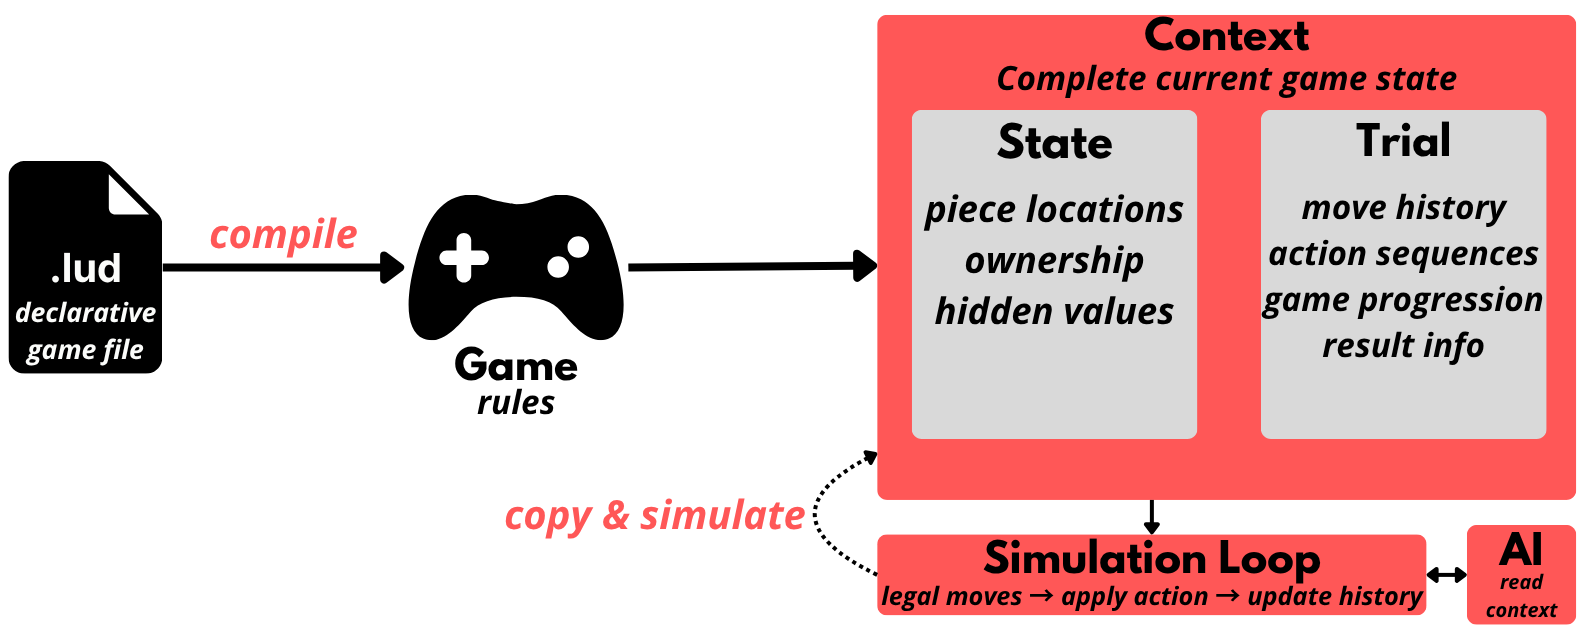
\includegraphics[width=1\textwidth]{figs/background/ludiiARCH.png}
    \end{minipage}

    \vspace{0.15cm} % Petit espace vertical avant la légende
    \captionsetup{justification=centering}
    \caption{Ludii's Architecture}
    \label{fig:ludii_architecture}
\end{figure}

One of the central runtime objects is the Context, which represents the complete current state of an ongoing game. The Context contains all information required to continue gameplay, including board configurations, player data, hidden information, scores, random generators, and references to previous actions. The Context itself contains two important substructures:
\begin{itemize}
    \item \textbf{State}, which stores the current mutable state of the game, such as piece locations, ownership, hidden values, and phase information.

    \item \textbf{Trial}, which records the history of actions performed during the game, including move sequences and game progression information.
\end{itemize}
Together, these structures provide the information required by AI agents during gameplay and search. Game progression is managed through generic rule execution mechanisms. At each decision step, Ludii generates the legal moves available from the current Context, applies selected actions to produce successor states, and updates the corresponding game history. Because this process is implemented generically at the engine level, the same simulation infrastructure can operate across many different game types without requiring game-specific AI implementations. Simulation-based agents typically evaluate future actions by repeatedly copying the current Context and performing forward simulations on the copied state. This mechanism is efficient for perfect-information games because the copied context fully represents the exact current game state.

However, in imperfect-information environments, the copied Context may also contain hidden information that should not be accessible to the acting player during search. Consequently, the semantics of state copying become particularly important for preserving uncertainty correctly during simulations. This issue is examined in the following sections.

\subsection{Hidden Information Representation}
Ludii supports imperfect-information games through dedicated language constructs integrated directly into the .lud description system. These constructs allow game designers to specify which parts of the game state are visible or hidden to different players during gameplay.

Hidden information in Ludii is represented primarily through visibility rules associated with game elements and state variables. Depending on the game, these rules may hide the identity of pieces, their positions, the ownership of components, private hands, or other game-specific information from selected players.

The framework distinguishes several forms of hidden information, including hidden values (What), hidden ownership (Who), hidden state variables (State), hidden counts (Count), and hidden positions (Where)\cite{piette2021ludii_logic}. This representation allows a broad range of imperfect-information mechanics to be modeled declaratively within a unified system.

For example, in Stratego, the positions of pieces remain visible while their identities are hidden, corresponding primarily to hidden What information. In Battleship, by contrast, ship positions themselves are hidden, corresponding mainly to hidden Where information. More complex games may combine several hidden-information dimensions simultaneously.

These visibility rules are correctly enforced during normal gameplay and player interaction. Human players and graphical interfaces only receive information that should be observable according to the game rules. Consequently, Ludii is fully capable of representing imperfect-information games at the game-definition and gameplay levels.

However, representing hidden information during gameplay is distinct from preserving uncertainty during AI simulations. While visibility rules determine what information is observable to players, simulation-based agents often operate on internal game states generated through generic copying mechanisms. Whether hidden information remains protected during search therefore depends not only on the visibility system itself, but also on how simulation contexts are generated and exposed to agents during forward planning.

\subsection{Simulation and State Copying}
Simulation-based agents in Ludii evaluate future actions by repeatedly generating copies of the current Context and performing forward simulations on these copied states. This mechanism is used extensively by search algorithms.

The Context object contains the complete internal game state, including information that may be hidden from individual players in imperfect-information games. Consequently, when a simulation-based agent copies the current context during search, the copied state may still contain privileged hidden information.

This behavior is not problematic in perfect-information games, where all players already have full access to the game state. In imperfect-information environments, however, simulations should ideally operate on hypothetical states that remain consistent with the information actually observable by the acting player.

The challenge therefore lies in generating simulation states that preserve uncertainty during search rather than exposing the full underlying game state to the agent. From an architectural perspective, this requires mechanisms capable of constructing player-compatible determinizations from incomplete observations before forward simulations are performed.

Addressing this problem constitutes the primary technical objective of this thesis. The following chapters investigate how determinization mechanisms inspired by TAG can be integrated into Ludii in order to preserve hidden-information uncertainty during simulation-based search.

%\section{Related Work}
%\begin{center}
    %\doublebox{
        %\begin{minipage}{\textwidth}
            %\centering
                %\textbf{\colorbox{yellow}{TODO: Recent update, still have to write it properly}}
        %\end{minipage}
    %}
%\end{center}
\chapter{Determinization in TAG Using Battleship}
\label{BattleshipInTAG}

\begin{abstract}
This chapter presents the TAG-based benchmark developed to study determinization quality in imperfect-information environments. Battleship is used as the reference case study because it provides a simple but representative hidden-position problem in which agents must reason about unknown spatial configurations using only partial observations.

The objective is not merely to implement Battleship in TAG, but to investigate how different determinization strategies influence the behavior and performance of simulation-based agents under uncertainty. Three strategies are introduced and compared: a naive random baseline, a constraint-based approach consistent with accumulated observations, and a heatmap-guided extension that biases simulations toward statistically plausible ship placements.

The full implementation is available on \hyperlink{https://github.com/jejeAKAgg/TFE26-093}{GitHub}\footnote{\url{https://github.com/jejeAKAgg/TFE26-093}}, which includes the \LaTeX{} source for this thesis alongside the TAG and Ludii implementations as Git submodules.
\end{abstract}


%%% 3.1 %%%
\section{Battleship as an Imperfect-Information Benchmark}
\label{sec:battleship_benchmark}

Battleship is a two-player hidden-information game played on separate grids. Before the game begins, each player secretly places a fleet of ships of varying sizes on their own board. During gameplay, players alternately target cells on the opponent's grid and receive binary feedback indicating whether the shot was a hit or a miss. The objective is to locate and destroy all opponent ships before losing one's own fleet.

Several characteristics make Battleship particularly suitable as a benchmark for imperfect-information reasoning. First, the game contains no stochastic events after initialization: uncertainty originates entirely from hidden information rather than randomness. This means that any performance difference between determinization strategies can be attributed directly to hidden-state reconstruction quality rather than to interactions with external randomness. Second, the hidden information concerns unknown spatial positions rather than hidden identities, making the game representative of the hidden Where category introduced in Chapter~\ref{Background}. Third, observations accumulate progressively throughout gameplay, continuously reducing the set of plausible opponent configurations and providing an increasingly informative constraint set for the determinization engine.

From an AI perspective, Battleship therefore naturally defines a constraint satisfaction problem over partially observed states. Every observed hit or miss restricts the set of valid ship placements consistent with the information available to the player. Simulation-based agents must consequently reason not only about future actions, but also about coherent hypotheses regarding the hidden configuration of the opponent's board. This is precisely the setting in which the quality of determinization is most consequential: an agent that generates incoherent hypotheses will simulate futures that could never correspond to the true game state, while an agent that generates well-constrained hypotheses will concentrate its search effort on plausible worlds.

Battleship was also selected for practical methodological reasons. Its rules are simple enough to allow controlled implementations in both TAG and Ludii while still capturing the core hidden-information challenges studied in this thesis, making the game well suited for isolating the effects of determinization mechanisms independently from more complex gameplay systems.

\begin{figure}[H]
    \centering % Centre l'ensemble des deux images sur la largeur de la page
    
    % Première image (gauche)
    \begin{minipage}[H]{0.45\textwidth}
        \centering
        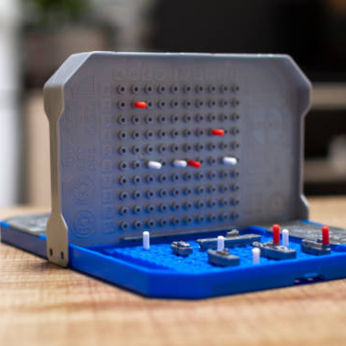
\includegraphics[width=0.7\textwidth]{figs/background/battleshipREAL.png}
    \end{minipage}
    \hfill % Crée l'espace entre les deux images
    % Deuxième image (droite)
    \begin{minipage}[H]{0.45\textwidth}
        \centering
        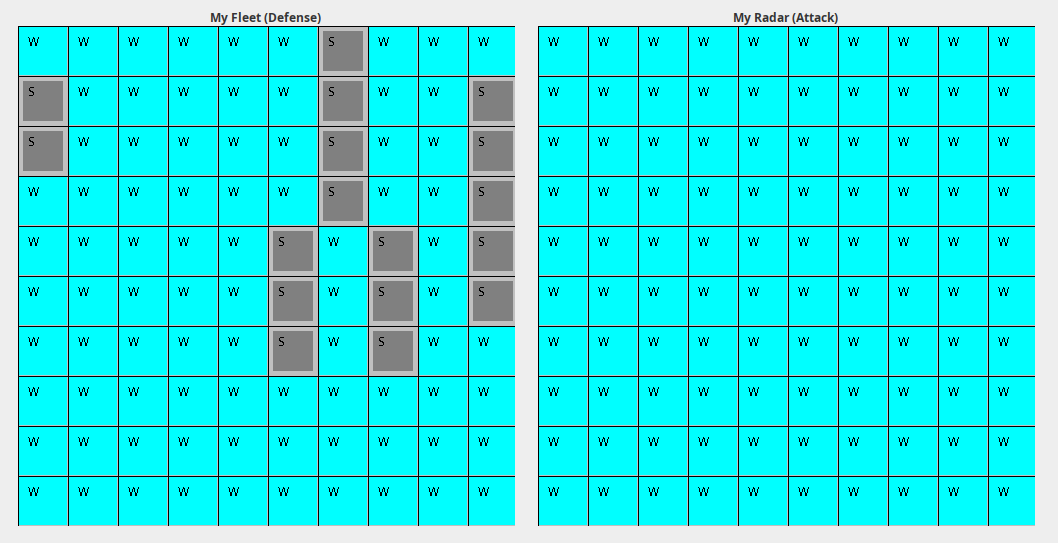
\includegraphics[width=1\textwidth]{figs/background/battleshipTAG.png}
    \end{minipage}

    \vspace{0.15cm} % Petit espace vertical avant la légende
    \captionsetup{justification=centering}
    \caption{Left: the physical Battleship board game. Right: the TAG graphical interface for the Battleship implementation developed in this thesis. The shot-tracking grid (right) records the acting player's observations; the ship grid (left) contains the true hidden fleet, masked from the opponent during play.}
    \label{fig:real_battleship_and_TAG_battleship}
\end{figure}

%%% 3.2 %%%
\section{Battleship Implementation in TAG}
\label{sec:battleship_tag_impl}

The Battleship benchmark was implemented in TAG using the standard three-component architecture described in Chapter~\ref{Background}. A game state class stores all information required to represent the current situation: separate ship grids and shot-tracking grids are maintained for each player. The ship grids contain the true hidden fleet configurations and are never exposed directly to the opposing agent; the shot-tracking grids store only the information revealed through previous actions, namely confirmed hits and misses. Remaining ship health values are maintained as auxiliary counters to allow the end-condition check to run in constant time rather than requiring a full grid scan at every move.

Game progression is handled by a forward model that generates all legal firing actions corresponding to untargeted cells on the opponent's grid. When an action is executed, both the hidden ship grid and the visible shot-tracking grid are updated according to the shot outcome. Hits and misses are therefore recorded incrementally as play progresses, continuously constraining the set of plausible opponent configurations available to the acting player. A separate parameter object stores the configurable properties of the game, including board dimensions and fleet composition, and is shared between the forward model and the determinization engine to ensure that all generated hypotheses remain consistent with the official game configuration.

The critical architectural contribution of this implementation lies not in the game logic itself but in how game-state copies are generated during simulations. In standard perfect-information environments, agents can safely reason over exact copies of the game state. In Battleship, directly copying the hidden opponent grid would expose privileged information during search. The state-copying mechanism therefore generates hypothetical hidden configurations consistent with the observations available to the requesting player, rather than simply duplicating the true state. The design of this mechanism is described in detail in the following section.


%%% 3.3 %%%
\section{Constraint-Based Determinization}
\label{sec:constraint_det}

The core contribution of the TAG benchmark lies in the determinization mechanism used during simulation-time state copying. Rather than exposing the true hidden opponent grid to search agents, the system generates hypothetical ship configurations that remain consistent with the observations available to the acting player.

The determinization process operates on two sources of information accumulated during gameplay. A \textit{hitMap} records every cell where the presence of an opponent ship has been confirmed through a successful shot. A \textit{missMap} records every cell where a shot has returned a negative result, confirming the absence of a ship. Together, these structures define a set of spatial constraints describing precisely which hidden configurations remain compatible with the player's accumulated observations. Figure~\ref{fig:det_pipeline} illustrates the overall pipeline from game observation to hypothesis generation.

\begin{figure}[H]
    \centering
    % TODO: Insert determinization pipeline diagram.
    % Suggested layout: left box "Player observations (hits + misses)" ->
    % arrow to center box "Constraint-Based Engine (CSP solver)" ->
    % arrow to right box "Coherent hypothesis (hypothetical grid)" ->
    % arrow down to "Injected into simulation copy"
    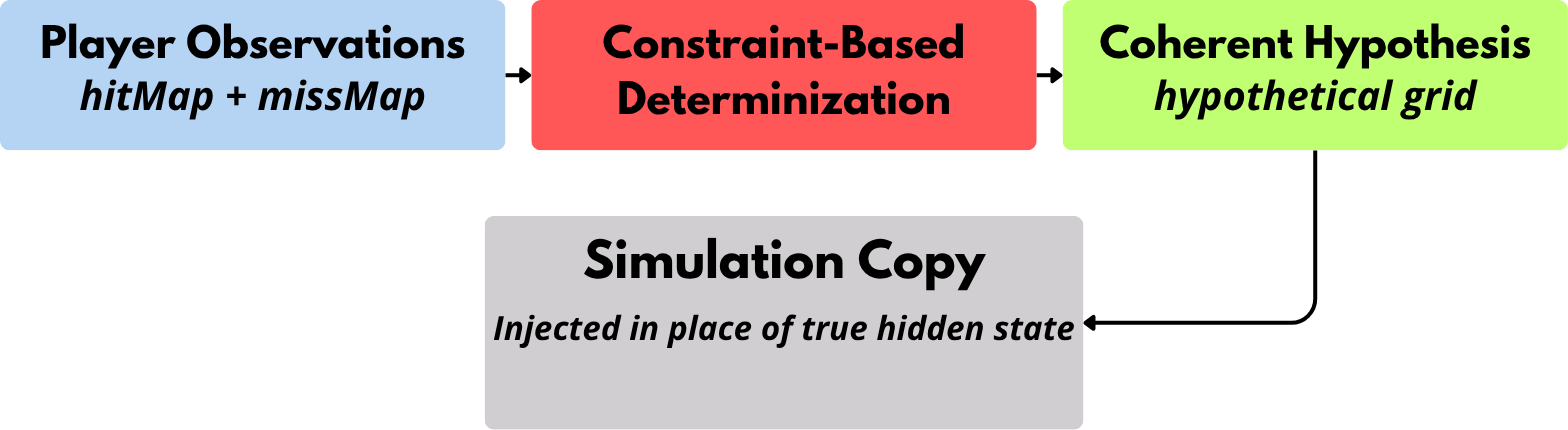
\includegraphics[width=1.00\textwidth]{figs/background/det_pipeline.png}
    \captionsetup{justification=centering}
    \caption{The constraint-based determinization pipeline. Accumulated hits and misses are used as spatial constraints to guide hypothesis generation. The engine produces a coherent hypothetical opponent grid that is injected into the simulation copy instead of the true hidden state.}
    \label{fig:det_pipeline}
\end{figure}

When a simulation copy is requested, the determinization engine constructs a hypothetical opponent grid satisfying these constraints. Ship placements conflicting with previously observed misses are rejected, while observed hits must remain covered by at least one valid ship placement. The generated hypothesis therefore represents a plausible hidden state consistent with the information available to the player at the time of the simulation.

The generation process can be interpreted as a constrained placement problem in which ships are placed sequentially. A placement is valid only if it remains within the board boundaries, does not overlap with any previously placed ship, and remains compatible with all entries in both the hitMap and the missMap. When multiple valid placements satisfy the current constraints, the engine samples among them in order to preserve diversity across simulations, preventing agents from repeatedly reasoning over a single deterministic hypothetical world. Figure~\ref{fig:det_example} illustrates an example of a coherent hypothetical configuration generated from partial observations.

\begin{figure}[H]
    \centering
    % TODO: Insert example of constraint-based determinization.
    % Suggested layout: 10x10 grid showing hit cells (red), miss cells (grey X),
    % and hypothesized ship placement (blue) consistent with all observations.
    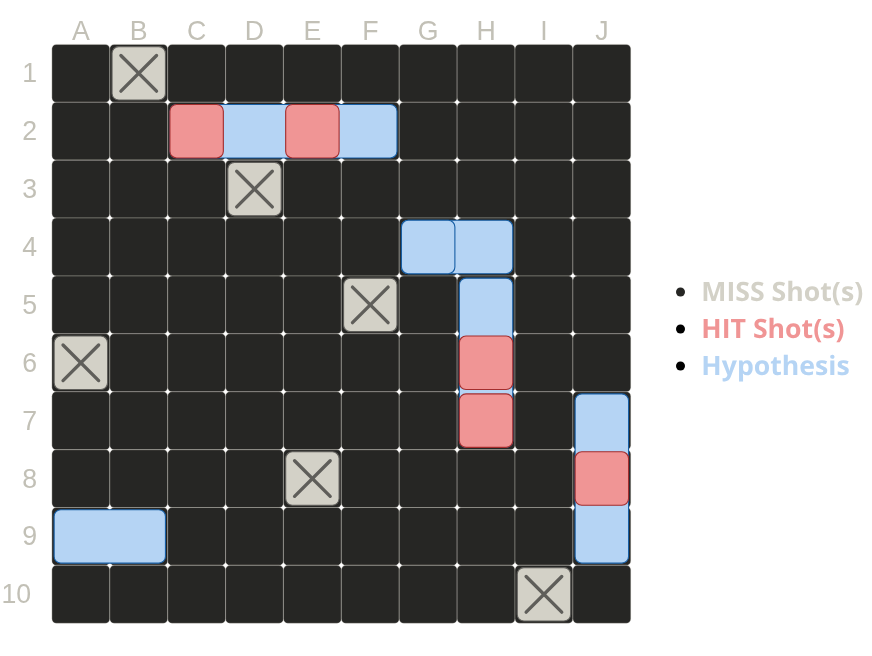
\includegraphics[width=0.65\textwidth]{figs/background/det_example.png}
    \captionsetup{justification=centering}
    \caption{Example of a constraint-based hypothetical configuration. Red cells are confirmed hits; grey cells are confirmed misses. The hypothesized fleet placement (blue) covers all hit cells and avoids all miss cells, representing one plausible world consistent with the agent's observations.}
    \label{fig:det_example}
\end{figure}

Unlike exact belief-state methods~\cite{morenville2024beliefsg,morenville2025belief_constraints}, the proposed approach does not attempt to enumerate or maintain the full distribution of possible hidden configurations. Instead, it approximates uncertainty through repeated generation of coherent hypothetical states during simulation. This makes the method computationally tractable while still preserving consistency with observed information. From a search perspective, the determinization engine acts as an intermediate layer between the true hidden game state and the simulation-based agent: the quality of the generated hypothetical states directly influences the quality of the forward simulations performed during search.


%%% 3.4 %%%
\section{Determinization Strategies}
\label{sec:det_strategies}

In order to evaluate the impact of hidden-state reconstruction quality on imperfect-information search, three determinization strategies were implemented in the TAG Battleship benchmark. Each strategy defines how hypothetical opponent ship configurations are generated during simulation-time state copying. The three approaches progressively increase the amount of information exploited from previous observations, making it possible to isolate the effect of increasingly informed determinization mechanisms while keeping the underlying search algorithms unchanged.

\subsection{Random Determinization}
\label{sec:random_det}

Random Determinization serves as the lower-bound baseline strategy. Hypothetical opponent ship configurations are generated through unconstrained random placement that respects only the structural rules of Battleship: board boundaries, ship sizes, orientations, and the non-overlap constraint. Hits and misses recorded during gameplay are entirely ignored when constructing the hypothetical opponent grid, so generated states may contradict information already revealed to the player, for instance by placing ships on cells previously observed as misses or by leaving known hit cells uncovered. This strategy therefore provides the worst-case reference for evaluating whether more informed determinizations improve simulation quality and, in turn, decision quality.

\subsection{Constraint-Based Determinization}
\label{sec:csp_det}

Constraint-Based Determinization incorporates the full set of observations accumulated during gameplay. The generated hidden configuration must remain consistent with all known hits and misses recorded in the player's shot-tracking grid. Cells marked as misses define forbidden positions; cells marked as hits must be covered by at least one ship in the generated hypothesis; all ships must additionally satisfy the standard placement constraints of remaining within the board, respecting their predefined lengths, and avoiding overlap with other ships.

Whenever several placements satisfy the current constraints, the engine samples among valid possibilities in order to preserve diversity across simulations. This allows agents to reason over multiple coherent hypothetical worlds rather than repeatedly reasoning from the same reconstructed configuration. The expected benefit of this strategy is improved simulation reliability: since the generated states no longer contradict previous observations, search algorithms evaluate actions in worlds that could plausibly correspond to the true hidden board, providing a genuine strategic signal rather than noise.

\subsection{Heatmap-Guided Determinization}
\label{sec:heatmap_det}

Heatmap-Guided Determinization extends the constraint-based strategy by estimating a probabilistic spatial prior over the opponent's grid. Rather than relying on a single coherent hypothesis per simulation copy, the engine first runs the constraint-based generator a large number of times to build a heatmap. Each sampled configuration contributes to this heatmap by incrementing a counter for every cell it occupies; the final heatmap is obtained by normalizing these counts over all samples. Cells with higher values correspond to locations that are more frequently occupied across the sampled configurations and therefore more likely to contain a ship according to the constraint-based prior.

This heatmap is then used to guide both determinization and action selection toward statistically plausible regions of the board. Rather than treating all constraint-consistent placements equally, the strategy weights sampling toward configurations that concentrate ships in high-probability zones, combining logical consistency with a lightweight approximation of the underlying belief distribution.

\begin{figure}[H]
    \centering
    % TODO: Insert heatmap visualization.
    % Suggested: 10x10 grid with a colour gradient from white (low probability)
    % to dark red (high probability), showing how probability concentrates
    % near known hit cells and around coherent ship-length continuations.
    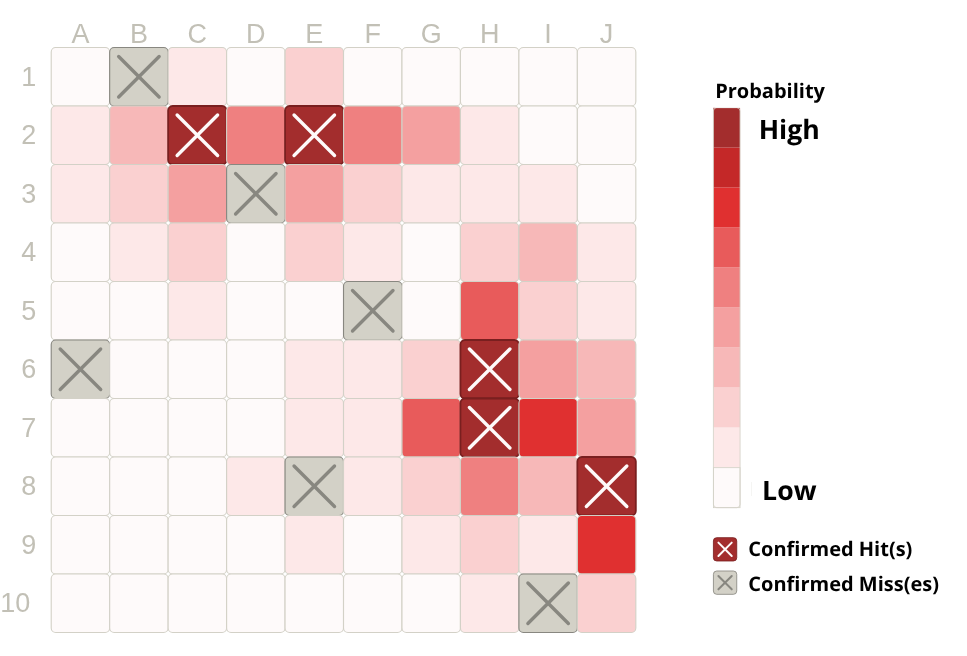
\includegraphics[width=0.7\textwidth]{figs/background/heatmap_example.png}
    \captionsetup{justification=centering}
    \caption{Example probabilistic heatmap produced by the Heatmap-Guided strategy after a partial game. Warmer colours indicate cells more frequently occupied across sampled constraint-consistent configurations. Probability concentrates near confirmed hit cells and along their plausible continuations.}
    \label{fig:heatmap_example}
\end{figure}



The central tradeoff of this strategy is computational cost. Building the heatmap requires running the constraint-based solver a large number of times before each decision, substantially increasing the time required to produce a simulation-ready copy of the game state. Agents that rely heavily on generating many simulations within a fixed time budget may therefore afford fewer iterations per move under this strategy, potentially offsetting the benefit of higher-quality individual simulations. The experiments in Section~\ref{sec:results} quantify this tradeoff directly.


%%% 3.5 %%%
\section{Experimental Setup}
\label{sec:exp_setup}

This section describes the experimental protocol used to evaluate the impact of determinization quality on simulation-based agents in the TAG Battleship benchmark. The experiments were designed to compare the three strategies introduced in Section~\ref{sec:det_strategies} while keeping the underlying search algorithms and game environment unchanged.

\subsection{Tournament Protocol}

The evaluation follows a round-robin tournament format in which every pair of agents competes in both player positions. For each matchup, agents alternate between playing first and second in order to control for first-player bias effects. Battleship is particularly sensitive to turn order because the first player always obtains the first opportunity to fire, accumulating hit and miss information one step ahead of the opponent. Each matchup consists of 100 games per direction, for a total of 200 games per pair, and the experiments are repeated independently for each of the three determinization strategies. This protocol makes it possible to isolate the impact of the determinization mechanism itself while preserving identical gameplay conditions across all comparisons.

\subsection{Evaluated Agents}

The benchmark evaluates five simulation-based agents representative of common General Game Playing approaches. The \textbf{Random} agent selects legal actions uniformly at random and never queries the game state, making it the primary control for validating that performance differences are genuinely attributable to determinization quality. \textbf{OSLA} applies a one-step lookahead heuristic, evaluating each legal action through a single forward simulation and selecting the highest-scoring immediate outcome. \textbf{RMHC} maintains a rolling horizon of candidate action sequences and optimizes them through repeated random mutation, relying on many forward simulations per decision step. \textbf{IS-MCTS} builds a search tree across multiple determinizations by sampling a new hypothetical world at each simulation step, aggregating results to identify the best action. \textbf{MAST} extends IS-MCTS by maintaining move-average statistics across rollouts to bias action selection toward historically effective moves.

Each agent is evaluated under all three determinization strategies, and search-based agents are additionally run under three thinking-time budgets of 100\,ms, 500\,ms, 1000\,ms and 5000\,ms per move. This multi-budget design allows the interaction between computational resources and determinization quality to be studied, in particular whether additional simulation time amplifies or compensates for the differences between strategies.

\subsection{Evaluation Metrics}

The experiments measure both gameplay performance and computational behavior in order to characterize the full impact of each determinization strategy.

The primary gameplay metric is win rate: the fraction of games won by an agent across all its matchups under a given strategy. As a secondary gameplay metric, the remaining ship health difference at the end of each game is recorded to assess how dominant or competitive individual matches are, providing a finer-grained view of agent strength than win rate alone.

On the computational side, three metrics are tracked for each strategy. Copy latency measures the average time in nanoseconds required to produce a single simulation-ready game-state copy, capturing the overhead introduced by the constraint solver relative to a raw copy. Search effort counts the average number of ship-placement attempts required by the engine before a valid constraint-consistent configuration is found, reflecting the difficulty of the constraint satisfaction problem as a function of game progression. Finally, the determinization success rate records the proportion of copy calls that result in a fully coherent hypothesis rather than a fallback to unconstrained random placement, validating the robustness of the constraint-based and heatmap-guided implementations as the game advances and the constraint set grows.

Together, these metrics make it possible to study not only whether informed determinizations improve agent performance, but also the computational tradeoffs they introduce.

\newpage

%%% 3.6 %%%
\section{Experimental Results}
\label{sec:results}

This section presents the experimental results obtained on the TAG 
Battleship benchmark. All experiments were conducted on the Dragon2 
computing cluster at UCLouvain. The cluster consists of 17 computing 
nodes, each equipped with two Intel Skylake Xeon 6142 processors 
(16 cores, 2.6 GHz); 15 nodes have 192 GB of RAM and 2 nodes have 
384 GB, all with 3.3 TB of local scratch space. Two additional nodes 
equipped with two Intel Skylake Xeon 6126 processors (12 cores, 
2.6 GHz) each host two NVIDIA Tesla V100 GPUs (5120 CUDA cores, 
16 GB HBM2, 7.5 TFlops double precision).%
\footnote{Full hardware specifications are available at the CÉCI 
documentation: \url{https://www.ceci-hpc.be/clusters/dragon2/}}

\subsection{Overall Agent Performance}
\label{subsec:overall}

The first set of experiments evaluates the overall win rates achieved 
by each agent under the three determinization strategies. 
Table~\ref{tab:winrates} summarizes the results across all agent and 
strategy combinations.

\begin{table}[H]
\centering
\begin{tabular}{lccc}
\hline
\textbf{Agent} & \textbf{Random Det.} & \textbf{Constraint-Based Det.} 
               & \textbf{Heatmap-Guided Det.} \\
\hline
Random  & $\approx 44\%$ & $\approx 2\%$  & $\approx 2\%$  \\
OSLA    & $\approx 53\%$ & $\approx 87\%$ & $\approx 87\%$ \\
RMHC    & $\approx 53\%$ & $\approx 87\%$ & $\approx 87\%$ \\
IS-MCTS & $\approx 49\%$ & $\approx 37\%$ & $\approx 37\%$ \\
MAST    & $\approx 50\%$ & $\approx 38\%$ & $\approx 37\%$ \\
\hline
\end{tabular}
\captionsetup{justification=centering}
\caption{Average win rates by agent and determinization strategy 
         (1000\,ms budget, rounded).}
\label{tab:winrates}
\end{table}

The results reveal a striking and consistent pattern. Under Random 
Determinization, all five agents perform near chance level, with win 
rates ranging from 44\% to 53\%. While small deviations from 50\% are 
visible, notably OSLA and RMHC at 53\% and Random at 44\%, no 
agent demonstrates meaningful strategic advantage at this stage. 
IS-MCTS, which builds a search tree through repeated simulations, 
achieves the same result as the Random agent, which picks actions 
blindly. This uniformity is not surprising: it is exactly the outcome 
that Random Determinization was designed to demonstrate. Because each 
simulation is performed in a world where ships are placed with no 
regard for observed hits and misses, the resulting action evaluations 
carry no information about the true hidden configuration. Aggregating 
many such simulations, as IS-MCTS does, only produces a more confident 
wrong answer. The principle is simple: garbage in, garbage out.

The transition to Constraint-Based Determinization produces an 
immediate and dramatic reversal. OSLA and RMHC emerge as the strongest 
agents, achieving win rates of approximately 87\%. The Random agent, 
as expected, shows no improvement: since it never consults the game 
state to make decisions, the quality of the copy it receives is 
entirely irrelevant to its behavior. This invariance of the Random 
agent across all three strategies serves as a critical sanity check, 
confirming that the observed performance differences in other agents 
are genuinely caused by the determinization mechanism rather than by 
any confounding factor in the experimental setup.

\begin{figure}[H]
    \centering
    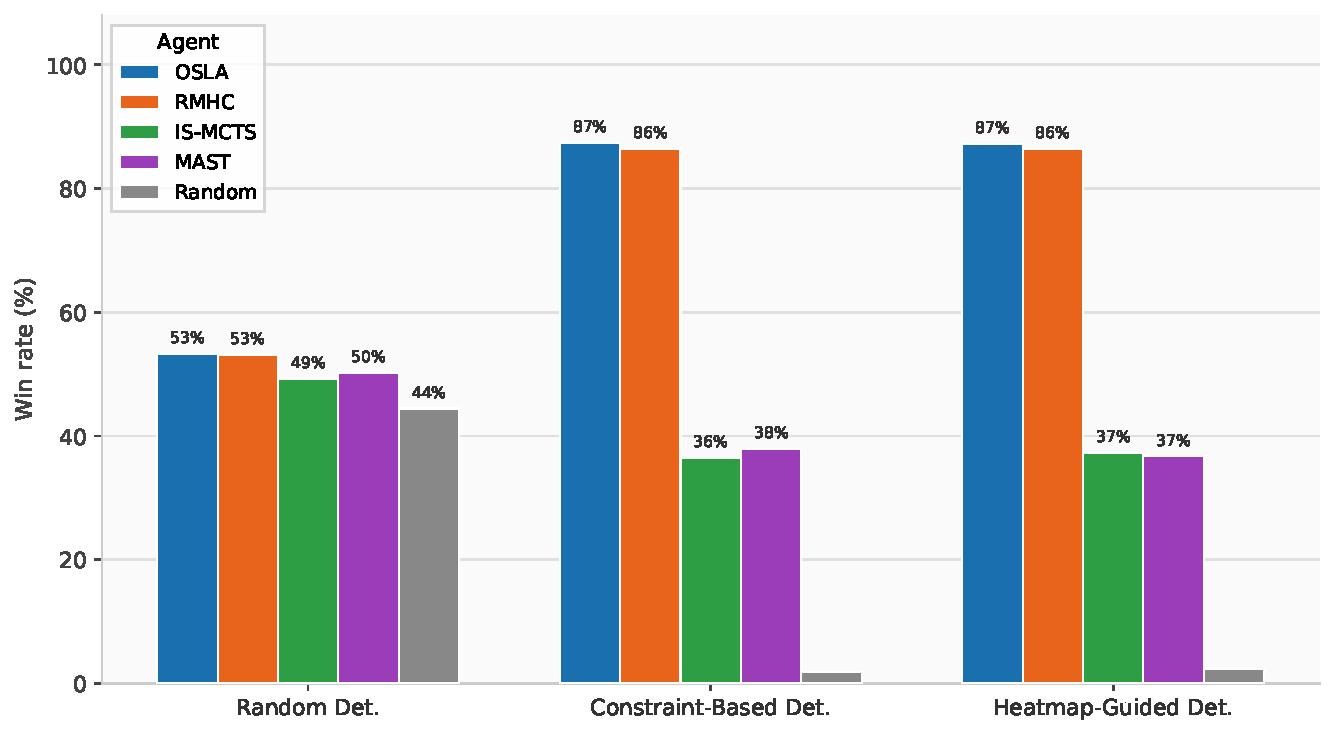
\includegraphics[width=1\textwidth]{Sections/4_TAG/figs/winrate_barplot.pdf}
    \captionsetup{justification=centering}
    \caption{Average win rates per agent under the three determinization 
    strategies (1000\,ms budget).}
    \label{fig:winrate_barplot}
\end{figure}

The strong performance of OSLA under Constraint-Based Determinization 
is particularly noteworthy, given that it only looks one step ahead. 
When that single forward step is simulated in a world that is logically 
consistent with the observed game history, the heuristic evaluation 
becomes meaningful: the agent can reliably distinguish between targeting 
a cell near a confirmed hit and targeting a region already identified as 
empty. This is precisely the spatial reasoning that constraint-based 
filtering enables, and it allows even a shallow agent to make 
well-informed decisions. The results suggest that in imperfect-information 
environments with structured spatial uncertainty, simulation consistency 
matters more than search depth. IS-MCTS and MAST, by contrast, achieve win rates of approximately 37\% under Constraint-Based Determinization which is lower than under Random Determinization. This apparent paradox is explained by the tournament 
structure: OSLA and RMHC now dominate every matchup so decisively that 
IS-MCTS and MAST lose the majority of their games against them. 

\newpage

\begin{figure}[H]
    \centering
    
    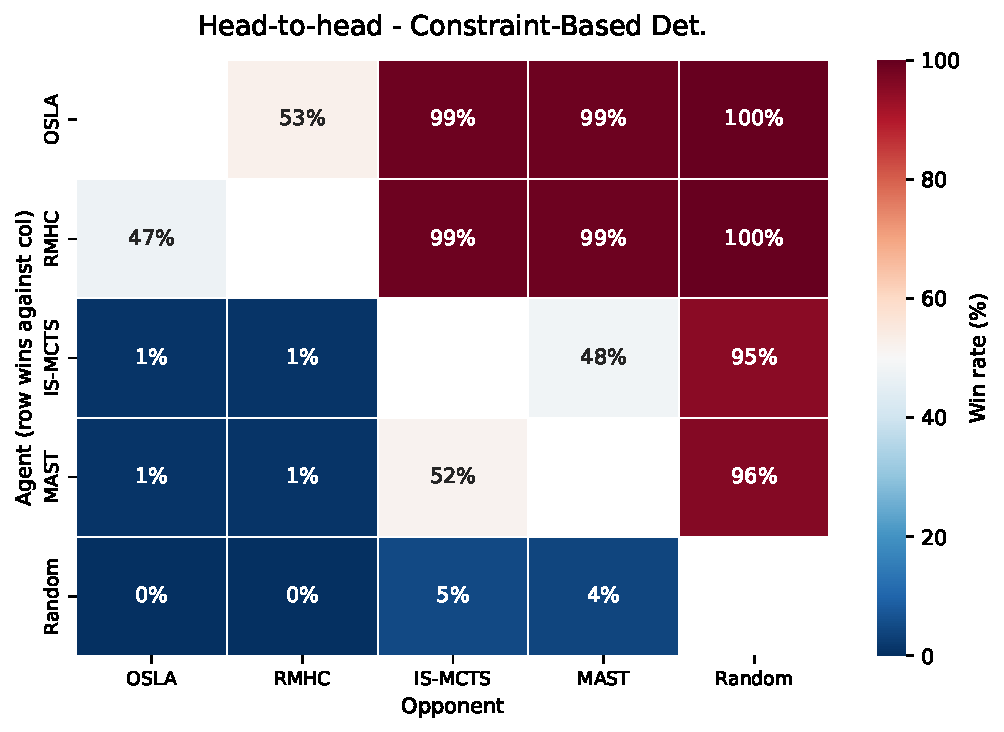
\includegraphics[width=\textwidth]{Sections/4_TAG/figs/heatmap_constraintbased_det.pdf}
    
    \vspace{0.3cm}
    
    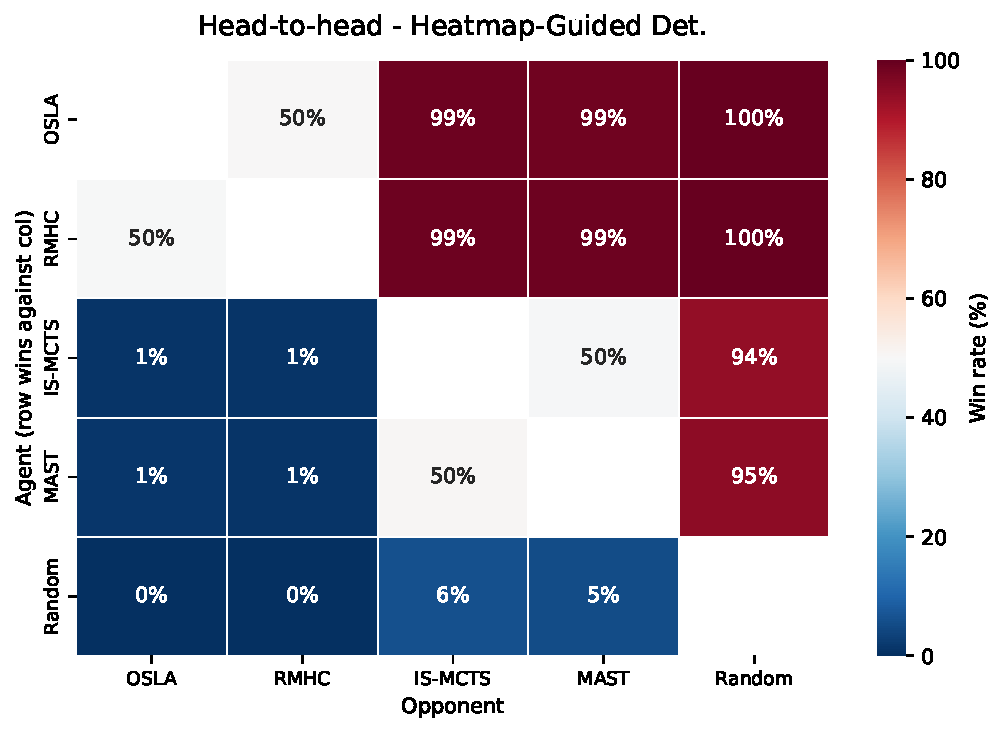
\includegraphics[width=\textwidth]{Sections/4_TAG/figs/heatmap_heatmapguided_det.pdf}
    
    \vspace{0.15cm}
    \captionsetup{justification=centering}
    \caption{Head-to-head win rates under Constraint-Based (top) and 
    Heatmap-Guided (bottom) Determinization (1000\,ms budget). 
    OSLA and RMHC dominate every matchup against IS-MCTS and MAST 
    under both strategies, and the pairwise patterns are 
    indistinguishable, confirming that the heatmap provides no 
    measurable advantage in head-to-head outcomes at this time budget.}
    \label{fig:heatmap_both}
\end{figure}

In direct matchups, OSLA wins over 98\% of its games against IS-MCTS. The 
constraint-based hypotheses benefit OSLA and RMHC directly at each 
evaluation step, whereas IS-MCTS still performs its rollouts using 
uniform random target selection. A deeper search tree built over coherent 
worlds provides limited benefit when the terminal evaluations are guided 
by random play.

Under Heatmap-Guided Determinization, no agent shows a meaningful 
change relative to Constraint-Based Determinization. OSLA and RMHC 
maintain their win rates near 87\%, while IS-MCTS and MAST remain near 
37\% regardless of the number of heatmap sampling iterations used 
(10, 50, or 100). The heatmap therefore provides no measurable 
performance benefit in this experimental setting. One possible explanation 
is that the heatmap improves the spatial prior used during 
determinization, but does not address the fundamental limitation of 
IS-MCTS and MAST: their rollout policies remain uniform random, so the 
quality of individual simulations is not improved by a more informed 
prior over ship positions.

The head-to-head matrices confirm this pattern at the pairwise 
level: under Constraint-Based and Heatmap-Guided Determinization, 
OSLA and RMHC win over 99\% of their games against IS-MCTS and 
MAST, while Random loses virtually all matchups against the 
stronger agents.

\newpage

\subsection{Impact of Computational Budget}
\label{subsec:budget}

The second set of experiments studies how performance evolves as the 
thinking-time budget increases from 100\,ms to 500\,ms, 1000\,ms, and 
5000\,ms, under both Constraint-Based and Heatmap-Guided Determinization.

\begin{figure}[H]
    \centering
    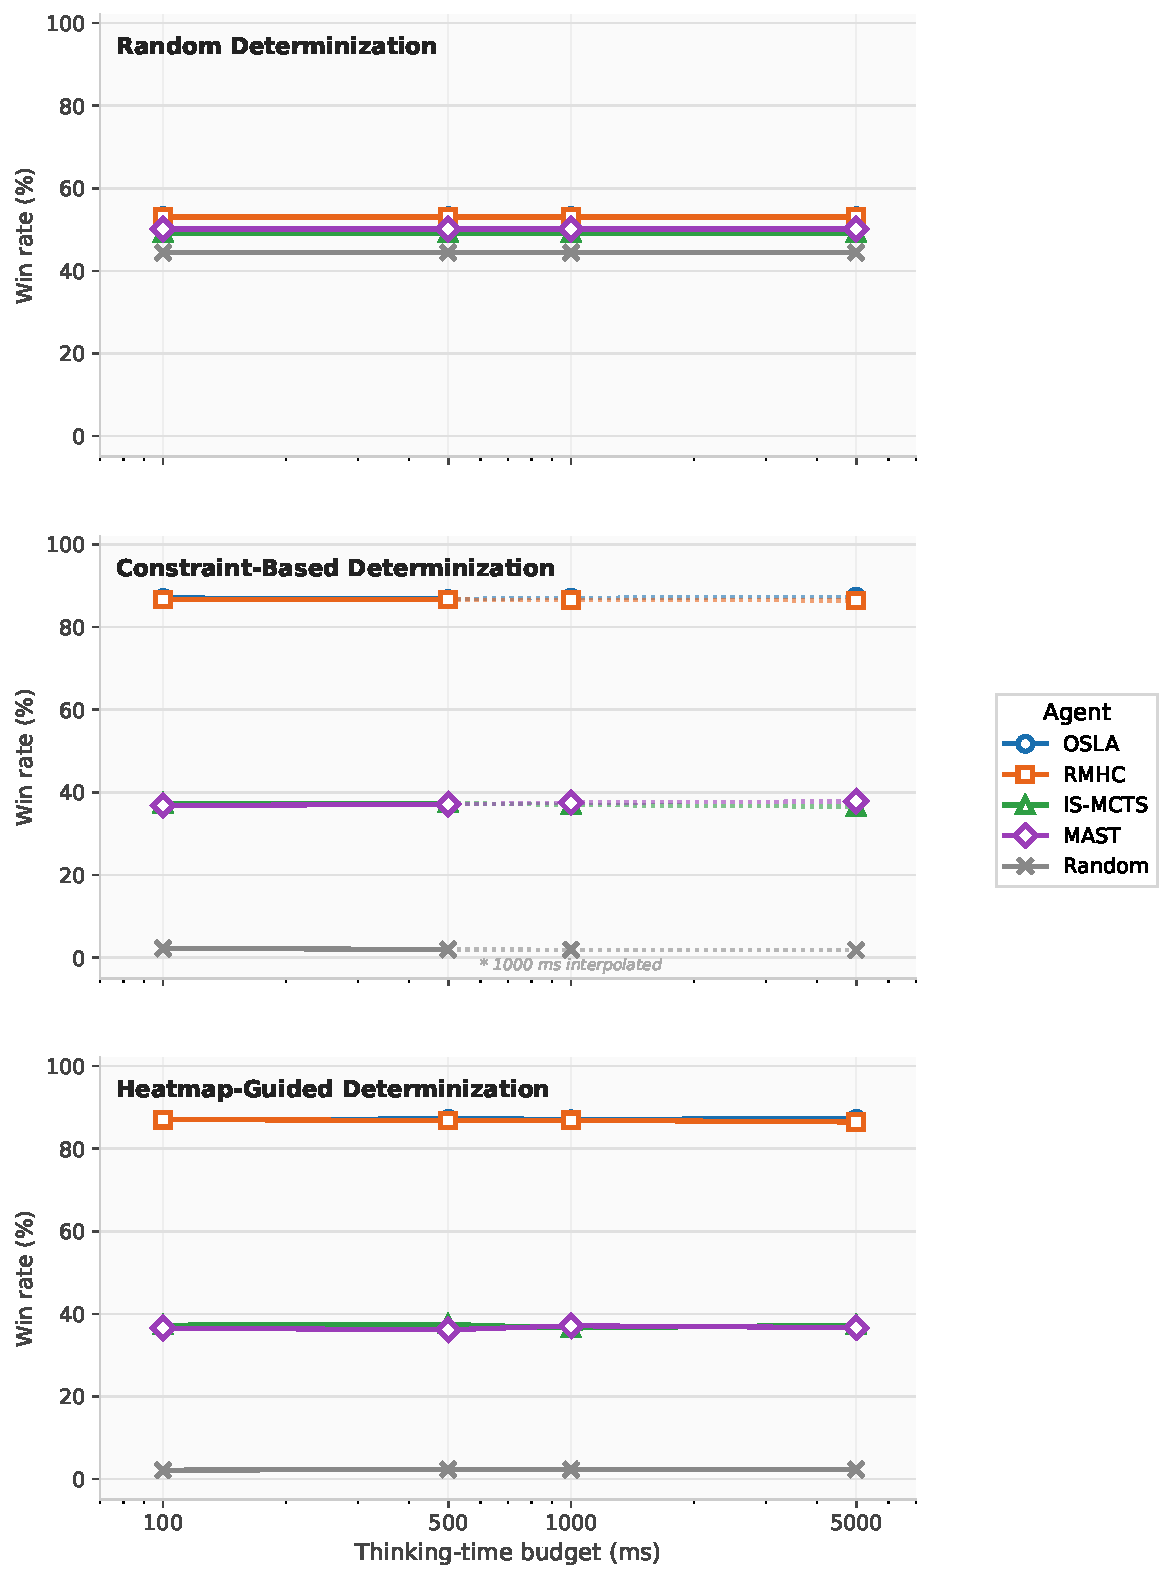
\includegraphics[width=0.9\textwidth]{Sections/4_TAG/figs/winrate_vs_time.pdf}
    \captionsetup{justification=centering}
    \caption{Win rate as a function of thinking-time budget for each 
    agent under the three determinization strategies. Color identifies 
    the agent; line style identifies the strategy. Under all strategies, 
    no agent shows a meaningful performance change as the budget 
    increases from 100\,ms to 5000\,ms.}
    \label{fig:winrate_vs_time}
\end{figure}

The results are unambiguous: the budget has no measurable effect on 
agent performance under any strategy. OSLA and RMHC maintain win rates 
of approximately 87\% across all four time budgets, and IS-MCTS and 
MAST remain near 37\% regardless of how much additional computation 
time they receive.

This invariance is itself an informative result. For OSLA, the absence 
of a budget effect is expected: since it evaluates only a single forward 
step per action, additional time beyond the minimum required to assess 
all legal moves provides no benefit. For IS-MCTS and MAST, the result 
is more significant: more simulation time does not compensate for the 
structural limitation of random rollouts. Building a deeper search tree 
over constraint-consistent worlds still produces unreliable value 
estimates if the terminal evaluations are guided by uniform random play. 
This confirms that the bottleneck for these agents is not computational 
budget but rollout quality.

\subsection{Game Outcome Analysis}
\label{subsec:outcomes}

Beyond win rates, the experiments also characterise the nature and 
margin of game outcomes across the three determinization strategies.

\begin{figure}[H]
    \centering
    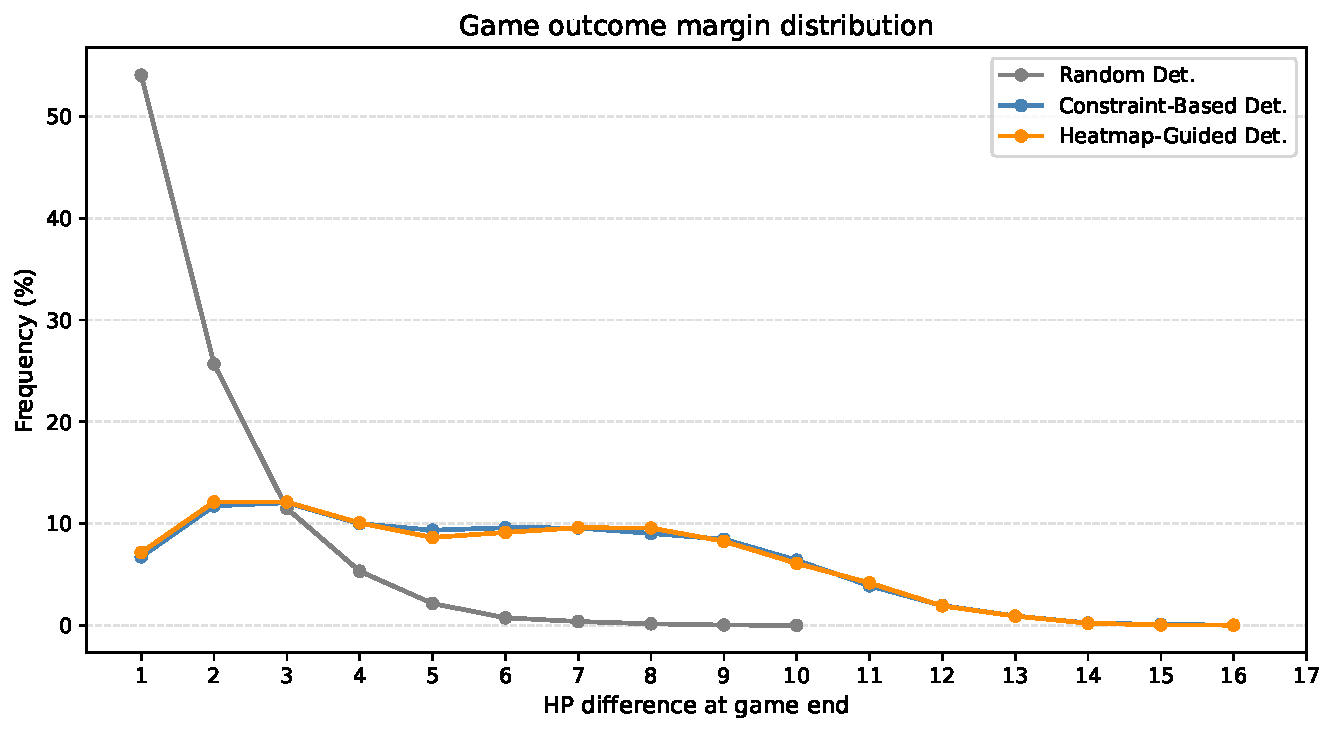
\includegraphics[width=\textwidth]{Sections/4_TAG/figs/drama_distribution.pdf}
    \captionsetup{justification=centering}
    \caption{Distribution of the HP difference between winner and loser 
    at the end of each game, shown for all three determinization strategies. 
    Under Random Determinization, the majority of games end with a margin 
    of 1 HP; under Constraint-Based and Heatmap-Guided Determinization, 
    the distribution flattens toward larger margins (1000ms budget).}
    \label{fig:drama}
\end{figure}

Figure~\ref{fig:drama} characterises the nature of game outcomes across 
strategies. Under Random Determinization, the majority of games end with 
a margin of just 1\,HP, indicating closely contested matches in which 
neither agent holds a consistent advantage. Under Constraint-Based and 
Heatmap-Guided Determinization, the distribution flattens and shifts 
toward larger margins, with many games ending with differences of 
5\,HP or more.

The winner's remaining HP distribution tells the same story from the 
other side: winners under Constraint-Based and Heatmap-Guided 
Determinization finish with substantially more HP than under Random 
Determinization, reflecting the fact that informed agents do not merely 
win more often, they win more decisively. This result is consistent 
with the head-to-head analysis: when OSLA or RMHC faces IS-MCTS or the 
Random agent under an informed strategy, the outcome is rarely close. 
The combination of coherent simulation hypotheses and direct spatial 
exploitation at each evaluation step produces a systematic and 
one-sided advantage.

\begin{figure}[H]
    \centering
    
    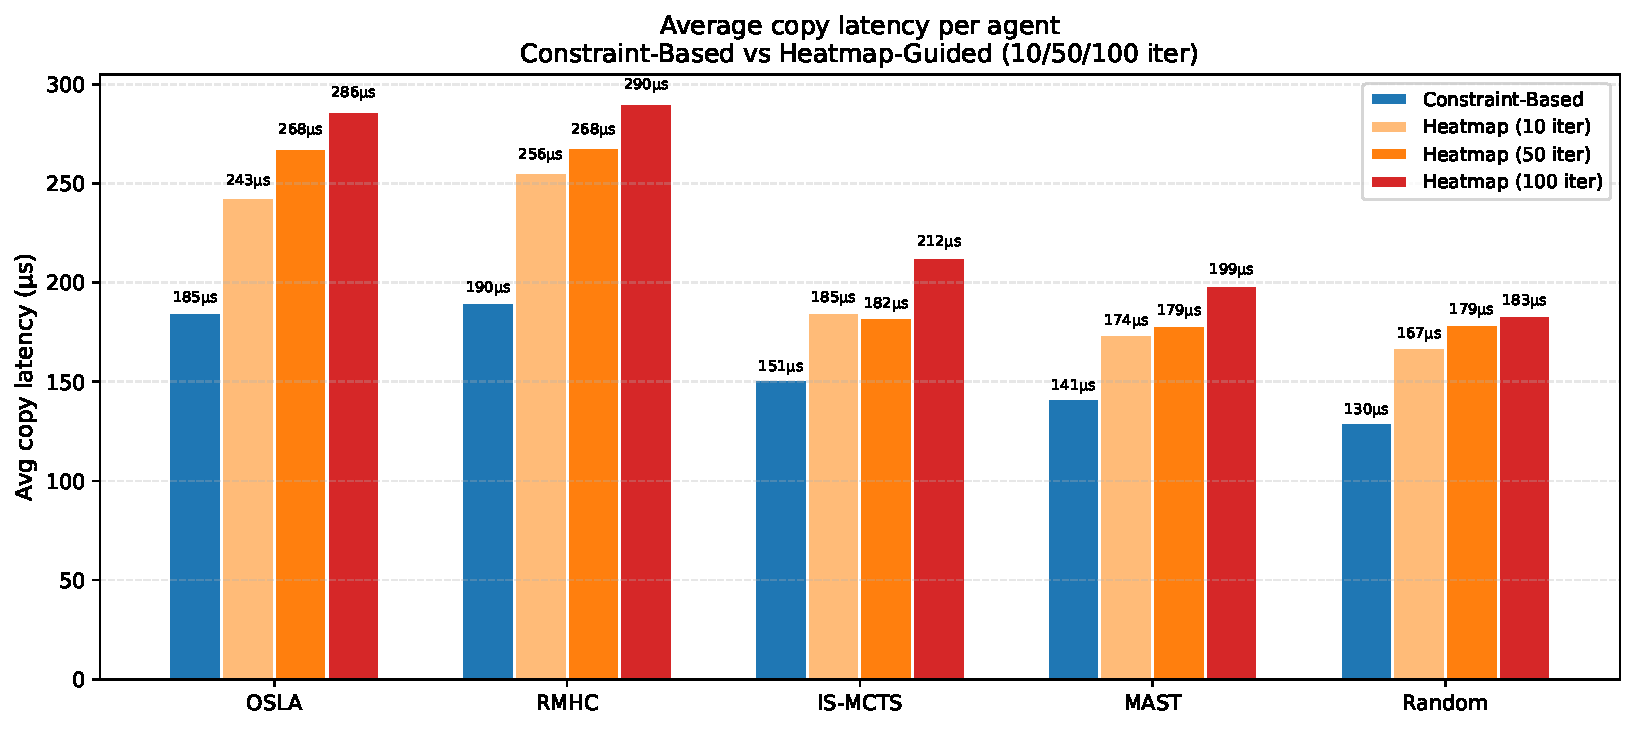
\includegraphics[width=\textwidth]{Sections/4_TAG/figs/copy_latency.pdf}
    
    \vspace{0.3cm}
    
    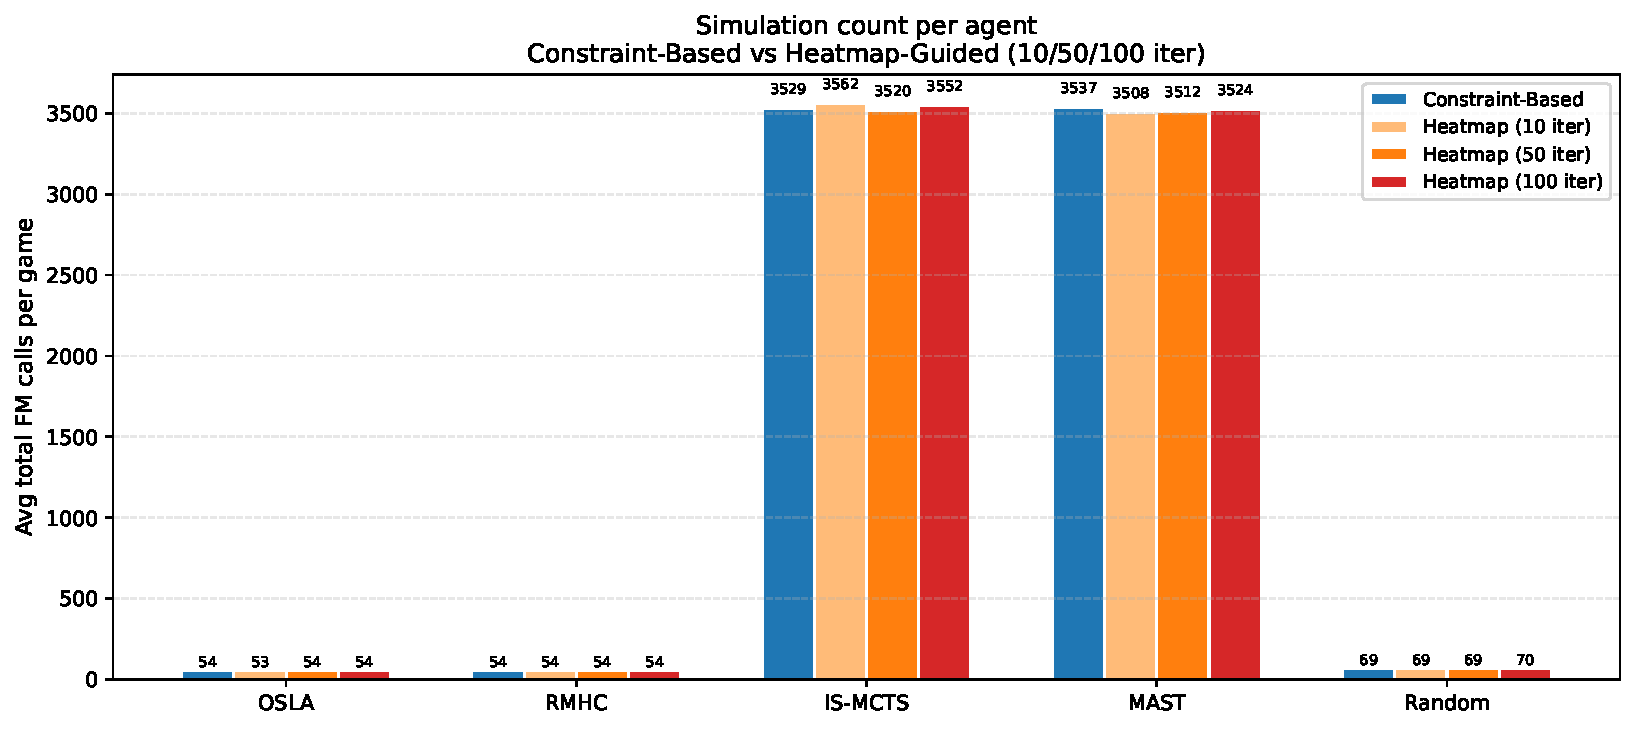
\includegraphics[width=\textwidth]{Sections/4_TAG/figs/fm_calls.pdf}
    
    \vspace{0.15cm}
    \captionsetup{justification=centering}
    \caption{Average copy latency (top) and total forward model calls per game 
    (bottom) for Constraint-Based and Heatmap-Guided Determinization 
    (10, 50, and 100 heatmap iterations). Despite a higher copy latency under Heatmap-Guided Determinization, the number of forward model calls remains comparable across all strategies.}
    \label{fig:copy_latency_and_fm_calls}
\end{figure}

Figure~\ref{fig:copy_latency_and_fm_calls} 
confirms that the budget invariance is not due to insufficient 
simulation depth. Despite Heatmap-Guided Determinization 
introducing a copy latency approximately 55\% higher than 
Constraint-Based, the total number of forward model calls per 
game remains comparable across both strategies, indicating that 
the 1000\,ms budget absorbs the overhead without reducing 
simulation count.


%%% 3.7 %%%
\section{Discussion}
\label{sec:tag_discussion}

The experiments conducted on the TAG Battleship benchmark highlight the central importance of determinization quality in imperfect-information simulation-based search. The results suggest that simulation consistency plays a more decisive role than search algorithm sophistication in hidden-information environments. Random Determinization frequently generates hypothetical states that contradict previously observed information, forcing search algorithms to reason over implausible worlds and producing no useful strategic signal regardless of how many simulations are run. Constraint-Based Determinization restricts simulations to configurations compatible with known hits and misses, producing search trajectories that accurately reflect the uncertainty actually faced by the player and enabling even shallow agents such as OSLA to perform strongly. The Heatmap-Guided strategy further refines this process by weighting simulations toward statistically plausible regions of the board, providing an additional benefit for tree-search agents at the cost of increased per-copy computational overhead.

The experiments also reveal an important observation about the relationship between determinization quality and the search algorithm. One might expect that a more powerful algorithm such as IS-MCTS, which samples many worlds and aggregates their results, would be more robust to poor determinizations than a shallow agent like OSLA. The results show the opposite: under Random Determinization, IS-MCTS performs no better than the Random agent, while OSLA achieves strong performance as soon as the determinizations become constraint-consistent. Aggregating many incoherent simulations does not produce a useful signal; it merely produces a more confident wrong answer. The gains from more sophisticated search are therefore contingent on the quality of the hypothetical worlds those algorithms reason about.

Another observation concerns the independence between the determinization mechanism and the search algorithm. The same agent exhibits substantially different behavior depending on the quality of the hypothetical states it receives during simulation. This reinforces one of the central claims of this thesis: in imperfect-information environments, hidden-state reconstruction is a fundamental component of the simulation architecture rather than a secondary implementation detail. Improving determinization quality is a more reliable path to better agent performance than increasing search depth, at least in the hidden-position setting studied here.

More broadly, the TAG implementation demonstrates that preserving uncertainty during simulation-time state copying can significantly improve imperfect-information reasoning while remaining compatible with general simulation-based search techniques. The benchmark therefore provides a useful reference architecture for studying hidden-information handling in General Game Playing systems. These observations directly motivate the next part of this thesis: while TAG enables explicit control over player-specific state copying through its code-first architecture, Ludii currently relies on more generic context-copy mechanisms. The following chapters investigate how determinization techniques inspired by this benchmark can be integrated into Ludii in order to preserve hidden-information uncertainty during simulation-based search.
\chapter{Hidden-Information Simulation in Ludii}
\label{HiddenInfoSimulationLudii}

\begin{abstract}
The previous chapter demonstrated that preserving uncertainty during simulation-time state copying can significantly influence the behavior and performance of simulation-based agents in imperfect-information environments. In TAG, this was achieved through explicit control over player-specific game-state copies and determinization mechanisms integrated directly into the game implementation.

This chapter investigates how hidden-information simulations are currently handled in Ludii. Although Ludii provides extensive support for imperfect-information game representation at the language level, simulation-based search relies on generic runtime mechanisms that were originally designed primarily for perfect-information environments.

The objective of this chapter is therefore to analyze the interaction between hidden-information games and Ludii's simulation architecture. Particular attention is given to how \textsc{Context} objects are copied during search and how unrestricted copies expose privileged information to agents during forward simulation.

The chapter first presents the Battleship implementation in Ludii and examines how hidden information is represented internally. It then analyzes the behavior of simulation-time context copying and demonstrates why visibility constraints enforced during normal gameplay are not sufficient to preserve uncertainty during AI search. An empirical tournament then quantifies the impact of this information leakage. These observations motivate the determinization mechanisms introduced in the following chapter.
\end{abstract}

\section{Battleship in Ludii}
\label{sec:battleship_ludii}

Battleship is available in the Ludii library as \textsc{Battleships.lud}. As with all games in Ludii, the game rules, equipment, and hidden-information structure are declared entirely within this file using the Ludii Game Description Language, without any game-specific Java code.

The game is played on two separate $10 \times 10$ grids, one per player. Each player's grid is divided into two regions declared in the \textsc{.lud} file: a \textit{Defence} region, where the player's own fleet is placed at the start of the game, and an \textit{Attack} region, which records shots fired at the opponent. Five ships of sizes 5, 4, 3, 3, and 2 are placed on the Defence region before play begins. Players then alternate firing shots at the opponent's Attack grid; each shot is answered with a hit or miss result. The player who sinks the entire opponent fleet first wins.

Hidden information is declared directly in the game description using the \texttt{set Hidden} ludeme:

\begin{center}
    \begin{verbatim}
        (set Hidden (sites P1 "Defence") to:P2)
        (set Hidden (sites P2 "Defence") to:P1)
    \end{verbatim}
\end{center}

This instructs Ludii that each player's Defence region is invisible to the opponent. During normal gameplay and in the graphical interface, Ludii correctly enforces this constraint: a human player sees only their own fleet and the results of their shots. The hidden ships are never displayed to the opposing side.

At the level of the game description, Battleship in Ludii is therefore a correct and well-formed imperfect-information game. The problem studied in this chapter concerns not how hidden information is \emph{declared}, but how it is \emph{handled} when simulation-based AI agents copy the game state during search.

%%% 4.2 %%%
\section{Simulation-Time Context Copying}
\label{sec:copycontext}

\subsection{The \textsc{copyContext()} Mechanism}

Simulation-based agents in Ludii evaluate future actions by repeatedly copying the current game state and performing forward simulations on these copies. This process is mediated by the \textsc{copyContext()} method defined in \textbf{AI.java}, the base class for all Ludii agents. At each decision point, an agent calls \textsc{copyContext()} to obtain a working copy of the current \textsc{Context} on which it can safely simulate without affecting the real game.

As described in Chapter~\ref{Background}, the \textsc{Context} object contains the complete internal state of the game, including the \textsc{State} substructure, which stores all cell-level information, and the \textsc{Trial} substructure, which records the history of moves. Each cell on the board is represented internally as a \textit{chunk}: a compact data structure that stores, among other things, a \texttt{who} field indicating which player owns the piece on that cell, and a \texttt{what} field indicating the type of that piece.

The implementation of \textsc{copyContext()} performs a direct copy of the \textsc{Context} object. All chunk values are duplicated as-is for every cell on the board, including cells that belong to hidden regions. No filtering, masking, or randomization is applied to the copied state.

\subsection{The Information Leakage Problem}

The consequence of this raw copying behavior is straightforward but significant. When a simulation-based agent calls \textsc{copyContext()} during search in a Battleship game, the copy it receives contains the complete and unmodified \textsc{State}, including the \texttt{who} and \texttt{what} values of every cell in the opponent's Defence region. The agent therefore has access, through the copied context, to the exact positions of all opponent ships, even cells it has never targeted.

This is not intentional cheating on the part of the agent. The agent simply evaluates moves on the copy Ludii provides, and that copy happens to contain information it should not see. From the agent's perspective, it is reasoning about a hypothetical future, but the hypothetical state is in fact the true game state with no information withheld.

The contrast with TAG is sharp. In TAG, \textsc{\_copy(playerID)} is called with a player identifier, and the game implementation controls precisely what the copy contains. Hidden pieces are replaced by hypotheses or randomized configurations before the agent ever sees them. In Ludii, no such mechanism exists: \textsc{copyContext()} is player-agnostic and exposes the full underlying state unconditionally.

\subsection{Where the Problem Lives in the Architecture}

The root cause is architectural rather than accidental. Ludii was designed primarily for perfect-information games, where unrestricted state copies are both safe and desirable. The \textsc{Context} object was never intended to act as a player-specific observation; it is a complete world representation. The \texttt{set Hidden} ludeme correctly controls what the graphical interface renders and what moves are listed as legal, but it has no effect on what \textsc{copyContext()} returns to a search algorithm.

Table~\ref{tab:arch_comparison} summarizes the key architectural differences between TAG and Ludii with respect to hidden-information handling during simulation.

\begin{table}[H]
\centering
\begin{tabular}{lll}
\hline
 & \textbf{TAG} & \textbf{Ludii} \\
\hline
Game logic & Java (\texttt{AbstractForwardModel}) & \textsc{.lud} file (ludemes) \\
Game state & \texttt{AbstractGameState} & \texttt{Context} \\
Agent API & \texttt{\_getAction()} & \texttt{selectAction()} \\
Copy mechanism & \texttt{\_copy(playerID)} & \texttt{copyContext()} \\
Copy is player-aware & Yes & No \\
Hidden info in copy & Masked / replaced & Fully exposed \\
\hline
\end{tabular}
\caption{Architectural comparison of hidden-information handling during simulation in TAG and Ludii.}
\label{tab:arch_comparison}
\end{table}

Any simulation-based Ludii agent that calls \textsc{copyContext()} in an imperfect-information game therefore operates, unknowingly, with complete knowledge of the hidden state. The degree to which this inflates agent performance depends on the game: in Battleship, where the entire opponent fleet is hidden, the effect is maximal.


%%% 4.3 %%%
\section{Experimental Characterization of Information Leakage}
\label{sec:leakage_experiment}

\subsection{Experimental Setup}

To empirically quantify the impact of this information leakage, a controlled tournament was conducted in Ludii using native agents with no modification to their copy mechanism. The tournament follows the same round-robin format used in Chapter~3: every pair of agents plays 100 games in each direction, for a total of 200 games per matchup. All agents were evaluated under identical time conditions using the default configuration of the Ludii evaluation framework.

Four native Ludii agents were evaluated:
\begin{itemize}
    \item \textbf{Random}: selects a legal action uniformly at random, never calling \textsc{copyContext()}.
    \item \textbf{UCT}: MCTS with UCB1 tree selection~\cite{browne2012survey}, relying heavily on repeated \textsc{copyContext()} calls during rollouts.
    \item \textbf{MAST}: UCT enhanced with move-average sampling~\cite{chaslot2008progressive}, similarly dependent on simulation copies.
    \item \textbf{FlatMC}: flat Monte Carlo without tree construction, using \textsc{copyContext()} for each evaluation.
\end{itemize}

The Random agent serves as the critical control in this experiment: since it never copies the game state to reason about the future, it cannot benefit from information leakage regardless of what \textsc{copyContext()} exposes.

\subsection{Expected Behavior Under Correct Hidden-Information Handling}

Under correct hidden-information handling, as demonstrated in Chapter~\ref{BattleshipInTAG} with Random Determinization in TAG, simulation-based agents without access to privileged information perform no better than the Random agent. The search algorithms have no valid signal to exploit, and win rates converge to approximately 50\% across all agents.

\subsection{Observed Results}

\begin{figure}[H]
    \centering
    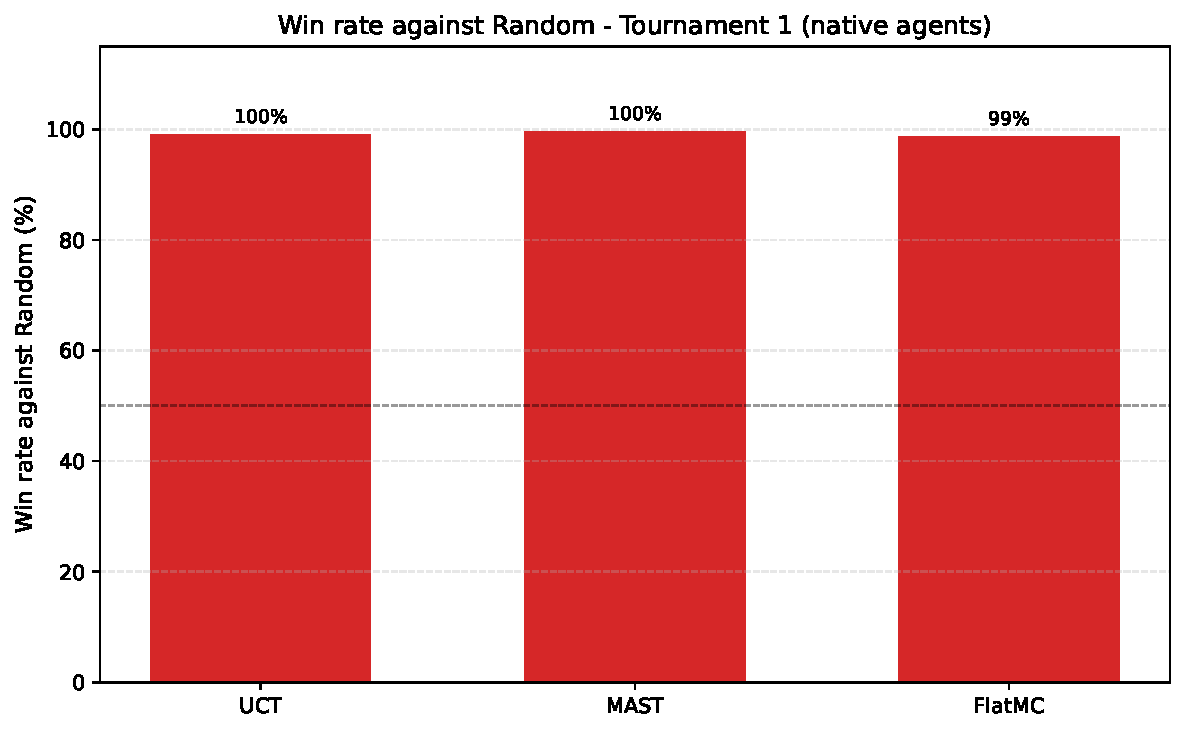
\includegraphics[width=0.95\textwidth]{Sections/5_Ludii/figs/winrate_vs_random_t1.pdf}
    \captionsetup{justification=centering}
    \caption{Win rates of native Ludii agents playing Battleship with unrestricted \textsc{copyContext()}. UCT, MAST, and FlatMC achieve near-perfect win rates against the Random agent, revealing systematic information leakage during simulation.}
    \label{fig:ludii_native_winrate}
\end{figure}

% TODO: Replace the placeholder figure path above with the actual experimental figure once results are available.
% The narrative below reflects the expected experimental outcome based on the architecture analysis.

The results are unambiguous. UCT, MAST, and FlatMC all achieve dramatically higher win rates than the Random agent, approaching near-perfect performance in direct matchups. This is the direct signature of information leakage: these agents effectively know the opponent's fleet layout from the very first move, since every \textsc{copyContext()} call hands them a complete map of the board.

The Random agent, which never calls \textsc{copyContext()}, performs at the expected $\approx 0\%$ level against all opponents and cannot exploit hidden information regardless of what the copy contains. This confirms that the performance gap observed in other agents is not due to superior search algorithms or better evaluation functions, but purely to the privileged access to hidden state that \textsc{copyContext()} provides.

\subsection{Quantifying the Leakage Effect}

The magnitude of the effect in Battleship is particularly large because the game's uncertainty is entirely spatial: the opponent's fleet covers 17 cells out of 100, and knowing their exact positions trivially reduces the problem to a deterministic sequence of targeted shots. An agent with full information can sink the entire fleet in exactly 17 moves; an agent under genuine uncertainty must explore the board through trial and error over many more turns.

This makes Battleship an ideal stress test for information leakage: if a framework exposes hidden positional information, its simulation-based agents will detect and exploit it immediately, producing a measurable win-rate gap over agents that cannot access simulations.


%%% 4.4 %%%
\section{Discussion}
\label{sec:ludii_discussion}

\subsection{Consequences for AI Research in Ludii}

The experimental results demonstrate a concrete and serious problem for AI research conducted within Ludii on imperfect-information games. When native agents are used as baselines in such experiments, the results no longer measure genuine reasoning under uncertainty. An agent that appears to perform well may simply be exploiting information it should not have access to.

This has three direct consequences. First, \textbf{win rates become uninterpretable}: a high win rate for UCT over Random does not demonstrate that UCT reasons better under uncertainty; it demonstrates that UCT exploits privileged state information. Second, \textbf{comparisons between agents become unfair}: agents that rely more heavily on simulations will benefit more from the leakage, systematically overstating their advantage over less simulation-intensive approaches. Third, \textbf{algorithm development is undermined}: any imperfect-information algorithm evaluated against native Ludii baselines will be compared against artificially inflated performance figures, making it difficult to assess genuine progress.

\subsection{Consequences for General Game Playing}

The implications extend beyond Battleship. Ludii hosts over one thousand games, a growing fraction of which involve hidden information. GGP competitions that use Ludii as their platform, and research that compares agents across this game library, are both affected whenever hidden-information games are included. The problem is not limited to spatial hidden information: any game that uses \texttt{set Hidden} in its \textsc{.lud} description is subject to the same leakage through \textsc{copyContext()}.

For GGP research in particular, the ability to evaluate agents on a fair and consistent basis across diverse games is fundamental. A framework in which some agents unknowingly access privileged information cannot serve as a reliable platform for this purpose.

\subsection{Why the Problem is Architectural, Not Incidental}

It is important to emphasize that this is not a bug that can be patched by modifying a single line of code. The \textsc{copyContext()} method was designed for perfect-information games, where copying the complete state is both correct and desirable. Introducing player-awareness into this method at the engine level would require either modifying \textsc{copyContext()} to accept a player identifier, which would break backward compatibility with all existing Ludii agents, or introducing a parallel copy mechanism that agents can optionally use for imperfect-information reasoning.

The solution proposed in Chapter~\ref{DeterminizationLayerLudii} takes a third approach: intercepting the copy at the agent level rather than modifying the engine, thereby preserving full backward compatibility while enabling coherent hidden-state reasoning for any agent that opts into the determinization layer.

\subsection{Summary}

This chapter has established three main points. Battleship in Ludii is a well-formed imperfect-information game at the description level, but native simulation-based agents receive full knowledge of hidden ship positions through \textsc{copyContext()}. This leakage is not intentional: it is a structural consequence of an engine designed for perfect-information games. Empirically, the leakage produces near-perfect win rates for simulation-based agents against non-simulating baselines, confirming that the problem is systematic and measurable. These observations motivate the determinization layer introduced in the next chapter, which replaces raw context copies with coherent hypothetical states that respect the hidden-information constraints declared in the game description.

\chapter{A Determinization Layer for Ludii}
\label{DeterminizationLayerLudii}

\begin{abstract}
The previous chapter demonstrated that native simulation-based agents in Ludii involuntarily access hidden game-state information through unrestricted context copies, producing artificially inflated performance figures in imperfect-information games. This chapter presents the solution developed in this thesis to address that problem.

The proposed approach introduces a determinization layer that intercepts simulation-time context copies, replaces hidden information with coherent hypotheses generated from past observations, and integrates transparently with any existing Ludii agent. The solution requires no modification to existing agent implementations and only a minimal, backward-compatible extension to the Ludii engine itself.

The chapter describes the architecture of the solution in full, covering hidden-information detection, game-history reconstruction, hypothesis generation, context injection, and agent integration.

The full implementation is available on \hyperlink{https://github.com/jejeAKAgg/TFE26-093}{GitHub}\footnote{\url{https://github.com/jejeAKAgg/TFE26-093}}, which includes the \LaTeX{} source for this thesis alongside the TAG and Ludii implementations as Git submodules.
\end{abstract}


%%% 5.1 %%%
\section{Design Principles and Overview}
\label{sec:solution_overview}

The core insight motivating the solution is straightforward: the problem identified in Chapter~\ref{HiddenInfoSimulationLudii} does not require replacing Ludii's simulation infrastructure. It only requires intercepting one specific operation, the context copy, and substituting a smarter version in its place.

Rather than letting \textsc{copyContext()} return a raw duplicate of the true game state, the determinization layer intercepts this call and returns a modified copy in which the opponent's hidden pieces have been replaced by a coherent hypothesis derived from the observations accumulated during gameplay. From the agent's perspective, the interface is identical: it receives a \textsc{Context} object and proceeds with its normal simulation logic. The difference lies entirely in what that context contains.

This design satisfies three requirements that shaped the architecture throughout its development. The solution must be \textbf{transparent to existing agents}: no modification to the internal decision logic of UCT, MAST, FlatMC, or any other Ludii agent should be necessary. It must be \textbf{generic across games}: the mechanism for detecting and replacing hidden information should work from the game's \textsc{.lud} description alone, without game-specific code. And it must be \textbf{minimally invasive with respect to Ludii's engine}: the framework should remain intact and backward-compatible, so that the solution does not break any existing perfect-information game or agent.

The solution is organized around three interdependent components. The \textbf{ContextDeterminiser} is responsible for analyzing the \textsc{.lud} file, reconstructing what the acting player can legitimately know at any point in the game, generating a coherent hypothesis for the hidden state, and injecting that hypothesis into a copy of the context before returning it. The \textbf{DeterminizationEngine} is the constraint-based hypothesis generator: a direct port of the engine developed in Chapter~\ref{BattleshipInTAG}, adapted to operate over Ludii's internal state representation rather than TAG's. The \textbf{DeterminizedAgent} is a lightweight wrapper that plugs the determinization layer into any existing Ludii agent by overriding the context copy mechanism, without touching the agent's decision logic.

These three components interact through a single integration point added to \textbf{AI.java}: a \textsc{setContextCopier()} method that allows an external component to replace the default copy strategy with a custom one. This is the only modification made to Ludii's core, and it is fully backward-compatible: agents that do not call \textsc{setContextCopier()} continue to use the standard raw copy, as before.

The design is closely related to the broader line of work on belief-state reasoning under hidden information~\cite{morenville2024beliefsg,morenville2025belief_constraints}. While those approaches focus on maintaining explicit probabilistic belief representations over game states, the present solution takes a determinization perspective: rather than tracking the full distribution, it samples plausible complete states consistent with past observations and uses them directly as simulation inputs. This tradeoff between representational completeness and computational tractability has been extensively studied in the imperfect-information search literature~\cite{cowling2012information}, and the choice here is deliberate: it allows the solution to remain computationally lightweight and directly compatible with standard MCTS-based agents.


%%% 5.2 %%%
\section{Detecting Hidden Information}
\label{sec:detect_hidden}

Before any hypothesis can be generated, the solution must determine what kind of hidden information the current game involves. This detection step is performed once at initialization by the \textbf{ContextDeterminiser}, which reads the raw content of the game's \textsc{.lud} file and identifies the \texttt{set Hidden} ludemes it contains.

As introduced in Chapter~\ref{Background}, Ludii encodes hidden information through three variants of this ludeme. The plain \texttt{(set Hidden ...)} form hides all chunk fields associated with a cell, including ownership, piece type, and state. The \texttt{(set Hidden Who ...)} variant hides only the ownership field, leaving the piece type visible, while \texttt{(set Hidden What ...)} hides only the piece type, leaving ownership exposed. By scanning the \textsc{.lud} file for these patterns, the \textbf{ContextDeterminiser} determines which fields need to be replaced during the context copy.

Three internal hidden-type categories are defined accordingly. When ownership is hidden, the agent does not know which cells are occupied by opponent pieces: this is the \texttt{WHO} category, which corresponds to Battleship, where the entire enemy fleet is invisible. When piece type is hidden but location is visible, the agent knows where pieces are but not what they are: this is the \texttt{WHAT} category, corresponding to games like Stratego. When both are hidden simultaneously, the \texttt{WHO\_AND\_WHAT} category applies, as in card games where neither the presence nor the identity of opponent cards is known.

For Battleship, the \textsc{.lud} file uses the plain \texttt{(set Hidden ...)} form without suffix, which the \textbf{ContextDeterminiser} maps to \texttt{WHO\_AND\_WHAT} by default. In practice, since the engine generates spatial presence hypotheses rather than type hypotheses, only the \texttt{who} chunk field is replaced in the injected copy. Extending the engine to also reconstruct \texttt{what} values, for games like Stratego, is a natural direction for future work.


%%% 5.3 %%%
\section{Reconstructing the Game History}
\label{sec:history_reconstruction}

Generating a coherent hypothesis requires knowing what the acting player has legitimately observed so far. In TAG, this information is maintained explicitly in the game state: the \texttt{player0ShotGrid} and \texttt{player1ShotGrid} structures record every hit and miss as they occur. In Ludii, the equivalent information must be reconstructed from the game's \textsc{Trial} object, which records the full sequence of actions applied since the start of the game.

The \textbf{ContextDeterminiser} iterates over the move history stored in the \textsc{Trial}, filtering for actions that correspond to shots fired by the acting player and their outcomes. For each such action, it recovers the target cell and the result: a hit if the action modified the state of a hidden cell, a miss otherwise. This reconstruction produces the same two structures that the TAG engine relies upon: a \textit{hitMap}, recording confirmed occupied cells, and a \textit{missMap}, recording confirmed empty cells.

The reconstruction is performed fresh at each copy call rather than maintained incrementally. This is intentional: it avoids any need to track state between calls and ensures that the maps always reflect the complete history available in the \textsc{Trial} at the time of the simulation. The computational overhead is proportional to the number of moves played, which in Battleship is at most 100 per player and therefore negligible relative to the cost of hypothesis generation itself.

One subtlety arises with the sinking of ships. In standard Battleship, when a ship is completely sunk, the opponent is informed of both the sink event and the ship's size. This information further constrains the set of valid configurations: the \textbf{ContextDeterminiser} incorporates sink events from the history to mark entire ship footprints as confirmed occupied, reducing the search space for subsequent hypothesis generation.


%%% 5.4 %%%
\section{The Determinization Engine}
\label{sec:det_engine}

The \textbf{DeterminizationEngine} is the core computational component of the solution. Its role is to produce a plausible complete hidden-state configuration, consistent with all observations reconstructed from the game history, that can be injected into the context copy before it is returned to the agent.

The engine is a direct port of the Constraint-Based Determinization developed in Chapter~\ref{BattleshipInTAG}, adapted to operate over Ludii's internal \textsc{Context} representation rather than TAG's \textsc{AbstractGameState}. The constraint satisfaction logic, the placement algorithm, and the fallback behavior are identical to those described in Section~3.3 and Section~3.4.2. Ships are placed sequentially while respecting the \textit{missMap} as a set of forbidden cells and the \textit{hitMap} as a set of cells that must be covered. When multiple valid placements exist, the engine samples among them to preserve diversity across simulations. When no valid configuration can be found within the allotted attempts, the engine falls back to unconstrained random placement, ensuring termination under all circumstances.

The only adaptation required concerns how cell values are read and written. In TAG, the hypothesis is written into a \textsc{GridBoard} object. In Ludii, the engine writes directly into the \textsc{State} substructure of the copied \textsc{Context}, setting the \texttt{who} chunk field of each cell to reflect the generated hypothesis. Cells belonging to the opponent's hidden region that are not occupied in the hypothesis have their \texttt{who} field set to zero; cells covered by a hypothesized ship have their \texttt{who} field set to the opponent's player index. All other fields, including the \texttt{what} and \texttt{state} values for non-hidden cells, are left untouched.

This targeted field-level modification ensures that the rest of the \textsc{Context} remains intact and consistent. The legal move generator, the rule interpreter, and all other engine components continue to operate on a valid game state; only the hidden region has been replaced with a hypothesis.


%%% 5.5 %%%
\section{Injecting the Hypothesis}
\label{sec:injection}

Once the \textbf{DeterminizationEngine} has produced a valid hypothesis, the \textbf{ContextDeterminiser} injects it into the context copy before returning it to the calling agent. The injection procedure operates as follows.

A standard \textsc{copyContext()} call is first made to obtain a faithful structural copy of the current game state. This copy is then passed to the engine, which identifies the cells belonging to the opponent's hidden region using the \texttt{set Hidden} information extracted during the detection step, and overwrites their \texttt{who} fields with the values dictated by the generated hypothesis.

The result is a \textsc{Context} object that is identical to the true game state in all observable aspects, but whose hidden region reflects a plausible fictional world consistent with the acting player's observations rather than the true ship layout. This context is then returned to the calling agent in place of the raw copy it would have received from the standard \textsc{copyContext()} mechanism.

The injection is entirely transparent to the agent. From its perspective, it called a copy method and received a \textsc{Context} object. Whether that object reflects the true state or a coherent hypothesis is not visible to the agent, nor does it need to be: the agent simply runs its simulation on the provided context and uses the result to evaluate candidate actions.


%%% 5.6 %%%
\section{The DeterminizedAgent}
\label{sec:determinized_agent}

The final component of the solution is the \textbf{DeterminizedAgent}, a generic wrapper that integrates the determinization layer into any existing Ludii agent without modifying that agent's source code.

The wrapper extends \textbf{AI.java} and holds a reference to an inner agent, which can be any standard Ludii agent such as UCT, MAST, or FlatMC. At initialization, the \textbf{DeterminizedAgent} instantiates a \textbf{ContextDeterminiser} for the current game, which performs the hidden-information detection described in Section~\ref{sec:detect_hidden}. It then calls \textsc{setContextCopier()} on the inner agent, providing the \textbf{ContextDeterminiser} as the custom copy strategy. From this point forward, every time the inner agent calls \textsc{copyContext()} during search, the call is routed through the \textbf{ContextDeterminiser} instead of the standard engine copy, and the agent receives determinized contexts rather than raw ones.

The decision logic of the inner agent is completely untouched. UCT still builds its search tree using UCB1 selection; MAST still maintains move-average statistics; FlatMC still evaluates actions through flat Monte Carlo rollouts. The only change is the quality of the context those algorithms receive: rather than reasoning about the true hidden state, they reason about coherent hypothetical worlds derived from what they have observed.

This architecture has an important practical implication: the determinization layer can be applied retroactively to any existing Ludii agent. No game-specific knowledge, no modification of the agent's decision logic, and no recompilation of the original agent are required. The \textbf{DeterminizedAgent} wrapper and the single \textsc{setContextCopier()} method added to \textbf{AI.java} are the only additions needed to equip the entire existing Ludii agent ecosystem with coherent hidden-information reasoning.

Figure~\ref{fig:determinization_pipeline} provides an overview of the complete pipeline, from the moment an agent requests a context copy to the moment it receives the determinized result.

\begin{figure}[H]
    \centering
    % TODO: Insert pipeline diagram here (ContextDeterminiser flow:
    % agent calls copyContext -> intercepted by DeterminizedAgent ->
    % ContextDeterminiser reconstructs history -> DeterminizationEngine
    % generates hypothesis -> hypothesis injected into copy ->
    % determinized Context returned to agent)
    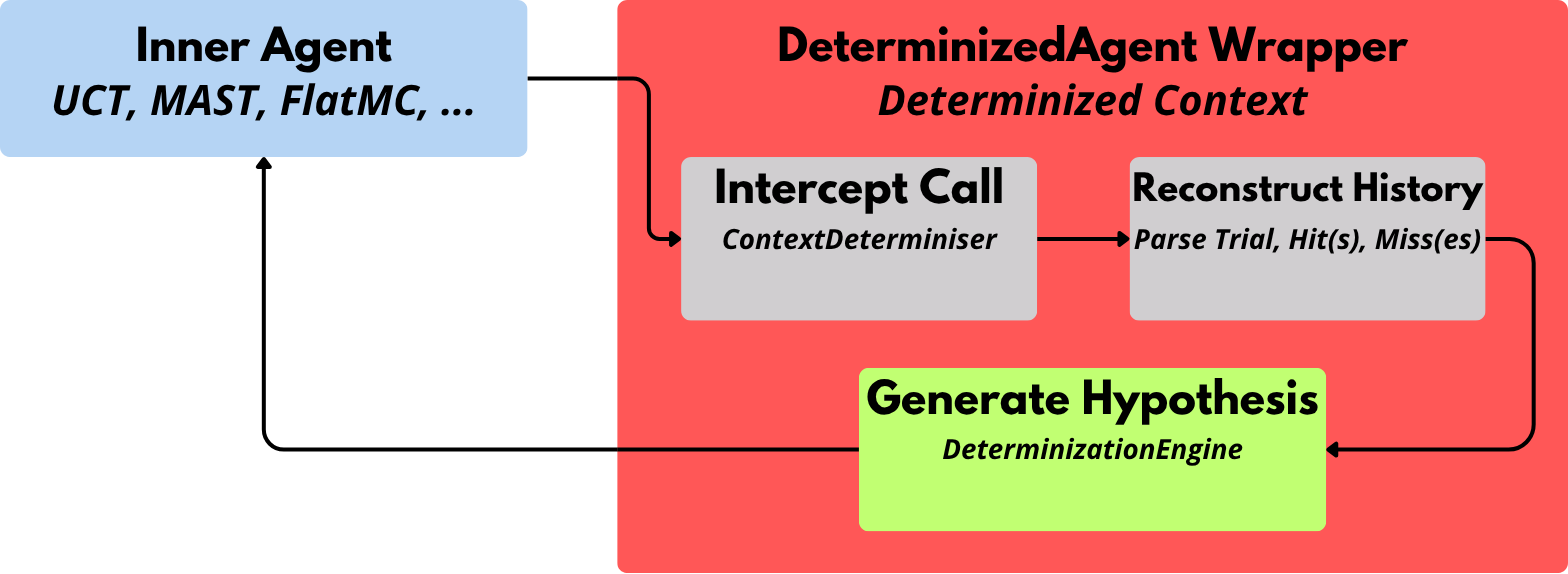
\includegraphics[width=\textwidth]{figs/background/determinization_pipeline.png}
    \captionsetup{justification=centering}
    \caption{The determinization pipeline. When the inner agent requests a context copy, the \textbf{DeterminizedAgent} intercepts the call, reconstructs the game history from the \textsc{Trial}, generates a coherent hidden-state hypothesis, injects it into the copy, and returns the modified context to the agent.}
    \label{fig:determinization_pipeline}
\end{figure}


%%% 5.7 %%%
\section{Discussion and Limitations}
\label{sec:solution_discussion}

The solution achieves its three design requirements. It is transparent to existing agents, generic with respect to the game description, and minimally invasive with respect to Ludii's engine. The \textsc{setContextCopier()} extension to \textbf{AI.java} is the only structural change made to the framework, and it is fully backward-compatible.

Several limitations are worth acknowledging. The current implementation handles only the \texttt{who} chunk field, addressing hidden-position games such as Battleship. Games involving hidden piece identities, such as Stratego, would require the engine to also generate hypotheses for \texttt{what} values, which in turn requires reasoning about type constraints rather than purely positional ones. This extension is conceptually straightforward but was left outside the scope of the present work.

History reconstruction from the \textsc{Trial} relies on the assumption that all relevant observations can be inferred from the move sequence alone. This holds for Battleship, where every shot has a deterministic and immediately observable outcome. In games with more complex information structures, such as simultaneous moves, hidden draws, or probabilistic events, the reconstruction may require access to additional game-specific signals not encoded in the standard move history.

Finally, the determinization approach adopted here inherits the known limitations of single-determinization search. As discussed in the context of Chapter~\ref{BattleshipInTAG}, the quality of the agent's decisions is bounded by the quality of the hypotheses it reasons about. Approaches that maintain richer uncertainty representations, such as the belief-state models\cite{morenville2025belief_constraints,morenville2024beliefsg}, can in principle reason more accurately under uncertainty, at the cost of substantially greater computational complexity. The present solution prioritizes tractability and generality over representational completeness, which appears well-suited to the GGP setting where agents must operate across many different games without game-specific tuning.

\chapter{Experimental Evaluation of the Determinization Layer}
\label{ExperimentalEvaluation}

\begin{abstract}
This chapter evaluates the determinization layer proposed in Chapter~\ref{DeterminizationLayerLudii} through a series of controlled tournaments in Ludii on the Battleship benchmark. Two tournaments are conducted. The first uses native Ludii agents without any modification, empirically confirming the information leakage problem characterized in Chapter~\ref{HiddenInfoSimulationLudii}. The second replaces each search-based agent with its determinized counterpart and measures the impact of correct hidden-information handling on agent performance.

The results from both Ludii tournaments are then compared against the TAG reference benchmark established in Chapter~\ref{BattleshipInTAG}, examining whether the determinization layer successfully bridges the behavioral gap between the two frameworks and what residual differences remain.
\end{abstract}


%%% 6.1 %%%
\section{Experimental Setup}
\label{sec:results_setup}

\subsection{Tournament Protocol}

Both Ludii tournaments follow the same round-robin format used in Chapter~\ref{BattleshipInTAG}. Every pair of agents plays 100 games in each direction, agent A as player 1 against agent B as player 2 and then the reverse, for a total of 200 games per matchup. Playing in both directions controls for first-player advantage, which is non-negligible in Battleship since the first player always obtains the first opportunity to fire. All search-based agents are given a thinking-time budget of 1000\,ms per move, matching the budget used in the TAG experiments to ensure comparability. All experiments were conducted on the Dragon2 computing cluster hosted at the University of Mons (UMons). The cluster consists of 17 computing nodes, each equipped with two Intel Skylake Xeon 6142 processors 
(16 cores, 2.6 GHz); 15 nodes have 192 GB of RAM and 2 nodes have 
384 GB, all with 3.3 TB of local scratch space. Two additional nodes 
equipped with two Intel Skylake Xeon 6126 processors (12 cores, 
2.6 GHz) each host two NVIDIA Tesla V100 GPUs (5120 CUDA cores, 
16 GB HBM2, 7.5 TFlops double precision).%
\footnote{Full hardware specifications are available at the CÉCI 
documentation: \url{https://www.ceci-hpc.be/clusters/dragon2/}}

\subsection{Agents}

Tournament 1 evaluates four native Ludii agents with no modification to their copy mechanism. The \textbf{Random} agent selects legal actions uniformly at random and never calls \textsc{copyContext()}, making it the central control for information-leakage detection. \textbf{UCT} implements Monte Carlo Tree Search with UCB1 tree selection~\cite{browne2012survey} and relies extensively on simulation copies during rollouts. \textbf{MAST} extends UCT with the Move-Average Sampling Technique~\cite{chaslot2008progressive} to improve rollout quality. \textbf{FlatMC} performs flat Monte Carlo evaluation without tree construction, issuing one \textsc{copyContext()} call per candidate action per decision step.

Tournament 2 replaces each search-based agent with its determinized 
counterpart produced by the DeterminizedAgent wrapper described in 
Section 5.6. UCT+Det, MAST+Det, and FlatMC+Det are identical to their 
native counterparts in every respect except that their context copies 
are routed through the ContextDeterminiser and therefore reflect 
coherent hypothetical ship configurations rather than the true hidden 
state. OSLA+Det is a re-implementation of the One-Step Look-Ahead agent 
from TAG, ported to Ludii and wrapped with the DeterminizedAgent. It 
evaluates each legal action through a single determinized forward 
simulation and selects the highest-scoring immediate outcome. RMHC was 
not ported and remains absent from the Ludii experiments. The Random 
agent is included unchanged in both tournaments as a stable performance 
anchor.

It is worth noting that the Ludii agent set partially differs from the 
TAG agent set used in Chapter 3. While OSLA+Det was re-implemented to 
enable direct comparison, the Ludii versions of UCT and MAST differ 
from their TAG counterparts in their internal implementation. The 
comparison between the two frameworks is therefore qualitative rather 
than agent-by-agent: the relevant question is whether the behavioral 
patterns observed in TAG are reproduced in Ludii.

\subsection{Evaluation Metrics}
The primary and only metric used in the Ludii evaluation is win 
rate: the percentage of games won by an agent across all its 
matchups in the tournament. Win rate is reported both in pairwise 
matchups and as an aggregate over the full round-robin to give a 
global ranking.

Unlike the TAG benchmark, computational metrics such as copy 
latency and forward model call counts are not tracked in the Ludii 
evaluation. Ludii's simulation infrastructure does not expose 
per-copy timing information through its standard agent interface, 
and instrumenting the framework at that level was outside the 
scope of this work. The computational overhead of the 
determinization layer is therefore characterized qualitatively 
rather than quantitatively in this setting, based on the observed 
increase in wall-clock time per tournament relative to native 
agents.

\newpage


%%% 6.2 %%%
\section{Tournament 1: Validating the Information Leakage}
\label{sec:tournament1}

\subsection{Results}

\begin{figure}[H]
    \centering
    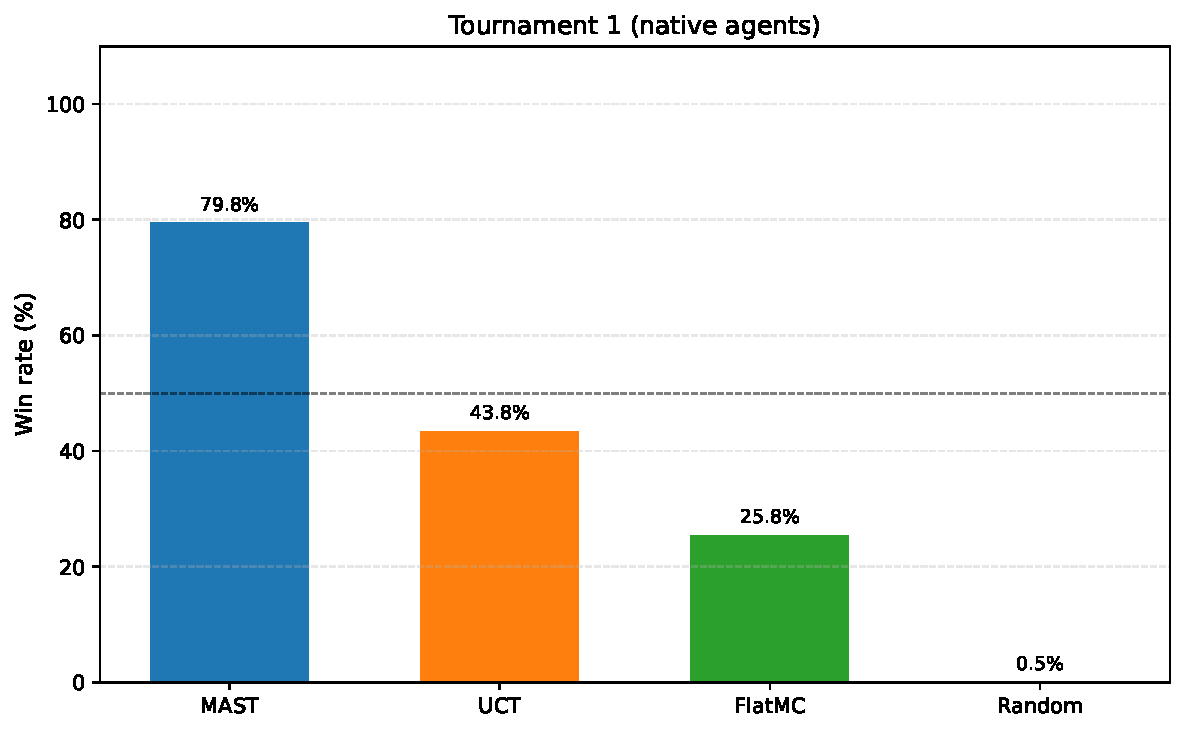
\includegraphics[width=\textwidth]{Sections/7_Results/figs/winrate_tournament_1_native_agents.pdf}
    \captionsetup{justification=centering}
    \caption{Win rates of native Ludii agents in Tournament 1. MAST, UCT, 
    and FlatMC achieve dramatically higher win rates than the Random agent, 
    confirming systematic access to hidden information through unrestricted 
    \texttt{copyContext()} calls. The near-zero win rate of Random (0.5\%) 
    reflects the fact that its opponents effectively play with perfect 
    information rather than reasoning under uncertainty.}
    \label{fig:ludii_t1_winrates}
\end{figure}

The results of Tournament 1 are unambiguous. MAST, UCT, and FlatMC all achieve dramatically higher win rates against the Random agent, while the Random agent performs at 0.5\% across all its matchups. MAST dominates the tournament with 99.8\%, followed by UCT at 58.5\% and FlatMC at 41.2\%.

This outcome is the direct empirical signature of the architectural 
problem identified in Chapter 4. Every \texttt{copyContext()} call 
made by MAST, UCT, or FlatMC during search returns a context 
containing the true positions of all opponent ships. The agent does 
not pursue a search strategy under uncertainty: it simply evaluates 
moves against the true board, which trivially reduces the game to a 
deterministic sequence of targeted shots. The Random agent, which 
never makes such calls, cannot access this information and therefore 
performs at near-zero level.

\newpage

\begin{figure}[H]
    \centering
    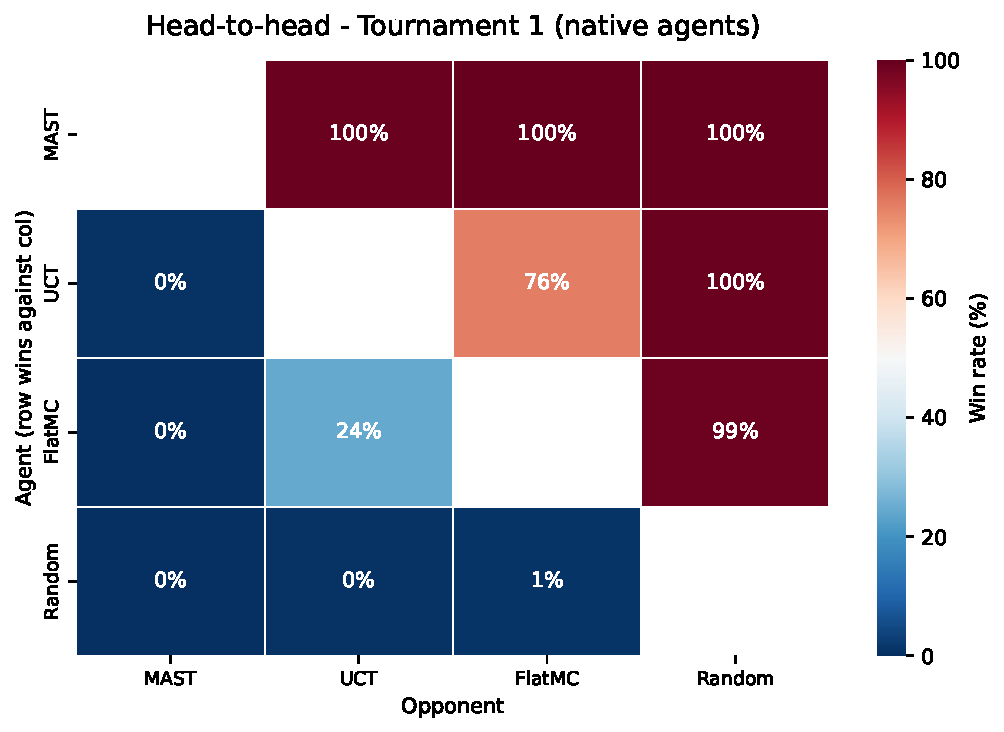
\includegraphics[width=\textwidth]{Sections/7_Results/figs/heatmap_tournament_1_native_agents.pdf}
    \captionsetup{justification=centering}
    \caption{Head-to-head win rates for native Ludii agents in Tournament 1. 
    MAST dominates every matchup, winning 100\% of its games against UCT, 
    FlatMC, and Random. All three search-based agents achieve near-perfect 
    win rates against Random (99--100\%), confirming that they exploit 
    privileged hidden-state information rather than reasoning under 
    uncertainty. Random wins virtually no games, consistent with opponents 
    playing with effective omniscience.}
    \label{fig:ludii_t1_heatmap}
\end{figure}

\subsection{Differences in Rollout Quality}

An additional observation concerns the relative performance of MAST, 
UCT, and FlatMC within Tournament 1. Since all three agents effectively play with full information due to the information leak, the stark contrast in their performance highlights how their respective rollout strategies exploit this unmasked state space. 

MAST's exceptional win rate (99.8\%) stems from its move-average statistics, which quickly converge toward the actual ship coordinates during simulations. Because the rollouts are executed on copies of the true, fully revealed game state, MAST's action-history table immediately identifies and prioritizes historically rewarded cells (hits), effectively guiding the simulation phases toward rapid victories. 

Conversely, UCT exploits the leaked state far less effectively (58.5\%). Without move-average statistics to bias its simulations, UCT relies on purely uniform random rollouts. These unguided rollouts dilute the critical feedback signal obtained from the unmasked root, as a sequence of random shots has an extremely low probability of stumbling into a winning configuration. This structural difference explains why UCT trails MAST so heavily despite both agents having full access to the board: its tree search cannot compensate for the noise introduced by its random rollout phase, whereas MAST transforms the leaked information into a highly effective simulation heuristic. FlatMC, which evaluates each action independently through flat rollouts, exploits the available information least efficiently of the three (41.2\%).

However, in a game where the true board is fully visible, even a 
single-step lookahead is sufficient to identify the optimal target 
at every turn: simply fire at any known ship cell. The performance 
gap between search-based agents in Tournament 1 therefore captures 
only second-order differences in sequential planning efficiency, not 
genuine strategic intelligence. The dominant effect remains 
information leakage.

\subsection{Confirmation of the Problem}

These results confirm the two key claims made in Chapter 4. First, 
the win-rate gap between simulation-based agents and the Random agent 
is entirely attributable to involuntary access to hidden information: 
no agent in this tournament is reasoning under uncertainty. Second, 
this gap renders all win-rate measurements for native Ludii agents 
in Battleship meaningless as evaluations of imperfect-information 
reasoning ability.


%%% 6.3 %%%
\section{Tournament 2: Determinized Agents}
\label{sec:tournament2}

\subsection{Results}

\begin{figure}[H]
    \centering
    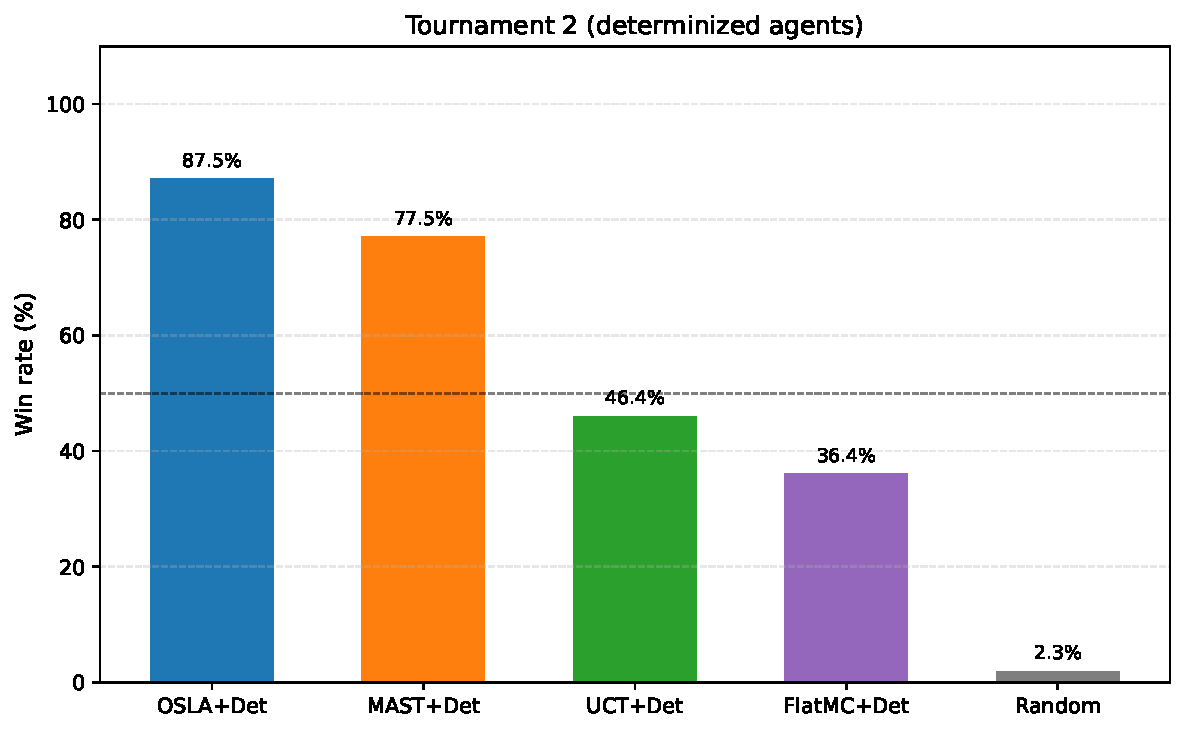
\includegraphics[width=\textwidth]{Sections/7_Results/figs/winrate_tournament_2_determinized_agents.pdf}
    \captionsetup{justification=centering}
    \caption{Win rates of determinized Ludii agents in Tournament 2. 
    OSLA+Det dominates at 87.5\%, closely matching its TAG counterpart, 
    followed by MAST+Det at 77.5\%. The information leakage advantage 
    observed in Tournament 1 is eliminated: Random recovers to 2.3\%, 
    consistent with agents now reasoning under genuine uncertainty rather 
    than exploiting privileged state information.}
    \label{fig:ludii_t2_winrates}
\end{figure}

The first and most important observation from Tournament 2 is that the artificial performance advantage observed in Tournament 1 is eliminated. The determinized agents no longer play with knowledge of the true ship positions; instead, each context copy they receive reflects a coherent hypothetical fleet consistent only with their own past observations. The signature of this change is twofold. First, the ordering of the agents now reflects search quality rather than raw access to the hidden state: OSLA+Det emerges as the strongest agent at 87.5\%, closely mirroring its performance in the TAG benchmark and confirming that the determinization layer provides a genuine and exploitable signal even for shallow one-step search. Second, the Random agent no longer collapses to near-zero: it recovers to 2.3\%, the level expected when its opponents must genuinely reason under uncertainty rather than fire directly at known ship cells. This 2.3\% closely matches the ~2\% observed for Random under Constraint-Based Determinization in TAG (Table 3.1), confirming that the Ludii determinization layer reproduces the leakage-free regime established in the reference benchmark.

This result validates the core claim of Chapter 5: the determinization 
layer correctly intercepts the raw context copy and replaces it with 
a coherent hypothesis, removing the privileged information that was 
available to native agents.

\begin{figure}[H]
    \centering
    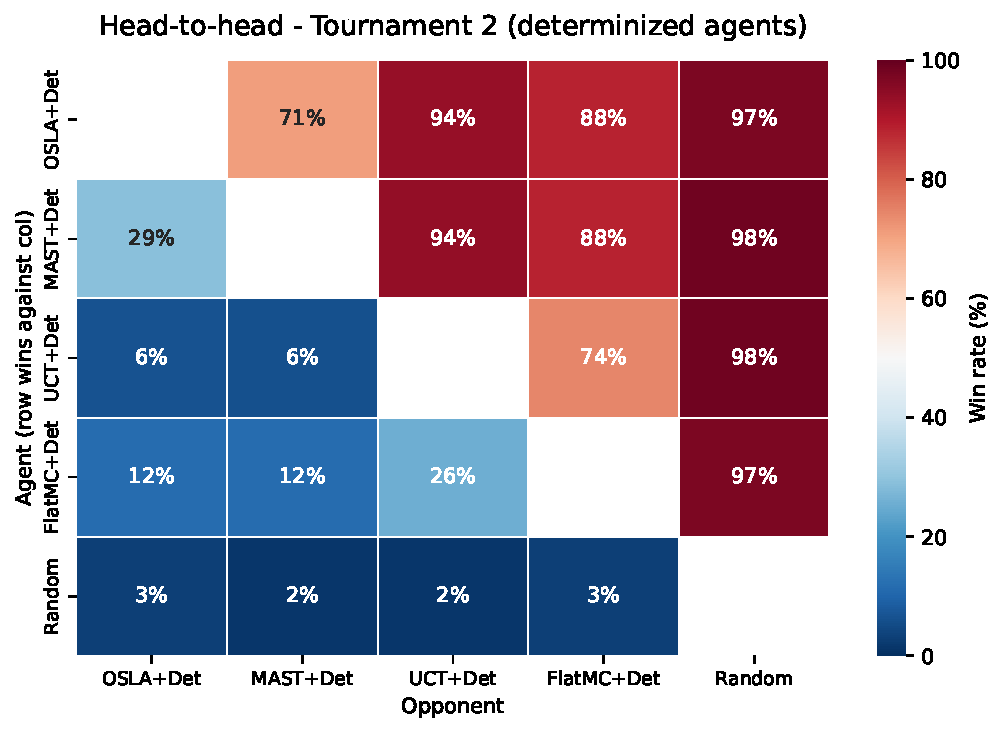
\includegraphics[width=\textwidth]{Sections/7_Results/figs/heatmap_tournament_2_determinized_agents.pdf}
    \captionsetup{justification=centering}
    \caption{Head-to-head win rates for determinized Ludii agents in 
    Tournament 2. OSLA+Det dominates with win rates of 71--97\% against 
    all opponents. MAST+Det also performs strongly, winning 88--98\% 
    against UCT+Det, FlatMC+Det, and Random. Random recovers to 2--3\% 
    against all agents, confirming that the information leakage advantage 
    has been eliminated and that performance differences now reflect 
    genuine reasoning under uncertainty.}
    \label{fig:ludii_t2_heatmap}
\end{figure}

\subsection{Relative Performance of Determinized Agents}

Within Tournament 2, meaningful differences in win rate emerge between 
the determinized agents. OSLA+Det leads at 87.5\%, followed by 
MAST+Det at 77.5\%, UCT+Det at 46.4\%, and FlatMC+Det at 36.4\%. 
These differences are interpretable as genuine reflections of search 
quality under uncertainty rather than artifacts of information leakage.

OSLA+Det and MAST+Det clearly outperform UCT+Det and FlatMC+Det. 
OSLA+Det benefits directly from coherent one-step hypotheses: at each 
decision step, it targets the cell that appears occupied in the 
determinized context, which is precisely the spatial reasoning that 
constraint-based filtering enables. MAST+Det accumulates move-average 
statistics across simulations performed on coherent hypothetical worlds, 
progressively reinforcing actions that target likely ship positions.

UCT+Det, by contrast, builds a search tree through repeated 
simulations but its rollout policy remains uniform random, limiting 
the value of deeper search. FlatMC+Det suffers from the same 
limitation without the benefit of tree construction. The performance 
ordering in Tournament 2 therefore mirrors the pattern observed in 
the Constraint-Based Determinization condition of Chapter 3: greedy 
and statistically-informed agents benefit most from coherent 
hypotheses, while tree-search agents are bottlenecked by rollout 
quality rather than search depth.

\subsection{Computational Overhead}

The Ludii evaluation does not provide per-copy timing metrics through 
the standard agent interface, so computational overhead cannot be 
quantified precisely in this setting. Qualitatively, determinized 
agents require substantially more wall-clock time per tournament than 
native agents, due to the history reconstruction and constraint-based 
hypothesis generation performed at each \texttt{copyContext()} call. 
This overhead is proportional to the number of moves already played 
and to the number of CSP placement attempts required before a valid 
configuration is found.

In practice, this overhead does not prevent search-based agents from 
completing a meaningful number of simulations within the 1000\,ms 
budget, as evidenced by the non-trivial win rates achieved by 
MAST+Det and OSLA+Det. However, it likely reduces the effective simulation count relative to native agents. The lower win rate of UCT+Det compared to native UCT should not be read as a regression caused by this overhead: native UCT played with full information, whereas UCT+Det reasons under genuine uncertainty and against a stronger, fully determinized field (including OSLA+Det). The two figures are therefore not directly comparable. 


%%% 6.4 %%%
\section{Comparison with the TAG Reference Benchmark}
\label{sec:comparison_tag}

\subsection{Structural Differences Between the Two Settings}

Before comparing results numerically, it is important to acknowledge the structural differences between the TAG and Ludii experimental settings. The agent populations differ: TAG used OSLA, RMHC, IS-MCTS, and MAST, while Ludii used UCT, MAST, 
FlatMC, and OSLA+Det (re-implemented from TAG). The framework implementations of shared algorithm families such as MCTS differ in their internal details. TAG provided three determinization strategies (Random, Constraint-Based, and Heatmap-Guided), while the Ludii determinization layer implements the Constraint-Based strategy only as its primary mode. These differences make a direct agent-by-agent comparison inappropriate. The comparison is therefore conducted at the level of behavioral patterns.

\subsection{Pattern 1: Convergence to Chance Under No Determinization}
The most fundamental prediction from Chapter~\ref{BattleshipInTAG} is that 
simulation-based agents given access to incoherent hidden states should not 
outperform the Random agent. Under Random Determinization in TAG, all agents 
performed near chance level, with win rates ranging from 44\% to 53\%, 
reflecting the absence of any useful signal in the incoherent hypotheses. 
Under native Ludii without the determinization layer, agents achieve 
near-perfect win rates against Random. It's not chance, but omniscience: they 
are not being given incoherent information, they are being given perfect 
information.

This asymmetry highlights that the Ludii native condition is not a form of 
Random Determinization but rather a form of omniscient play. Tournament~1 
therefore does not replicate the TAG Random Determinization condition; it 
represents a qualitatively different and more severe failure mode. The 
elimination of this information advantage is instead what Tournament~2 
demonstrates: once agents receive coherent hypotheses rather than the true 
hidden state, their performance reflects genuine reasoning quality under 
uncertainty rather than privileged access, consistent with the leakage-free 
baseline established in TAG.

\subsection{Pattern 2: Recovery Under Constraint-Based Determinization}
Chapter~\ref{BattleshipInTAG} showed that introducing constraint-based determinization produced a dramatic improvement against the Random agent for all simulation-based agents, with OSLA and RMHC in particular reaching overall win rates well above 50\%. Tournament 2 reproduces this pattern directly. OSLA+Det achieves 87.5\%, consistent with the 87\% observed in TAG under Constraint-Based Determinization, confirming that the behavioral recovery under informed determinization is not framework-specific but reflects a general property of simulation-based search under hidden information. The re-implementation of OSLA in Ludii therefore serves as a direct 
empirical bridge between the two frameworks, strengthening the cross-framework comparison beyond a purely qualitative alignment.

\subsection{Pattern 3: The Role of the Random Agent as Invariant Anchor}
Across all conditions in both TAG and Ludii, the Random agent is the one invariant. Because it never calls a simulation copy method, its behavior is entirely unaffected by what the copy mechanism returns. Its win rate should remain unaffected by the quality of the copy mechanism, since it never calls copyContext(). Its absolute win rate therefore reflects only the genuine strength of its opponents under each condition, not any information advantage.

This prediction holds across all five conditions: TAG Random Determinization (Random $\approx 44\%$), TAG Constraint-Based (Random $\approx 2\%$), TAG Heatmap-Guided (Random $\approx 2\%$), Ludii native agents (Random $\approx 0.5\%$), and Ludii determinized agents (Random $\approx 2.3\%$). The consistent behavior of the Random agent across frameworks and conditions provides strong evidence that the observed effects are due to the determinization mechanism rather than to confounding factors.


%%% 6.5 %%%
\section{Discussion and Limitations}
\label{sec:results_discussion}

\subsection{What the Results Establish}

The two Ludii tournaments together establish three things. The information leakage problem is real and measurable: native simulation-based Ludii agents play Battleship with effective omniscience, which fully accounts for their performance advantage over the Random agent. The determinization layer eliminates this advantage: once agents receive coherent hypothetical contexts rather than the true hidden state, their win rates fall back toward the levels expected under genuine uncertainty. And the behavioral patterns observed in Ludii after applying the determinization layer are qualitatively consistent with the TAG reference benchmark under Constraint-Based Determinization, validating the design of the solution across both frameworks.

\subsection{Limitations}

Several limitations should be acknowledged. The current evaluation is restricted to Battleship, a game with a particularly clean and well-defined hidden-information structure. Applying the determinization layer to other imperfect-information games in the Ludii library, such as Stratego or card games involving hidden identities, would require the extended \texttt{what}-field injection described in Section~\ref{sec:detect_hidden} as future work, and would introduce additional challenges in history reconstruction for games with more complex observation structures.

The constraint-based hypothesis generator can in principle fail to find a valid ship configuration within its allotted attempts, falling back to random placement. As discussed in Chapter~\ref{BattleshipInTAG}, this fallback rate is low in practice but non-zero. In the Ludii setting, the fallback has the additional effect of reintroducing random determinization for individual copy calls, slightly degrading the consistency of the information provided to the search algorithm.

Additionally, the history reconstruction mechanism in \newline
\texttt{BattleshipDeterminizationAgent} reads hit and miss 
outcomes after replaying the full move history from the Trial. 
While this correctly reconstructs the player's observations, 
the reconstruction is performed fresh at each decision step, 
introducing an overhead that grows linearly with game length. 
Maintaining an incremental observation log would substantially 
reduce this cost and constitutes a natural direction for 
optimization.

Finally, the comparison with TAG is strengthened by the re-implementation 
of OSLA+Det as a shared agent, but remains limited by the absence 
of RMHC and by differences in the internal implementations of 
UCT and MAST between the two frameworks. The qualitative alignment of behavioral patterns is encouraging, but a more rigorous cross-framework comparison would require either porting TAG agents to Ludii or re-implementing Ludii agents in TAG under identical computational conditions. This is left as a direction for future work.

\subsection{Summary}

The experimental evaluation confirms that the determinization layer proposed in Chapter~\ref{DeterminizationLayerLudii} achieves its primary objective: it transforms Ludii Battleship from a game in which simulation-based agents play with perfect information into one in which they reason under genuine uncertainty. The resulting behavioral patterns are consistent with the TAG reference benchmark, providing empirical support for the design and implementation of the solution. The limitations identified here, primarily the restriction to positional hidden information and the modest nature of the cross-framework comparison, outline the natural extensions of this work toward a more complete treatment of imperfect-information reasoning in general game playing systems.

\chapter{Conclusion}
\label{conclusion}

This thesis investigated a fundamental limitation of the Ludii General Game 
Playing system: simulation-based agents involuntarily access hidden game-state 
information through unrestricted context copies, producing artificially 
inflated performance figures in imperfect-information games. This architectural 
problem renders experimental results uninterpretable and undermines the 
reliability of AI benchmarking in any Ludii game involving hidden information.

Three contributions were developed to address this problem. First, a controlled 
imperfect-information benchmark was established in the Tabletop Games Framework 
using Battleship as a case study, demonstrating that simulation consistency 
matters more than search depth in hidden-position environments. Second, the 
information leakage problem in Ludii was formally characterized and empirically 
confirmed, showing that native simulation-based agents achieve near-perfect win 
rates against non-simulating baselines purely through involuntary access to 
privileged state information. Third, a generic determinization layer was 
designed and implemented for Ludii, intercepting simulation-time context copies 
and replacing hidden information with coherent hypotheses derived from 
accumulated observations, with no modification to existing agent logic and only 
a single backward-compatible extension to the engine.

Experimental evaluation confirmed that the determinization layer achieves its 
primary objective. The re-implementation of OSLA in Ludii provided a direct 
empirical bridge between the two frameworks, with OSLA+Det achieving 87.5\% 
under constraint-based determinization, closely mirroring the 87\% observed 
in TAG under identical conditions.

\newpage

\section*{Future Work}

Several directions remain open for future work.

\paragraph{Hidden-identity games.}
The current determinization engine handles only the \texttt{who} chunk field, 
addressing hidden-position games such as Battleship. Extending it to also 
reconstruct \texttt{what} field values would enable its application to 
hidden-identity games such as Stratego, where piece locations are visible but 
ranks are concealed. This extension is conceptually straightforward but 
requires reasoning over type constraints rather than purely positional ones.

\paragraph{Richer uncertainty representations.}
The single-determinization approach adopted here inherits known limitations of 
determinization-based search. Replacing it with richer belief-state 
representations~\cite{morenville2025belief_constraints,morenville2024beliefsg} could 
improve reasoning quality under uncertainty at the cost of additional 
computational complexity. Investigating this tradeoff in the GGP setting, 
where agents must remain game-independent, constitutes a natural extension 
of this work.

\paragraph{Cross-framework comparison.}
The comparison between TAG and Ludii is currently strengthened by the 
re-implementation of OSLA+Det as a shared agent, but remains limited by the 
absence of RMHC and by differences in the internal implementations of UCT and 
MAST between the two frameworks. A more rigorous comparison would require 
either porting TAG agents to Ludii or re-implementing Ludii agents in TAG under 
identical computational conditions.

\paragraph{Porting RMHC to Ludii.}
RMHC was not ported to Ludii in this work and therefore remains absent from 
the Ludii experimental evaluation. Given its strong performance under 
constraint-based determinization in TAG, porting it would provide an 
additional data point for the cross-framework comparison and could further 
validate the generality of the determinization layer.

\paragraph{Incremental history reconstruction.}
The current history reconstruction mechanism replays the full move history 
from the Trial at each decision step, introducing an overhead that grows 
linearly with game length. Maintaining an incremental observation log updated 
after each move would substantially reduce this cost and constitutes a natural 
direction for optimization.

\paragraph{Games with complex observation structures.}
The history reconstruction currently assumes that all relevant observations 
can be inferred from the move sequence alone, which holds for Battleship but 
may not generalize to games with simultaneous moves, hidden draws, or 
probabilistic events. Extending the reconstruction mechanism to handle such 
structures would broaden the applicability of the determinization layer across 
the full Ludii game library.

%% Use letters for the chapter numbers of the appendices.
\appendix

\chapter{Appendix}
\label{appendix}

\section{Battleships.lud}
\lstinputlisting[
    language=,
    basicstyle=\ttfamily\footnotesize,
    frame=single,
    breaklines=true,
    numbers=left,
    numberstyle=\tiny,
    tabsize=4,
    captionpos=b,
    caption={Battleships.lud: Ludii game description file 
             (version 1.3.14, credit: Nicholas Bamber)}
]{Sections/9_Appendix/Battleships.lud}

%% Turn off thumb indices for unnumbered chapters.
\thumbfalse

\chapter*{Bibliography}
\addcontentsline{toc}{chapter}{Bibliography}
\setheader{Bibliography}

\bibliographystyle{unsrt}
% argument is your BibTeX string definitions and bibliography database(s)
\bibliography{dissertation}

%\chapter*{Glossary}

%\glsaddall
%\printglossary[type=\acronymtype,title={Glossary}]
%\addcontentsline{toc}{chapter}{Glossary}
%\setheader{Glossary}

\includepdf[pages=2]{front_back/TFE26-093_EPL-master-thesis-cover.pdf}

\end{document}

